% !TEX program = xelatex
% 编译：在 paper/ 目录下运行 latexmk -xelatex main.tex（会自动调用 biber）
\documentclass[a4paper,zihao=-4,openany]{ctexrep}
% 公共导言区：所有章节共用。新增宏请写在这里，不要写进章节文件。
\usepackage[a4paper,top=2.6cm,bottom=2.6cm,left=2.6cm,right=2.6cm]{geometry}
\usepackage{amsmath,amssymb,mathtools,bm}
\usepackage{graphicx}
\usepackage{booktabs,tabularx,longtable,multirow,array}
\usepackage[table]{xcolor}
\usepackage{caption,subcaption}
\usepackage{float}
\usepackage{enumitem}
\usepackage{siunitx}
\usepackage[most]{tcolorbox}
\usepackage[backend=biber,style=gb7714-2015,gbpub=false,gbnamefmt=lowercase]{biblatex}
\usepackage[hidelinks]{hyperref}
\usepackage[capitalise,noabbrev]{cleveref}

\graphicspath{{../figures/}}
\setlist{nosep,leftmargin=2em}
\sisetup{group-separator={,},group-minimum-digits=4}
\captionsetup{font=small,labelfont=bf}

% ---- cleveref 中文名称 ----
\crefname{chapter}{第}{第}
\creflabelformat{chapter}{#2\chinese{chapter}#3章}
\crefname{section}{第}{第}
\creflabelformat{section}{#2#1#3节}
\crefname{subsection}{第}{第}
\creflabelformat{subsection}{#2#1#3节}
\crefname{figure}{图}{图}
\crefname{table}{表}{表}
\crefname{equation}{式}{式}
\creflabelformat{equation}{（#2#1#3）}
\crefname{appendix}{附录}{附录}

% ---- 配色（与 code/figstyle.py 一致）----
\definecolor{cBlue}{HTML}{2A78D6}
\definecolor{cOrange}{HTML}{EB6834}
\definecolor{cAqua}{HTML}{1BAF7A}
\definecolor{cYellow}{HTML}{EDA100}
\definecolor{cRed}{HTML}{E34948}
\definecolor{cViolet}{HTML}{6250D6}
\definecolor{inkMuted}{HTML}{52514E}
\definecolor{boxBack}{HTML}{F4F7FC}

% ---- 证据标签：每条事实性陈述后标注来源性质 ----
\newcommand{\evtag}[2]{\textcolor{#1}{\small【#2】}}
\newcommand{\tagLit}{\evtag{cBlue}{文献}}     % 同行评审论文或公司技术报告
\newcommand{\tagOff}{\evtag{cAqua}{官方}}     % 开发商官方博客、白皮书、员工公开发言
\newcommand{\tagPat}{\evtag{cViolet}{专利}}   % 专利文献：只说明申请过，不说明已部署
\newcommand{\tagCom}{\evtag{cOrange}{社区}}   % 玩家、自媒体、第三方工具、百科：未经证实
\newcommand{\tagOwn}{\evtag{cRed}{本项目}}    % 本项目自己的推导或模拟，需给出参数
% 未能读到全文、需在校园网下核对的来源：正文加脚注，并登记到 docs/TO_VERIFY.md
\newcommand{\needcheck}[1][]{\footnote{待核对：本次未读到原文全文#1。}}

% ---- 框 ----
\newtcolorbox{answerbox}[1][直接回答]{enhanced,breakable,colback=boxBack,colframe=cBlue,
  boxrule=0.6pt,arc=2pt,left=6pt,right=6pt,top=4pt,bottom=4pt,
  fonttitle=\bfseries,coltitle=white,colbacktitle=cBlue,title={#1}}
\newtcolorbox{keybox}[1][要点]{enhanced,breakable,colback=white,colframe=inkMuted,
  boxrule=0.4pt,arc=2pt,left=6pt,right=6pt,top=4pt,bottom=4pt,
  fonttitle=\bfseries,coltitle=black,colbacktitle=black!6,title={#1}}
\newtcolorbox{derivbox}[1][推导]{enhanced,breakable,colback=black!2,colframe=black!25,
  boxrule=0.4pt,arc=2pt,left=6pt,right=6pt,top=4pt,bottom=4pt,
  fonttitle=\bfseries\small,coltitle=black,colbacktitle=black!8,title={#1}}

% ---- 记号（全文统一，见 docs/STYLE.md）----
\newcommand{\Prob}{\mathbb{P}}
\newcommand{\E}{\mathbb{E}}
\newcommand{\Var}{\operatorname{Var}}
\newcommand{\Cov}{\operatorname{Cov}}
\newcommand{\Corr}{\operatorname{Corr}}
\newcommand{\Normal}{\mathcal{N}}
\newcommand{\Elogit}{F}                         % Elo 胜率曲线 F(x)=1/(1+10^{-x/400})
\newcommand{\cElo}{c}                          % c = ln10/400
\newcommand{\Kf}{K}                            % K 因子
\newcommand{\dd}{\mathrm{d}}
\newcommand{\sk}{s}                            % 真实实力（潜变量）
\newcommand{\rt}{R}                            % 评分（系统估计）
\newcommand{\iid}{i.i.d.}
\DeclareMathOperator*{\argmin}{arg\,min}
\DeclareMathOperator*{\argmax}{arg\,max}

% 起草期每章各自维护 bib；整合时合并为 refs/refs.bib
\IfFileExists{refs/refs.bib}{\addbibresource{refs/refs.bib}}{%
  \addbibresource{refs/ch1a.bib}\addbibresource{refs/ch1b.bib}%
  \addbibresource{refs/ch2.bib}\addbibresource{refs/ch3.bib}\addbibresource{refs/ch4.bib}}

\begin{document}
\begin{titlepage}
\centering
\vspace*{3cm}
{\LARGE\bfseries 游戏中的 Elo 与匹配机制：\\[0.4em] 胜率能否计算、“Elo 感”从何而来、与模型训练的关系\par}
\vspace{2cm}
{\large 研究报告\par}
\vspace{1cm}
{\large \today\par}
\vfill
{\small 本文的推导与模拟代码见仓库 \texttt{code/}，原始研究笔记与核查记录见 \texttt{research\_notes/}。\par}
\end{titlepage}

% 摘要：整合阶段撰写
\chapter*{摘要}
\addcontentsline{toc}{chapter}{摘要}
（待整合阶段撰写。）

\tableofcontents
% 引言：研究问题、四项研究与章节的对应、问题速答、记号、证据标签、方法与局限
\chapter*{引言}
\addcontentsline{toc}{chapter}{引言}
\markboth{引言}{引言}

几乎每一款有排位的对战游戏里，都流传着“ELO 机制”的说法：连赢几把就会被塞进“坑队友”的队伍，系统要把每个人的胜率拉回五成，低分段的人“出不去”。这些说法把两件不同的事混在一起：系统怎样估计一个人有多强（评分），以及系统怎样安排谁和谁打（匹配）。本文把这个话题拆成四项研究，分别回答“有什么研究和披露”“胜率能不能算”“诚实的系统会不会让人有被操纵的感觉”“从训练模型的角度看，目标究竟是胜率还是实力”。

\section*{研究问题}

本研究的问题由一位在做酒馆战棋 AI 的提问者（下称“提问者”）提出，原始问题如下（原文照录）：

\begin{quote}\small
我想看看一项研究的情况：各种游戏中的elo机制。请分4个研究进行。\\
1.首先是文献调研，通用的elo或者匹配机制有没有人研究？各个游戏专门的呢？游戏公司有披露的相关机制吗？有公司的专利或者论文吗？\\
2.然后是对于一个游戏，假设结果只有输或者赢，在不干涉任何匹配的情况下，能数学计算出胜率吗？和什么有关呢？比如一把游戏的人数，匹配的时候的游戏段位或者分数，玩家实力（这个也很难说是什么，毕竟胜率，游戏分数都能体现一部分实力），如果实力有波动那胜率还能计算吗？\\
3.在上面情况下，有没有可能造成会有elo的感觉？（什么是elo？多次连败？连胜后连败？）\\
4.脱离elo来讲这和训练模型或许有一定关系，target究竟是胜率还是实力？训练到模型稳定后有没有胜负数据？或许可以直接来说明胜负情况。
\end{quote}

提问者随后追问：厂商常说“每局双方约五五开”，这指的是\emph{实力}五五开，还是\emph{胜率}五五开？此外，提问者要求用实力波动模型展示“上头”，并在合适处说明结论对《炉石传说》酒馆战棋这类 8 人名次游戏意味着什么。

\section*{四项研究与章节的对应}

\begin{itemize}
  \item \textbf{研究一（\cref{ch:lit}）}：文献与一手材料调研。前半部分综述评分模型、匹配机制和各游戏的学术研究；后半部分逐家阅读厂商的开发者文章和白皮书、24 件美国授权专利的权利要求、两起诉讼的案卷与报道，并按证据强度分级。
  \item \textbf{研究二（\cref{ch:winrate}）}：在“只有输赢、匹配不被操纵”的前提下推导胜率。按 1v1 随机匹配、1v1 按分匹配、团队、8 人自由混战和实力波动分节给出闭式公式，并用模拟验证。
  \item \textbf{研究三（\cref{ch:streaks}）}：把玩家口中的“Elo”形式化为可检验的假说，计算纯随机和诚实 Elo 下的连败与“连胜后连败”，用五种实力波动模型（含“上头”）看什么会放大它们，再给出操纵会留下的统计指纹。
  \item \textbf{研究四（\cref{ch:ml}）}：从训练模型的角度重述评分系统：标签、输出与潜参数各是什么，收敛后的胜负数据还有多少信息，怎样用胜负数据做检验，以及自博弈和大模型评测中的同一结构。
\end{itemize}

最后的“结论与展望”把四项研究串成一条主线，并说明两项后续工作：收集社交平台上的“控胜率”说法并用第三章的模型检验，以及分析提问者本人的对局数据。推导与模拟参数集中在附录（\cref{app}）。

\section*{问题速答}
\phantomsection\addcontentsline{toc}{section}{问题速答}\label{sec:intro-qa}

下表把提问者的每个子问题对应到一句话回答和正文位置。带“延伸”字样的是正文顺带回答、提问者未直接问到的问题。

{\footnotesize
\setlength{\tabcolsep}{3pt}
\renewcommand{\arraystretch}{1.18}
\begin{longtable}{@{}>{\raggedright\arraybackslash}p{3.5cm}>{\raggedright\arraybackslash}p{9.6cm}>{\raggedright\arraybackslash}p{2.0cm}@{}}
\caption*{\small\textbf{问题速答}：子问题、一句话回答与正文位置}\\
\toprule
问题 & 一句话回答 & 见 \\
\midrule
\endfirsthead
\toprule
问题 & 一句话回答（续） & 见 \\
\midrule
\endhead
\bottomrule
\endfoot
\multicolumn{3}{@{}l}{\textbf{研究一：文献、披露与专利}}\\
通用的 Elo 或匹配机制有人研究吗？ & 有，且成熟：Elo、Glicko、TrueSkill 等评分模型的统计性质已有严格结果；匹配研究覆盖公平与信息量、等待时间、分队和以留存为目标的匹配。 & \cref{sec:1a-models,sec:1a-mm} \\
各个游戏专门的呢？ & 有但不均衡：只有微软系游戏公开了完整评分模型，其余多为外部研究者在公开数据上的行为研究；酒馆战棋没有评分或匹配研究。 & \cref{sec:1a-games} \\
游戏公司有披露吗？ & 有：普遍是“隐藏分负责匹配、可见段位另算”，承认一组非实力规则（延迟、新手与回流、组排、补位、行为分、机器人），否认按连胜连败安排队友。 & \cref{sec:ch1b-disclosure} \\
有公司的专利或论文吗？ & 有：EA 的留存匹配专利家族、Activision 的“诱导购买”匹配专利，以及 EOMM、EnMatch、CUPID 等论文；专利不证明部署，论文的部署游戏不具名。 & \cref{sec:ch1b-patents,sec:1a-mm-engage} \\
\midrule
\multicolumn{3}{@{}l}{\textbf{研究二：不干涉匹配时的胜率}}\\
只有输赢、不干涉匹配，能算出胜率吗？ & 能算期望：随机匹配下 $W=\Phi\bigl((s-\mu)/\sqrt{\sigma_d^2+\tau^2}\bigr)$；按分匹配下由恒等式“胜率 $=$ 平均预测胜率 $+$ 评分净变化$/(K\times$局数$)$”决定，长期趋于 50\%。 & \cref{sec:ch2-random,sec:ch2-identity} \\
和一局的人数有关吗？ & 有：团队中个人优势约按 $1/\sqrt n$（加和模型）到 $1/n$（均值模型）稀释；8 人局的基准率取决于“胜”的定义（第一名 12.5\%，前四 50\%）。 & \cref{sec:ch2-team,sec:ch2-ffa} \\
和匹配时的段位或分数有关吗？ & 只通过对手分布起作用：评分落后于实力时胜率偏高（重置为 1500 的高手前 50 局约 77.5\%），天梯两端因人少偏离 50\%；可见段位叠加了保底和加分，不宜直接用来估计。 & \cref{sec:ch2-window,sec:ch2-reset,sec:ch2-rank} \\
“实力”是什么？胜率、分数各体现多少？ & 实力是只在比较中有意义的潜变量，可操作地定义为“对固定参照池的胜率”；胜率是实力相对实际对手的位置，评分是带噪声、滞后和刻度的估计。 & \cref{sec:ch2-defs,sec:ch4-identify} \\
实力有波动，胜率还能算吗？ & 能算期望，但误差更大：独立波动让曲线变平；自相关的状态让百局胜率的方差变为二项分布的约 1.6–3.6 倍（模拟）；持续进步让胜率高出预测约 $\lambda v/K$。 & \cref{sec:ch2-fluct} \\
（延伸）多少局才能看出差别？ & 区分 52\% 与 50\% 约需 4,900 局（双侧 5\%、检验力 80\%）；8 人局用完整名次比用前四率省样本。 & \cref{sec:ch2-stats} \\
\midrule
\multicolumn{3}{@{}l}{\textbf{追问：每局“五五开”}}\\
每局双方约五五开，是实力五五开还是胜率五五开？ & 是系统\emph{预测}的胜率五五开，即双方\emph{估计}实力相等；真实实力并不相等（$K=16$ 时 90\% 的“五五开”对局真实胜率在 38\%–62\% 之间），长期胜率接近 50\% 是收敛的结果，多家厂商明说不是目标。 & \cref{sec:ch2-fair,sec:ch1b-fifty} \\
\midrule
\multicolumn{3}{@{}l}{\textbf{研究三：“Elo 感”}}\\
上述情况下会有“Elo 的感觉”吗？ & 会，不需要操纵：胜率五成的玩家打 100 局，81\% 会遇到 5 连败；诚实的按分匹配带来的均值回归单局很小，按 20–50 局的战绩看约 $\pm4$–5 个百分点（1v1）。 & \cref{sec:ch3-random,sec:ch3-elo} \\
什么是 Elo？ & 学术上是一套评分更新公式；玩家说的“ELO 机制”指被怀疑的操纵（强制五成、连胜惩罚、Elo 地狱），本文把它们写成可检验的假说。 & \cref{sec:1a-elo,sec:ch3-hyp} \\
多次连败？ & 很常见：100 局中最长连败的期望约 6 局，1000 局内出现 10 连败的概率约 39\%；诚实 Elo 下连败使对手变弱，长连败反而略少；团队游戏的“出不去”是评分追得慢，不是卡住。 & \cref{sec:ch3-longest,sec:ch3-elo} \\
连胜后连败？ & 纯随机下 100 局内出现“4 连胜紧接 4 连败”的概率为 31\%；诚实 Elo 只让 5 连胜后下一局胜率低约 3 个百分点（1v1，$K=32$）；真正放大它的是连败触发的“上头”（“5 连胜紧接 5 连败”约翻倍）。 & \cref{sec:ch3-wklk,sec:ch3-tilt} \\
“上头”等实力波动怎样建模？ & 写成 $s_t=s+u_t$ 的五种形式（独立噪声、AR(1)、两状态、上头、疲劳）：慢变化大多被评分吸收，只有快速、由失败触发的上头显著增加长连败。 & \cref{sec:ch3-fluct} \\
（延伸）若有操纵，会留下什么痕迹？ & 在匹配输入（连胜后对手评分显著偏高、在触发阈值处跳变，或分队构成）和系统自己的预测里，而不在胜负序列里；对称的“控五成”反而让长连败更少，“输家队列”只有与上头叠加才明显放大连串。 & \cref{sec:ch3-manip} \\
\midrule
\multicolumn{3}{@{}l}{\textbf{研究四：训练视角}}\\
这和训练模型有关吗？ & 有：Elo 更新恰是对数损失上的一步随机梯度下降，$K$ 是学习率；TrueSkill 是学习率随不确定度变化的贝叶斯版本。 & \cref{sec:ch4-sgd} \\
target 是胜率还是实力？ & 评分系统里，标签是胜负，输出是胜率，被学到的潜参数是实力；只有在自博弈中，胜率本身才是优化目标。 & \cref{sec:ch4-roles} \\
训练稳定后还有胜负数据吗？ & 有，照样产生、照样推动评分；只是对负责匹配的模型而言每局接近抛硬币，而五五开的对局恰恰 Fisher 信息最大。 & \cref{sec:ch4-coinflip} \\
能直接用胜负说明胜负情况吗？ & 能，但要把冻结的、校准过刻度的收敛模型当零假设，检验“实际减预测”的残差；朴素的“连败后胜率”检验在诚实 Elo 下也会误报。 & \cref{sec:ch4-null} \\
（延伸）对酒馆战棋 AI 意味着什么？ & 用名次似然训练，用冻结参照池评估；前四率提高 2 个百分点约需 4,900 局，平均名次改进 0.1 约需 4,100 局。 & \cref{sec:ch4-bg} \\
\end{longtable}
}

\section*{记号}

全文统一使用下列记号；只在某一节使用的局部记号在首次出现处定义。

\begin{table}[htbp]
  \centering\small
  \caption*{\small\textbf{记号表}}
  \begin{tabular}{@{}ll@{}}
    \toprule
    记号 & 含义 \\
    \midrule
    $s_i$ & 玩家 $i$ 的真实实力（潜变量，Elo 刻度） \\
    $\mu,\tau$ & 群体实力的均值、标准差（默认 $\tau=200$） \\
    $R_i$ 或 $R_{i,t}$ & 系统对实力的估计（评分、隐藏分、MMR） \\
    $\Elogit(x)=1/(1+10^{-x/400})$ & Elo 胜率曲线 \\
    $\cElo=\ln 10/400$ & Elo 曲线在 0 处的斜率常数，$\Elogit'(0)=\cElo/4$ \\
    $E$ & 系统预测胜率 $\Elogit(R_i-R_j)$ \\
    $p$ & 真实单局胜率 $\Elogit(s_i-s_j)$ \\
    $y\in\{0,1\}$ & 单局结果（Elo 文献中的 $S$） \\
    $\Kf$；$T$ & K 因子；局数 \\
    $n$；$N$ & 每队人数；每局人数（自由混战） \\
    $\sigma_q$ & 排队/匹配噪声（匹配窗口宽度） \\
    $\sigma_e$ & 评分围绕实力的稳态误差标准差 \\
    $\lambda$ & 评分刻度相对实力刻度的伸缩系数 \\
    $u_t$ & 实力波动（状态），$s_{i,t}=s_i+u_t$ \\
    $\Phi$ & 标准正态分布函数 \\
    \bottomrule
  \end{tabular}
\end{table}

\paragraph{局部记号。}下列符号在某一节另有局部含义，首次出现处都有定义：AR(1) 状态的自回归系数在第二、三章都记为 $\rho$，每局评分吸收比例（学习速率）都记为 $b$；第二章的 $r$ 是随机匹配下胜率曲线的压缩系数，$\kappa_R$ 是误差衰减的修正系数；第三章的 $\kappa$ 是“评分误差传到真实胜率的比例”，$\psi$ 是疲劳斜率，$\nu$、$r_0$ 只用于最长连败的 Gumbel 推导；第四章的 $\gamma_s$ 是评分噪声的收缩系数，$\hat\gamma$ 是拟合的刻度；$\Lambda(x)=1/(1+e^{-x})$ 是逻辑斯蒂函数，与表示标准差的 $\sigma$ 区分。TrueSkill 的不确定度在第四章写作 $\varsigma$、在第一章沿用原论文的 $\sigma$，其中的常数 $c$ 写作 $\tilde c$；Glicko-2 的系统常数写作 $\tau_{\mathrm G}$。仍保留的一处重复是 EOMM 一节的 $c(\cdot)$（流失概率），正文已注明。

\paragraph{术语对照。}厂商和社区对同一概念用词不一，本文统一如下（\cref{tab:intro-terms}）。

\begin{table}[htbp]
  \centering\small
  \caption{术语对照}
  \label{tab:intro-terms}
  \begin{tabularx}{\linewidth}{@{}>{\raggedright\arraybackslash}p{3.0cm}>{\raggedright\arraybackslash}X@{}}
    \toprule
    本文用语 & 原文或其他常见说法 \\
    \midrule
    评分 $R$ & MMR、隐藏分、内部评分、匹配分、技能分、原始技能、竞技分、等级分（Elo rating）\\
    可见段位 & 段位、星、段位分、外显评分、RR、SR、CSR \\
    实力 $s$ & 厂商文章中的 skill 有时指实力、有时指评分，按上下文译为“实力 $s$”或“评分 $R$” \\
    组排 & 车队、预组队、开黑（party、premade、squad）\\
    输家队列 & loser queue（玩家所说的“系统让连败者继续输”的匹配）\\
    按分匹配 & 技能匹配（skill-based matchmaking, SBMM）\\
    检验力 & 功效、统计功效（power）\\
    评分差 & “X 分”均指 Elo 刻度上的分差，即 $\Elogit$ 的自变量 \\
    \bottomrule
  \end{tabularx}
\end{table}

\section*{证据标签}

每条事实性陈述后标注来源性质：
\begin{itemize}
  \item \tagLit：同行评审论文或公司技术报告；只有 arXiv 预印本、尚无同行评审版本的，首次出现时注明“预印本”；
  \item \tagOff：开发商官方博客、白皮书、员工以官方身份的公开发言，以及法院案卷、判决、法规文本本身；案卷中\emph{当事人的指控}标\tagCom；
  \item \tagPat：专利文献，只说明申请并获得过保护，不说明已部署；
  \item \tagCom：玩家、自媒体、第三方工具、百科，未经证实；
  \item \tagOwn：本项目自己的推导或模拟，正文或图注给出参数。
\end{itemize}
“无需操纵即可解释”不等于“已证明没有操纵”；全文的措辞都保持这个区分。

\section*{方法与局限}

\paragraph{来源。}检索与阅读集中在 2026 年 10 月 18—19 日。核心来源读的是全文或原页面，包括 TrueSkill 与 TrueSkill 2、Glickman 的评分综述、Aldous 等 Elo 理论论文、EOMM、EnMatch、CUPID、QuickSkill、Kang 等的流失研究、Rosenthal、Sapienza、Chowdhary、Miller–Sanjurjo、AlphaGo Zero 与 AlphaStar 的作者稿、OpenAI Five、Chatbot Arena；Riot、Valve、Blizzard、Activision、Respawn、343、KRAFTON 的官方文章与白皮书；24 件美国授权专利的首页与独立权利要求（USPTO 全文图像，经 OCR）；Zajonc 诉 EA 的联邦法院案卷。只读到摘要、题录或二手转述的来源，正文在对应位置加了“待核对”脚注，并逐条列入仓库的 \texttt{docs/TO\_VERIFY.md}（约 40 条），主要是：1960 年以前的经典论文（只核对了题录）、付费墙后的论文（如 Kou 等、Deng 等、Chen–Elmachtoub–Lei、几篇心理学论文）、知网上的中文学位论文、腾讯 2018 年官网原文（依据媒体摘录）、王者荣耀案判决书（未公开，依据多家媒体报道），以及中国专利的检索（中国知网、万方、百度学术和国家知识产权局的检索页在本研究的网络环境中无法访问：知网证书与主机不符，百度学术返回 403，万方检索页需脚本渲染）。

\paragraph{模型。}本文所有\tagOwn{}数字都来自理想化模型：一维实力，逻辑斯蒂胜率曲线，正态分布的群体（$\tau=200$），固定 $\Kf$ 的 Elo，按“评分加噪声排序后相邻配对”的简化匹配器；没有组排、位置、延迟、版本更新和玩家流失。“上头”“疲劳”等波动模型的参数是示意值，不是从真实数据估计的。因此具体数字会随参数变化，可靠的是公式给出的依赖关系与各机制之间的相对大小。代码与缓存在仓库的 \texttt{code/} 目录，每张图的图注写明了参数。

\chapter{研究一：评分与匹配机制的文献、厂商披露与专利}
\label{ch:lit}

\begin{answerbox}
\textbf{通用的 Elo 或匹配机制有人研究吗？}有，而且相当成熟。评分一侧从 Thurstone、Bradley–Terry 的成对比较一路发展到 Elo、Glicko、TrueSkill 与 TrueSkill 2，近十年还有对 Elo 收敛性和误差的严格结果：Elo 是对数似然上的在线随机梯度，固定 $\Kf$ 只能在“追得快”与“抖得小”之间取舍（\cref{sec:1a-models}）。匹配一侧研究公平与信息量、等待时间、分队，以及以留存为目标的匹配（\cref{sec:1a-mm}）。

\textbf{各游戏专门的研究呢？}有，但很不均衡。只有《光环》《战争机器》等微软系游戏由设计者完整公开了评分模型；腾讯、网易、EA 的论文只透露部分做法；外部研究者只能用公开数据研究玩家行为，看不到匹配器本身；酒馆战棋没有任何评分或匹配研究（\cref{sec:1a-games}）。

\textbf{游戏公司有披露吗？}有。Riot、Valve、Blizzard、Activision、Respawn、343、腾讯、网易等都发布过开发者文章或白皮书，共同结构是“隐藏分负责匹配、可见段位负责成长感”。官方承认的非实力因素是一组固定类别（延迟与排队时间、新手与回流、组排聚合、补位、行为分、休闲模式机器人）；被明确否认的是“读取连胜连败安排队友”“强制 50\% 胜率”“按消费匹配”（\cref{sec:ch1b-disclosure}）。各家所说的“每局五五开”指系统\emph{预测}的胜率，不是真实实力相等（\cref{sec:ch1b-fifty}）。

\textbf{有公司的专利或论文吗？}有。EA 两个专利家族的权利要求写明按“流失风险”“预测留存时长”组局，Activision 有按“诱导购买”匹配的专利；EOMM、EnMatch 等公司论文公开了以参与度为目标的匹配算法，报告的效应都不大（\cref{sec:ch1b-patents,sec:1a-mm-engage}）。专利不证明部署，论文中的部署游戏不具名；没有任何厂商公开过可供第三方复核的匹配日志，王者荣耀案的法院也只裁判了“能否要求公开”（\cref{sec:ch1b-legal}）。
\end{answerbox}

本章分两部分。前半部分（\cref{sec:1a-frame}至\cref{sec:1a-summary}）综述学术研究：先区分“评分”与“匹配”，再依次讨论评分模型的谱系、匹配机制本身的研究、各游戏的专门研究和中文文献。后半部分（\cref{sec:ch1b-disclosure}至\cref{sec:ch1b-evidence}）逐家阅读厂商的一手材料：开发者博客与白皮书、厂商对“五五开”的原话、美国授权专利的权利要求、诉讼与监管，最后按证据强度把说法分成“已证实、被否认、未知”。两部分各有小结（\cref{sec:1a-summary,sec:ch1b-evidence}）；本章末（\cref{sec:ch1-summary}）把两条线索合起来，说明后三章为什么转向“诚实的系统会产生什么”。

% 研究一（1a）：评分与匹配机制的学术研究
% 本文件只含 \section 及以下层级；章标题、章首“直接回答”由 ch1.tex 与整合阶段提供。
% 图：code/ch1/fig_1a_timeline.py、fig_1a_curves.py、fig_1a_squad.py
% 附录：chapters/appendix_ch1a.tex（标签 app:ch1a-*）

\section{评分与匹配是两个问题}\label{sec:1a-frame}

中文玩家口中的“ELO 机制”通常同时指两件事：系统怎样给人打分，以及系统怎样安排对手和队友。学术文献把它们分开研究。\textbf{评分}（rating，又称技能评级 skill rating）回答“这个人有多强”：它从一局局胜负里估计一个看不见的实力，属于统计推断。\textbf{匹配}（matchmaking）回答“让谁和谁打”：它拿着评分、排队时间、网络延迟等信息，决定一局的人选和分队，属于优化与机制设计。Elo、Glicko、TrueSkill 都是评分系统；“按分匹配”（skill-based matchmaking, SBMM）、“参与度优化匹配”（engagement-optimized matchmaking, EOMM）则是匹配策略。玩家怀疑的“控胜率”如果存在，只能发生在匹配这一层，因为评分公式本身只做记账。

两件事又互相缠绕。匹配器用的是评分 $R_i$，而不是真实实力 $s_i$；评分系统看到的对局，又是匹配器挑选出来的。TrueSkill 的作者把匹配称为一种“序贯实验设计”，并指出排行榜和匹配会反过来影响玩家：有人为保分停止游戏、挑选对手甚至作弊\cite{herbrich2006trueskill}\tagLit。剑桥团队对 CS:GO 评分系统的比较专门用“代理建模”处理这个回路：评分决定下一局选哪两队，下一局的结果再更新评分\cite{bober2024skill}\tagLit。本章先介绍评分模型（\cref{sec:1a-models}），再介绍匹配机制本身的研究（\cref{sec:1a-mm}），然后按游戏梳理专门研究（\cref{sec:1a-games}）、中文文献（\cref{sec:1a-cn}），最后小结（\cref{sec:1a-summary}）。第 1 章的另一半（厂商披露、专利与诉讼）不在这里讨论。

\subsection{所有模型共用一个潜变量框架}\label{sec:1a-latent}

几乎所有评分模型都从同一个假设出发：玩家 $i$ 有一个实力 $s_i$，每局发挥一个随机的“表现”$p_i$，表现高的一方获胜。写成式子是
\begin{equation}\label{eq:1a-latent}
  p_i = s_i + \varepsilon_i,\qquad
  \Prob(i\ \text{胜}\ j) = \Prob(p_i > p_j) = G(s_i - s_j),
\end{equation}
其中 $G$ 是噪声差 $\varepsilon_j-\varepsilon_i$ 的分布函数。$G$ 的形状由噪声分布决定。若 $\varepsilon_i\sim\Normal(0,\beta^2)$ 且彼此独立，得到 Thurstone 的“比较判断律”第五种情形（Case V）：
\begin{equation}\label{eq:1a-thurstone}
  \Prob(i\ \text{胜}\ j) = \Phi\!\left(\frac{s_i - s_j}{\sqrt{2}\,\beta}\right).
\end{equation}
若噪声服从极值（Gumbel）分布，两人之差服从逻辑斯蒂分布，就得到 Bradley–Terry 模型。Glickman 的国际象棋评分综述正是这样向棋手解释两者的区别：Bradley–Terry 假设每位棋手的发挥来自一个右尾较长的极值分布，Thurstone–Mosteller 假设来自正态分布\cite{glickman1995comprehensive}\tagLit。国际象棋界惯用的 Elo 曲线是以 10 为底的逻辑斯蒂函数，
\begin{equation}\label{eq:1a-elo-curve}
  \Elogit(x) = \frac{1}{1 + 10^{-x/400}} = \frac{1}{1 + e^{-\cElo x}},\qquad \cElo = \frac{\ln 10}{400}\approx 0.005756 ,
\end{equation}
所以 400 分只是刻度：分差 400 意味着胜负赔率 $10:1$，强者期望得分 $\Elogit(400)\approx 0.909$；逻辑斯蒂的“一个标准单位”对应 $400/\ln 10\approx 173.7$ 分，Glicko-2 内部刻度用的正是 173.7178\cite{glickman2022example}\tagLit。

正态与逻辑斯蒂在实践中几乎分不出来。Glickman 转述 Stern 的结论：分析成对比较数据时，假设正态还是逻辑斯蒂“几乎没有差别”，选择逻辑斯蒂主要因为数学上好处理\cite{glickman1995comprehensive,stern1992linear}\tagLit。\Cref{fig:1a-curves} 把几种换算放在一起。本项目按 FIDE 现行条例逐格抄录了“分数 $\leftrightarrow$ 分差”换算表\cite{fide2024rating}，发现它与“每人单局表现标准差 200”的正态曲线 $\Phi\big(D/(200\sqrt2)\big)$ 在全表范围内相差不超过约 20 分，而与 Elo 逻辑斯蒂曲线在尾部相差 100 分以上（期望得分 0.99 时，表中分差 677，正态 658，逻辑斯蒂 798）\tagOwn。也就是说，FIDE 至今保留了 Elo 原书的正态假设；Glickman 1995 年的综述把 FIDE 和 USCF 都归为采用 Bradley–Terry 一类，至少对 FIDE 现行换算表并不准确。无论哪种曲线，与 $\Elogit$ 的差都不足 1.5 个百分点，对游戏匹配无关紧要。真正影响预测的是第四条曲线：评分本身不确定时，预测应当向 50\% 收缩（\cref{sec:1a-glicko}）。

\begin{figure}[htbp]
  \centering
  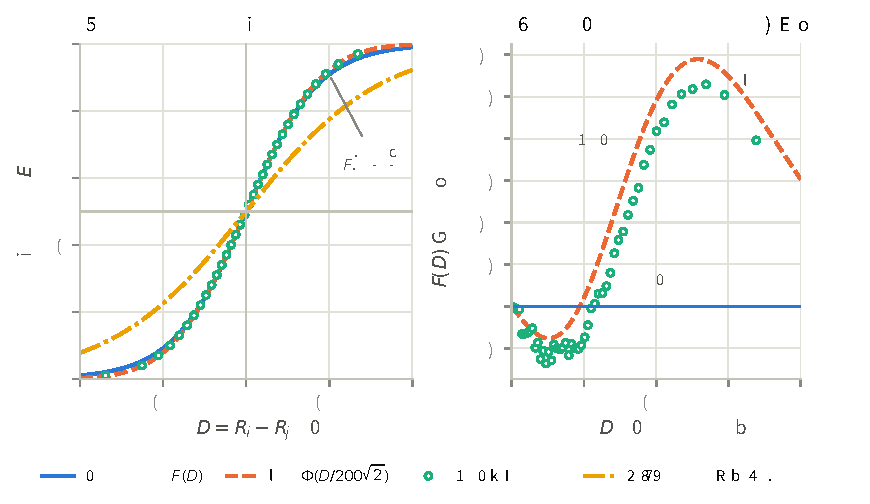
\includegraphics[width=\linewidth]{ch1/1a_curves.pdf}
  \caption{四种“评分差 $\to$ 期望得分”换算。(a) Elo 逻辑斯蒂曲线、单人表现标准差 200 的正态曲线、FIDE 等级分条例（2024 年 3 月 1 日起施行）8.1.1 换算表，以及 Glicko 在双方评分偏差 RD$=350$（未定级）时的预测式；(b) 正态曲线和 FIDE 表与逻辑斯蒂曲线之差。前三者差别不足 1.5 个百分点，FIDE 表贴近正态曲线；评分不确定时，Glicko 把预测明显拉向 50\%。纯解析计算。}
  \label{fig:1a-curves}
\end{figure}

\Cref{eq:1a-latent} 有三处明显的简化，后来几十年的评分研究基本就是逐条放松它们：（1）只有两个人、只有输赢——团队、多人名次和平局怎么办；（2）$s_i$ 固定且已知——估计有多不确定、实力随时间怎样变；（3）一个标量就能概括实力——存在“石头剪刀布”式克制时怎么办。匹配研究则多出第四个问题：在知道 $R_i$ 而不知道 $s_i$ 的前提下，应该优化什么目标。

\begin{keybox}
\begin{itemize}
  \item 评分是推断（估计 $s_i$），匹配是决策（选对手、分队）。“控胜率”若存在，只能在匹配层。
  \item 主流评分模型都基于“实力 + 随机表现”的潜变量框架；正态与逻辑斯蒂两种曲线相差不足 1.5 个百分点。
  \item FIDE 现行换算表仍是正态曲线（本项目逐格核对），400 分只是刻度：分差 400 对应约 90.9\% 的期望得分。
\end{itemize}
\end{keybox}

\section{评分模型的谱系：从成对比较到贝叶斯滤波}\label{sec:1a-models}

\Cref{fig:1a-timeline} 把本章引用的主要文献按年份排开。评分研究的主线很清楚：1920—1950 年代的心理测量学提供了成对比较模型；Elo 在 1950 年代末把它变成国际象棋的在线记分规则；1990 年代末起，Glickman 和微软研究院先后引入贝叶斯不确定性、团队与多人名次；2010 年代后期开始，研究者一方面把更多行为数据放进模型（TrueSkill 2），另一方面回头严格分析 Elo 本身的统计性质和一维评分的边界。

\begin{figure}[htbp]
  \centering
  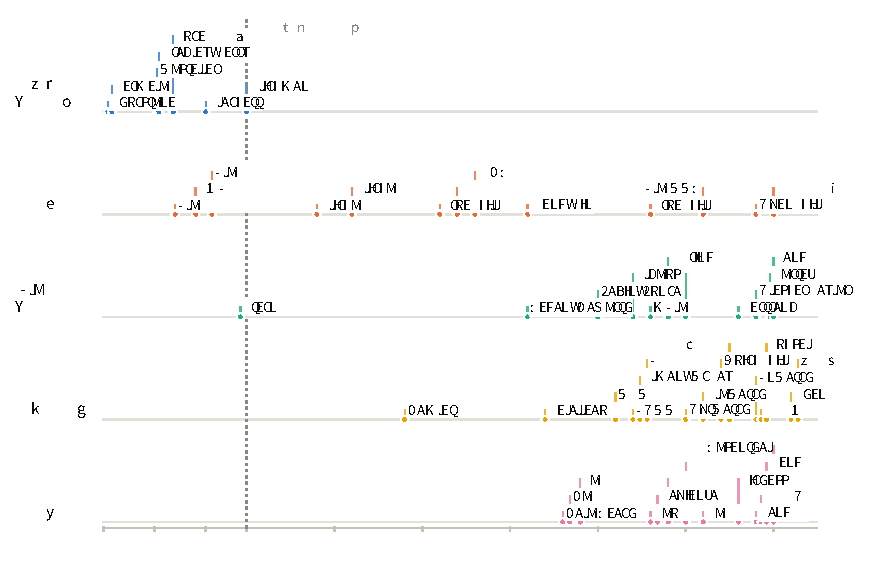
\includegraphics[width=\linewidth]{ch1/1a_timeline.pdf}
  \caption{评分模型与匹配机制研究的时间线。每个点是本章引用的一篇文献或一个标志性事件，年份取正式发表年（预印本取首次公开年）。1995 年后横轴放大约 7 倍：近十年的论文集中在匹配机制、Elo 理论和游戏实证三条线上。}
  \label{fig:1a-timeline}
\end{figure}

\subsection{成对比较：Thurstone、Zermelo、Bradley–Terry 与 Luce}\label{sec:1a-paired}

成对比较（paired comparison）研究的是“两两比较的结果如何还原成一个排序”。Thurstone 1927 年提出“比较判断律”：被试对刺激 $i$ 的感受是一个正态随机量，比较两刺激时取感受较大者；在各刺激方差相同、彼此不相关的第五种情形下，比较概率就是\cref{eq:1a-thurstone}\cite{thurstone1927law}\tagLit。Mosteller 1951 年给出了该情形下刻度值的最小二乘解法\cite{mosteller1951remarks}\tagLit，后人把这一组合称为 Thurstone–Mosteller 模型。

逻辑斯蒂一支更早出现在棋类中。Zermelo 1929 年的论文题目就是“把锦标赛成绩的计算写成概率论中的极大值问题”，他用今天称为 Bradley–Terry 的模型从循环赛结果推算棋手实力\cite{zermelo1929berechnung}\tagLit\needcheck[；本次只核对了题录，未重读德文原文]。Bradley 与 Terry 1952 年独立提出
\begin{equation}\label{eq:1a-bt}
  \Prob(i\ \text{胜}\ j) = \frac{\pi_i}{\pi_i+\pi_j} = \frac{1}{1+e^{-(\theta_i-\theta_j)}},\qquad \theta_i=\ln\pi_i ,
\end{equation}
用于不完全区组设计中的排序分析\cite{bradley1952rank}\tagLit。Luce 1959 年的选择公理把它推广到从集合 $S$ 中选一项：
\begin{equation}\label{eq:1a-luce}
  \Prob(i \mid S) = \frac{w_i}{\sum_{j\in S} w_j},
\end{equation}
即“选 $i$ 而不选 $j$ 的相对几率与集合里还有谁无关”（无关选项独立性）\cite{luce1959individual}\tagLit。Plackett 1975 年把逐个挑出第一名、第二名……的过程连乘起来，得到对整个名次排列 $\pi$ 的概率
\begin{equation}\label{eq:1a-pl}
  \Prob(\pi) = \prod_{k=1}^{N} \frac{w_{\pi(k)}}{\sum_{m=k}^{N} w_{\pi(m)}} ,
\end{equation}
后称 Plackett–Luce 模型\cite{plackett1975analysis}\tagLit。它是 8 人名次类游戏（自由混战、大逃杀、自走棋）最自然的统计模型：一局 $N=8$ 的名次相当于连续 7 次“从剩下的人里选出最强者”。

这些模型都是\emph{静态}的：$s_i$ 不随时间变，估计时把全部数据一起做极大似然。游戏和棋类需要的是\emph{在线}版本：每下一局就更新一次，且允许实力变化。Elo 系统正是这样一个在线估计器。

\subsection{Elo：把成对比较变成在线记分}\label{sec:1a-elo}

\paragraph{历史。}据 Glickman 的综述，第一个给出数值评分的国际象棋系统是 Anton Hoesslinger 1948 年在德国提出的 Ingo 系统；1950 年代美国棋联（USCF）用过 Ken Harkness 设计的系统，英国棋联用过 Richard Clarke 的系统。这些系统与棋手的主观排名大致吻合，但缺乏统计基础，例如在 Harkness 系统里，一个人可以在比赛中全输却仍然涨分。USCF 于 1960 年改用 Arpad Elo 的系统，FIDE 于 1970 年采用\cite{glickman1995comprehensive}\tagLit；Elo 本人 1978 年出版专著系统阐述这一方法\cite{elo1978rating}\tagLit。TrueSkill 论文给出的年份与此一致：Elo 1959 年提出该系统，FIDE 1970 年采用\cite{herbrich2006trueskill}\tagLit。

\paragraph{公式。}Elo 系统把\cref{eq:1a-latent} 中的 $s_i$ 换成当前评分 $R_i$，用曲线 $\Elogit$ 算出期望得分 $E_{ij}=\Elogit(R_i-R_j)$，赛后按“实际减期望”修正：
\begin{equation}\label{eq:1a-elo-update}
  R_i \leftarrow R_i + \Kf\Big(S_i - \sum_{j} E_{ij}\Big),
\end{equation}
其中 $S_i$ 是一个比赛周期（例如一次锦标赛）内的总得分（胜 1、和 0.5、负 0），求和遍历该周期的所有对手。双方 $\Kf$ 相同时，一局里一方涨多少、另一方就跌多少，整个分池的总分守恒。

\paragraph{两种读法。}$\Kf$ 有两种直观解释。第一种来自 Glickman：\cref{eq:1a-elo-update} 近似于“赛前评分”和“本次比赛表现分”的加权平均。对一次 4 轮的比赛，$\Kf=32$ 相当于给旧评分 94.7\%、给本次表现 5.3\% 的权重；$\Kf=24$ 对应 96.2\% 与 3.8\%，$\Kf=16$ 对应 97.5\% 与 2.5\%\cite{glickman1995comprehensive}\tagLit。换句话说，Elo 评分是历史表现的一个指数加权移动平均，越近的比赛权重越大。第二种读法来自统计学习：\cref{eq:1a-elo-update} 恰好是对 Bradley–Terry 对数似然做一步随机梯度上升（推导见下框），$\Kf$ 是学习率乘以常数 $\cElo$。Szczecinski 与 Djebbi\cite{szczecinski2019understanding}、Olesker-Taylor 与 Zanetti\cite{oleskertaylor2024analysis}、Tang 等\cite{tang2025elo} 都以这一等价为出发点\tagLit；第四章从训练模型的角度详细讨论它（\cref{ch:ml}）。

\begin{derivbox}[Elo 更新即随机梯度上升]
设一局只有 $i$、$j$ 两人，$y\in\{0,1\}$ 表示 $i$ 是否获胜，$E=\Elogit(R_i-R_j)$。单局对数似然为
$\ell = y\ln E + (1-y)\ln(1-E)$。由 $\Elogit'(x)=\cElo\,\Elogit(x)\big(1-\Elogit(x)\big)$ 得
\[
  \frac{\partial \ell}{\partial R_i} = \frac{y}{E}\,\cElo E(1-E) - \frac{1-y}{1-E}\,\cElo E(1-E) = \cElo\,(y-E).
\]
以步长 $\eta$ 做一步梯度上升：$R_i \leftarrow R_i + \eta\,\cElo\,(y-E)$。令 $\Kf=\eta\,\cElo$ 即得\cref{eq:1a-elo-update}；对 $R_j$ 的梯度恰为相反数，所以更新是零和的。$\Kf$ 越大，跟踪实力变化越快，但评分围绕实力的随机抖动也越大。\tagOwn
\end{derivbox}

\paragraph{现行规则。}FIDE 现行等级分条例（2024 年 3 月 1 日起施行）规定：新进入等级分表的棋手在完成至少 30 局之前 $\Kf=40$；18 岁生日所在年年底之前且等级分低于 2300 的棋手 $\Kf=40$；等级分低于 2400 时 $\Kf=20$；一旦公布等级分达到 2400，此后永久 $\Kf=10$，即使再跌破 2400；若一个评分周期内局数 $n$ 与 $\Kf$ 之积超过 700，则把 $\Kf$ 降到使 $\Kf n\le 700$ 的最大整数。自 2025 年 10 月 1 日起，“400 分规则”（分差超过 400 按 400 计）只适用于等级分低于 2650 的棋手\cite{fide2024rating}\tagOff。TrueSkill 论文做对照实验时使用的高斯版 Elo 取 $\alpha=0.07$，作者注明这相当于 Elo 刻度上 $\Kf=24$，“被认为是良好而稳定的动态”\cite{herbrich2006trueskill}\tagLit。

\paragraph{已知问题之一：用估计值做预测会过度自信。}\Cref{eq:1a-elo-curve} 描述的是\emph{真实实力}之间的关系，而系统手里只有带误差的评分。Glickman 分析了 1991—1993 年间 8300 多局 USCF 比赛，发现按公布评分算出的期望得分系统性地高估了高分一方的实际得分。他的解释是：对手评分有误差时，对“对手真实实力”的期望得分取平均，结果小于把评分直接代入公式；例如真实实力 1900 的棋手遇到公布评分 1700、但真实实力一半时间是 1600 一半时间是 1800 的对手，代入公式得 0.76，实际平均只有 $(0.64+0.85)/2=0.745$\cite{glickman1995comprehensive}\tagLit。三十年后，Szczecinski 把同一现象写成定理：由于估计噪声，“用于排名的模型”和“用于预测的模型”必须解耦，预测时的有效刻度要比排名刻度更平；他用六年的 FIFA 男足排名检验，发现绝大多数国家队的评分其实尚未收敛\cite{szczecinski2026new}\tagLit。这一点直接关系到第二章：游戏里“系统预测胜率 $E$”和“真实单局胜率 $p$”不是一回事（\cref{ch:winrate}）。

\paragraph{已知问题之二：封闭分池会通缩。}Glickman 把通缩的条件说得很清楚：玩家的平均实力随时间上升，而评分系统又不会凭空加分。满足这两个条件时，实力不变的老玩家会不断输分给正在进步、但评分偏低的新玩家。USCF 在 1970 年代中期观察到平均评分下滑，先后尝试过“奖励分”（bonus points）和“反馈分”（feedback points），1980 年代中期因过度补偿而取消，1980 年代后期改设“评分地板”\cite{glickman1995comprehensive}\tagLit。FIDE 在 2023 年公开承认过去十年的若干改动造成了通缩，提出对 2000 分以下（约占全部注册棋手 85\%）的棋手一次性加分 $0.4\times(2000-R)$，并把最低等级分从 1000 提到 1400、恢复 400 分规则\cite{fide2023seeks}\tagOff；2024 年施行的条例只公布 1400 分及以上的等级分\cite{fide2024rating}\tagOff。游戏中的“赛季重置”“段位保护”“保底分”可以看作同一问题的工程补丁。

\paragraph{已知问题之三：高端是否通胀。}与通缩相反，国际象棋顶端常被怀疑通胀（今天的 2700 不如过去的 2700）。Regan 与 Haworth 绕开胜负，用高深度引擎评估每步棋的质量，拟合出“内在评分”，结论是不同年代同一等级分对应的走子质量基本不变，“几乎没有评分通胀”\cite{regan2011intrinsic}\tagLit。TrueSkill Through Time 对 150 年国际象棋数据的回溯则发现整体棋力在上升\cite{dangauthier2007trueskill}\tagLit；两者并不矛盾：前者检验评分刻度是否漂移，后者估计不同年代的绝对水平。

\subsection{Glicko 与 Glicko-2：给评分加上误差棒}\label{sec:1a-glicko}

Glickman 用一个例子说明 Elo 的缺陷：两名 1700 分的棋手对局，一人刚从多年休赛中回来，另一人每周都下棋；在 USCF 的 Elo 下胜者涨 16 分、负者跌 16 分，但直觉上回归者的 1700 本来就不可信，他赢了应该涨得更多，而常客的 1700 已经测得很准，输给一个评分不可信的人不该跌太多\cite{glickman2016glicko}\tagLit。Glicko 系统由此给每人两个数：评分 $r$ 和评分偏差（rating deviation, RD），后者是 $r$ 的标准差。其完整推导是一个动态成对比较的状态空间模型\cite{glickman1999parameter}\tagLit；公开的计算步骤如下\cite{glickman2016glicko}\tagLit。

一个评分周期开始时，未定级玩家取 $r=1500$、RD$=350$；其他玩家的 RD 按休赛时间增大，$\mathrm{RD}\leftarrow\min\big(\sqrt{\mathrm{RD}^2+c^2},\,350\big)$。Glickman 举例说，若希望一个 RD$=50$ 的常客在 30 个评分周期不下棋后回到 350，则 $c=\sqrt{(350^2-50^2)/30}\approx 63.2$。周期结束时，对手 $j=1,\dots,m$ 的得分 $s_j$ 按下式更新：
\begin{equation}\label{eq:1a-glicko}
\begin{gathered}
  q=\frac{\ln 10}{400},\qquad g(\mathrm{RD})=\frac{1}{\sqrt{1+3q^2\mathrm{RD}^2/\pi^2}},\qquad
  E_j=\frac{1}{1+10^{-g(\mathrm{RD}_j)(r-r_j)/400}},\\
  d^2=\Big[q^2\sum_j g(\mathrm{RD}_j)^2E_j(1-E_j)\Big]^{-1},\qquad
  r' = r + \frac{q}{1/\mathrm{RD}^2+1/d^2}\sum_j g(\mathrm{RD}_j)(s_j-E_j),\qquad
  \mathrm{RD}'=\Big(\frac{1}{\mathrm{RD}^2}+\frac{1}{d^2}\Big)^{-1/2}.
\end{gathered}
\end{equation}
三处变化值得注意。第一，$g(\mathrm{RD}_j)<1$ 把对手不确定时的期望得分拉向 0.5，这正是 Glickman 1995 年观察到的过度自信问题的修正。预测两人对局时，Glicko 用 $g\big(\sqrt{\mathrm{RD}_i^2+\mathrm{RD}_j^2}\big)$ 折减分差，\cref{fig:1a-curves}(a) 中的点划线就是双方 RD$=350$ 时的预测。第二，步长 $q/(1/\mathrm{RD}^2+1/d^2)$ 随自己的 RD 增大，相当于一个自动调节的 $\Kf$：新号和回归者涨跌快，老玩家涨跌慢。第三，更新不再零和，双方的变化量由各自的 RD 决定。Glickman 建议每个评分周期平均 5—10 局；FICS 国际象棋服务器采用逐局更新的版本\cite{glickman2016glicko}\tagLit。

Glicko-2 再增加一个“波动率”$\sigma$，描述实力本身变化的剧烈程度：长期稳定后突然打出远超预期的成绩，$\sigma$ 变大，RD 随之放大，评分就能更快追上\cite{glickman2001dynamic}\tagLit。计算时先换到内部刻度 $\mu=(r-1500)/173.7178$、$\phi=\mathrm{RD}/173.7178$，算出仅由本周期结果给出的方差 $v$ 和“表现改进量”$\Delta$，用 Illinois 算法（一种试位法）解出新的 $\sigma'$，再更新
\begin{equation}\label{eq:1a-glicko2}
  \phi^{*}=\sqrt{\phi^2+\sigma'^2},\qquad
  \phi'=\Big(\frac{1}{\phi^{*2}}+\frac{1}{v}\Big)^{-1/2},\qquad
  \mu'=\mu+\phi'^2\sum_j g(\phi_j)\big(s_j-E(\mu,\mu_j,\phi_j)\big).
\end{equation}
系统常数 $\tau$ 约束波动率的变化，Glickman 建议取 0.3—1.2，并建议每个周期平均至少 10—15 局；新玩家的初始波动率取 0.06。他给的算例里，一名 1500 分、RD$=200$ 的玩家一胜两负后变为 1464.06 分、RD$=151.52$\cite{glickman2022example}\tagLit。Glicko-2 的“波动率”可以理解为对实力波动的一个粗糙建模，第三章讨论的“上头”与状态起伏正是这类波动（\cref{ch:streaks}）。Lichess 使用 Glicko-2 评分（Chowdhary 等的分析即以其为技能指标）\cite{chowdhary2023quantifying}\tagLit；CS:GO 被认为使用一个未公开的 Glicko-2 变体，但这一说法来自社区资料\cite{bober2024skill}\tagCom。

\subsection{TrueSkill：因子图上的团队、多人与平局}\label{sec:1a-trueskill}

TrueSkill 是为团队与多人在线游戏设计、并在 Xbox Live 上大规模部署的贝叶斯评分系统，作者称它是迄今最大规模的贝叶斯推断应用之一\cite{herbrich2006trueskill}\tagLit。它要解决 Elo 和 Glicko 都不处理的两个问题：比赛结果常常是团队的，而匹配需要个人评分；一局可能有两个以上的队伍，结果是一个名次排列而不是一胜一负。

\paragraph{模型。}每名玩家的实力有高斯先验 $s_i\sim\Normal(\mu_i,\sigma_i^2)$；一局中的表现 $p_i\sim\Normal(s_i,\beta^2)$；队伍 $j$ 的表现是成员表现之和 $t_j=\sum_{i\in A_j}p_i$；名次由队伍表现的大小决定。允许平局时，相邻名次要求 $t_{r(j)}>t_{r(j+1)}+\varepsilon$，平局要求 $|t_{r(j)}-t_{r(j+1)}|\le\varepsilon$，平局边际 $\varepsilon$ 由观测到的平局率反推：
\begin{equation}\label{eq:1a-ts-draw}
  \Prob(\text{平局}) = 2\,\Phi\!\left(\frac{\varepsilon}{\sqrt{n_1+n_2}\,\beta}\right)-1 ,
\end{equation}
$n_1,n_2$ 是比较的两队人数\cite{herbrich2006trueskill}\tagLit。推断在因子图上用近似消息传递（期望传播，矩匹配）完成，每局之后把后验近似为高斯，作为下一局的先验（“高斯密度滤波”）；作者报告其运行时间不超过简单 Elo 更新的两倍。对最常见的两人（或两队）一胜一负，后验可以写成闭式（推导见\cref{app:ch1a-ts}）：记 $c^2=2\beta^2+\sigma_{\mathrm w}^2+\sigma_{\mathrm l}^2$，$t=(\mu_{\mathrm w}-\mu_{\mathrm l})/c$，
\begin{equation}\label{eq:1a-ts-update}
  \mu_{\mathrm w}\leftarrow \mu_{\mathrm w}+\frac{\sigma_{\mathrm w}^2}{c}\,v\!\left(t,\tfrac{\varepsilon}{c}\right),\quad
  \mu_{\mathrm l}\leftarrow \mu_{\mathrm l}-\frac{\sigma_{\mathrm l}^2}{c}\,v\!\left(t,\tfrac{\varepsilon}{c}\right),\quad
  \sigma_k^2\leftarrow\sigma_k^2\Big[1-\frac{\sigma_k^2}{c^2}\,w\!\left(t,\tfrac{\varepsilon}{c}\right)\Big],
\end{equation}
其中 $v(t,a)=\varphi(t-a)/\Phi(t-a)$，$w(t,a)=v(t,a)\big(v(t,a)+t-a\big)$，$\varphi$ 为标准正态密度，下标 w、l 表示胜方与负方，$k\in\{\mathrm w,\mathrm l\}$。爆冷时 $t$ 为负，$v$ 很大，更新幅度也大；均势对局的更新最温和。与 Glicko 一样，步长正比于自己的方差 $\sigma_k^2$。

\paragraph{匹配质量。}TrueSkill 用“平局概率”衡量一局是否势均力敌：两名玩家的匹配质量定义为 $\varepsilon\to0$ 时的平局概率与其可能最大值之比，
\begin{equation}\label{eq:1a-ts-quality}
  q_{\text{draw}} = \sqrt{\frac{2\beta^2}{2\beta^2+\sigma_i^2+\sigma_j^2}}\;
  \exp\!\left(-\frac{(\mu_i-\mu_j)^2}{2\,(2\beta^2+\sigma_i^2+\sigma_j^2)}\right).
\end{equation}
作者特别指出，一局的质量由其结果的不可预测性决定，所以“匹配的目标与寻找信息量最大的对局是一致的”\cite{herbrich2006trueskill}\tagLit。\Cref{sec:1a-mm-info} 会回到这一点。

\paragraph{部署参数。}Xbox 360 Live 上的 TrueSkill 取先验 $\mu_0=25$、$\sigma_0=25/3$，表现噪声 $\beta=\sigma_0/2$，每局附加的动态方差 $(\sigma_0/100)^2$；排行榜显示保守估计 $\mu-3\sigma$（约 1\% 下分位数），保证榜首是“有把握地强”的玩家。系统每天处理数十万局\cite{herbrich2006trueskill}\tagLit。

\paragraph{实证结果。}作者用 Bungie 提供的《光环 2》（Halo 2）公测数据比较 TrueSkill 与高斯版 Elo（团队赛用“对决启发式”：每人与对方每人两两比较后取平均更新）。\Cref{tab:1a-halo2} 列出预测错误率。作者提醒，有匹配器参与时，这一指标很难解读：取决于玩家的真实实力，能达到的最小错误率可能高达 50\%。为此他们设计了“挑战集”：每个系统挑出自认为最势均力敌的 20\% 对局交给对方预测。在挑战集上 TrueSkill 全面占优；在全集上，4 对 4 的 Small Teams 模式中 Elo 略好。作者还报告了一个重要的反例：按匹配质量排序时，TrueSkill 在 Small Teams 模式不如 Elo，“可能是因为这一模式多为夺旗玩法，违反了团队表现可加的假设”\cite{herbrich2006trueskill}\tagLit。这是 TrueSkill 作者自己承认“团队实力 = 成员之和”可能失效，比 TrueSkill 2 的车队数据（\cref{sec:1a-ts2}）早了 12 年。收敛速度方面，作者展示了 8 人自由混战中两名高分玩家的收敛轨迹：TrueSkill 约 10 局收敛，信息论下限约为 $\log n/\log 8\approx5$ 局，而 Elo 收敛缓慢；需要注意这只是两名示例玩家，不是平均值。在过滤掉低质量对局的 1 对 1 模式中，即使局数很少的玩家也大多得到了“公平”的对局（获胜概率在 35\%—65\% 之间）。

\begin{table}[htbp]
  \centering\small
  \caption{《光环 2》公测数据上的预测错误率（\%，越低越好）。“挑战集”为对方系统认为最势均力敌的 20\% 对局。数据摘自 Herbrich 等\cite{herbrich2006trueskill}，Weng–Lin 一列摘自 Weng 与 Lin\cite{weng2011bayesian}（Bradley–Terry 全配对算法，同一数据、同一指标）。}
  \label{tab:1a-halo2}
  \begin{tabular}{lcccccc}
    \toprule
    模式 & 每队人数 & Elo（全集） & TrueSkill（全集） & Weng–Lin（全集） & Elo（挑战集） & TrueSkill（挑战集）\\
    \midrule
    Free for All & 8 人各自为战 & 32.14 & 30.82 & 30.59 & 38.30 & 35.64\\
    Small Teams & 4 对 4 & 34.92 & 35.23 & 33.97 & 42.55 & 37.17\\
    Head to Head & 1 对 1 & 33.24 & 32.44 & 32.53 & 40.57 & 30.83\\
    Large Teams & 8 对 8 & 39.49 & 38.15 & 37.30 & 44.12 & 29.94\\
    \bottomrule
  \end{tabular}
\end{table}

\paragraph{作者观察到的反馈回路。}论文最后记录了 Xbox Live 上的三个现象：不同游戏的“有效技能层级数”差别很大，运气成分大的游戏技能分布窄；玩家把显示的评分当作奖惩，有人为保分停玩、挑对手或作弊；新玩家起初连续输球会把整体评分分布压到先验之下，一次评分重置并收紧匹配后这一现象消失\cite{herbrich2006trueskill}\tagLit。最后一条与 Glickman 描述的通缩机制是同一回事。

\subsection{全历史方法与解析近似：TTT、WHR 与 Weng–Lin}\label{sec:1a-smoothing}

Elo、Glicko、TrueSkill 都只向前传递信息：一局结束后更新参与者，不回头修正过去。TrueSkill 2 的作者用一个例子说明这样做会丢信息：6 名初始相同的玩家依次进行 A 胜 B、C 胜 D、E 胜 F、B 胜 C、D 胜 E 五局，逐局更新会让 B 与 D、C 与 E 的评分完全相同，而把五局放在一起看，顺序显然应是 A$>$B$>$C$>$D$>$E$>$F\cite{minka2018trueskill}\tagLit。

TrueSkill Through Time（TTT）把每名玩家每年的实力当作一个变量，前后年份用高斯随机游走相连，在整个时间序列上做期望传播平滑而不是滤波；它还给每名棋手估计一个“逼和能力”（个人平局边际）。作者用 ChessBase 约 350 万局、跨度 150 年的数据重建了历史棋手的实力曲线，结论是整体棋力在 150 年间上升，而且建模个人平局边际能明显提高预测力\cite{dangauthier2007trueskill}\tagLit。该方法十多年来没有主流语言的实现，2025 年 Landfried 与 Mocskos 发布了 Julia、Python 和 R 版本，并用 ATP 男子网球数据估计历史球员的学习曲线\cite{landfried2025trueskill}\tagLit。

Coulom 的全历史评分（Whole-History Rating, WHR）同样基于动态 Bradley–Terry 模型，用维纳过程描述实力漂移，但不做近似消息传递，而是直接对所有玩家的整段评分历史求精确的最大后验估计\cite{coulom2008whole}\tagLit。他在 KGS 围棋服务器 2000—2007 年的数据（21.3 万名玩家、1080 万局）上，用 2005 年 5 月之前的 72.7 万局调参、之后的 233 万局测试，预测正确率依次为：Elo 55.12\%、Glicko 55.52\%、TrueSkill 55.54\%、Bayeselo 55.67\%、指数衰减历史 55.70\%、WHR 55.79\%。WHR 最好，但所有方法相差不到 0.7 个百分点，而 WHR 在训练集上耗时 252 秒，Elo 只要 0.4 秒。

Weng 与 Lin 走的是另一条路：用 Woodroofe 版本的 Stein 恒等式推出团队、多队排名的解析更新式，不需要 TrueSkill 的迭代消息传递，涵盖 Bradley–Terry、Thurstone–Mosteller 和 Plackett–Luce 三类模型\cite{weng2011bayesian}\tagLit。以 Bradley–Terry 全配对版本为例，队伍 $i$ 的实力均值与方差取成员之和 $\mu_i=\sum_j\mu_{ij}$、$\sigma_i^2=\sum_j\sigma_{ij}^2$，与每支对手队 $q$ 比较：
\begin{equation}\label{eq:1a-wenglin}
  c_{iq}=\sqrt{\sigma_i^2+\sigma_q^2+2\beta^2},\quad
  \hat p_{iq}=\frac{e^{\mu_i/c_{iq}}}{e^{\mu_i/c_{iq}}+e^{\mu_q/c_{iq}}},\quad
  \Omega_i=\sum_{q\ne i}\frac{\sigma_i^2}{c_{iq}}\big(s_{iq}-\hat p_{iq}\big),
\end{equation}
$s_{iq}$ 为实际结果（胜 1、平 1/2、负 0），成员均值按 $\mu_{ij}\leftarrow\mu_{ij}+(\sigma_{ij}^2/\sigma_i^2)\,\Omega_i$ 分摊，方差按类似的乘法因子收缩。在同一份《光环 2》数据上，它的错误率与 TrueSkill 相当（\cref{tab:1a-halo2}），F\# 实现跑完 Free for All 数据只需 1.2 秒（TrueSkill 13 秒），代码不到 100 行（TrueSkill 超过 500 行）。开源库 OpenSkill 实现了 Weng–Lin 的各算法；作者自己报告的一个 Overwatch 小数据集上，TrueSkill 的预测准确率反而更高（92.44\% 对 87.56\%），OpenSkill 的优势在速度（0.97 秒对 3.41 秒）\cite{joshy2024openskill}\tagLit。

\subsection{TrueSkill 2：先找出假设错在哪，再改模型}\label{sec:1a-ts2}

TrueSkill 2 是微软研究院与《战争机器》开发商 The Coalition 合作的技术报告（未经同行评审），也是目前公开文献中对一款商业射击游戏评分系统描述最完整的一份\cite{minka2018trueskill}\tagLit。作者先列出游戏工作室的七项要求：支持任意队伍数和人数；无论打了多少局，评分都必须还能变化；兼容只接受单个数字的现有匹配器；激励相容（不能让玩家为刷分而损害队友，例如若按自我治疗次数加分，玩家就会故意受伤）；训练数据需求小；计算成本低；上线后不需要人工调参。

报告把经典 TrueSkill 的假设归纳为五条：表现是实力的带噪样本；队伍表现是按上场时间加权的成员表现之和；只用胜负/平局，不用比分；实力做无偏随机游走；各游戏模式的实力相互独立。TrueSkill 2 对每一条都做了修改，而且每项修改都由一个“指标”驱动：把玩家按某个特征分组，比较实际胜率与模型预期胜率，出现系统性偏差才改模型（作者称为“指标驱动建模”）。数据是 343 Industries 提供的《光环 5》自 2015 年发售以来的全部对局：用发售后的 2300 万局训练，其后的 300 万局测试。

\begin{enumerate}
  \item \textbf{车队偏移。}按玩家所在车队（预先组队的朋友）人数分组，经典 TrueSkill 的预期胜率与实际胜率相差悬殊：4 人车队实际 57\%、预期 52\%；8 人车队实际 68\%、预期 49\%；10 人以上实际 89\%、预期 67\%（\cref{fig:1a-squad}）。作者的结论是“关于车队的假设是错的：车队的实力应大于成员之和，且效应随车队规模增大”，并提到《光环 5》和《战争机器 4》的部分模式因此禁止大车队，而另一些游戏强制车队只匹配车队，代价是缩小匹配池。TrueSkill 2 的修正很简单：表现改为 $p_i\sim\Normal\big(s_i+\mathrm{squadOffset}(\text{车队人数}),\beta^2\big)$，单人偏移固定为 0。
  \item \textbf{经验效应。}按已玩局数分组，新玩家实际胜率 45\%，模型预期 49\%：玩家在最初几局进步最快。修正是让随机游走带一个随局数变化的正漂移（前 200 局各有一个参数），作者描述为“每局之后无论胜负都给一点小的加分”。这一修正还自动解释了另一现象：玩家久未上线后胜率下降。
  \item \textbf{个人统计。}按上一局每分钟击杀数分组，击杀率最低组实际胜率 43\%、预期 48\%，最高组实际 59\%、预期 50\%。TrueSkill 2 用截断高斯模型让击杀、死亡数依赖于表现变量，并强制单调，以免玩家为凑某个数字而改变打法。
  \item \textbf{中途退出}按投降处理，无论结果都按输更新；\textbf{跨模式相关}（两个模式的评分相关系数约 0.6）通过一个共同的“基础实力”加模式偏移实现。
\end{enumerate}

这些修改合起来，把测试集上的预测准确率从 52\% 提到 68\%。这里的“准确率”指预测获胜队伍（或首名平局）是否正确，可选项为队伍数加一，不是二选一的抛硬币\cite{minka2018trueskill}\tagLit。报告还透露了几条有用的设计信息：《光环 5》的典型参数为新玩家实力先验均值 3、方差 1.6，每局随机游走标准差 $10^{-3}$，表现噪声 $\beta=1$（固定刻度）；模型故意不使用“几点上线”“和谁组队”这类与实力相关的信息，因为“激励应当是把游戏打好，而不是挑特定时间、和特定队友排队”。《战争机器 4》自 2016 年发售起使用 TrueSkill 2：实时做在线更新，每个排位赛季开始前用 TrueSkill Through Time 对全部历史批量重算；社交和合作模式中的电脑机器人按难度各当作一名实力固定的“玩家”，为人类评分提供固定参照\cite{minka2018trueskill}\tagLit。

\begin{figure}[htbp]
  \centering
  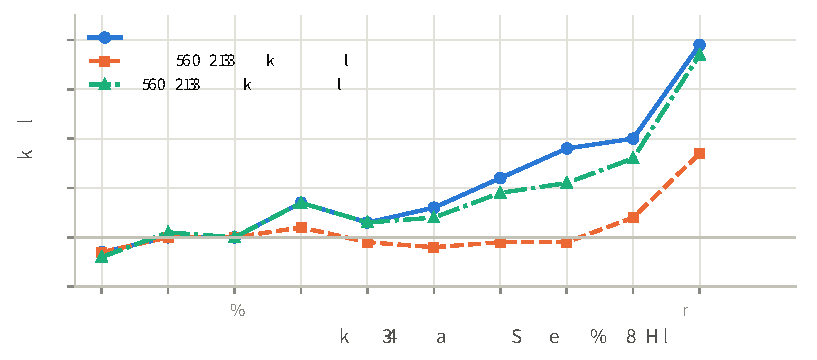
\includegraphics[width=\linewidth]{ch1/1a_squad.pdf}
  \caption{《光环 5》测试集中车队人数与胜率。经典 TrueSkill 按“队伍实力 = 成员之和”给出的预期胜率在 4 人以上车队明显偏低；加入车队偏移后，TrueSkill 2 的预期接近实际。数据逐格抄自 Minka 等\cite{minka2018trueskill} 第 6 节两张表（原文第二张表中 6 人车队实际胜率印作 55，此处取第一张表的 56）。}
  \label{fig:1a-squad}
\end{figure}

\subsection{多人名次：Plackett–Luce 与 Elo-MMR}\label{sec:1a-ffa}

8 人一局、只看名次的游戏（自由混战、大逃杀、自走棋、编程竞赛）有三种建模办法。第一种是 Plackett–Luce（\cref{eq:1a-pl}），Weng–Lin 给出了它的在线解析更新。第二种是 TrueSkill 的做法：把 $N$ 名玩家的表现排序，因子图只连接相邻名次，共 $N-1$ 个比较因子，《光环 2》的 8 人自由混战就是这样处理的\cite{herbrich2006trueskill}\tagLit。第三种是 Ebtekar 与 Liu 的 Elo-MMR：每轮先根据名次和他人当前评分估计每名选手本轮的“表现”，再把表现当作观测更新信念；表现分布取逻辑斯蒂以获得稳健性\cite{ebtekar2021elo}\tagLit。名字里的 MMR 指 Massive（大规模，计算量线性）、Monotonic（单调，即激励相容：想提高评分的人永远不会想故意表现差）、Robust（稳健，单轮评分变化有界）。作者证明了这些性质；处理 Codeforces 全部 30 多万名有评分的用户和 1000 场比赛不到一分钟，比 Codeforces 现行系统快一个数量级，预测精度相当或更好。他们指出，TrueSkill 被认为满足前两条但没有证明，且不满足稳健性。

这三种模型都可以直接用于《炉石传说》酒馆战棋一类的 8 人名次游戏，但公开文献中没有任何一篇用酒馆战棋的真实数据检验过它们（\cref{sec:1a-games-hs}）。对这类游戏，“胜率”本身也要重新定义：第二章讨论了“前四”“第一”等不同定义下的基准率（\cref{ch:winrate}）。

\subsection{非传递性：一维评分的边界}\label{sec:1a-intransitive}

\Cref{eq:1a-latent} 隐含了传递性：若 A 大概率胜 B、B 大概率胜 C，则 A 必然大概率胜 C。Balduzzi 等指出，Elo 在“石头剪刀布”式的循环博弈中没有任何预测力，还可以被操纵：往数据里加入大量“它能打赢的对手”的副本，就能抬高某个体的评分\cite{balduzzi2018reevaluating}\tagLit。他们用组合 Hodge 分解把胜负矩阵分成传递分量（可由一维评分表示）和循环分量，提出多维 Elo（mElo）：
\begin{equation}\label{eq:1a-melo}
  \hat p_{ij}=\sigma\!\big(r_i-r_j+\mathbf c_i^{\top}\,\Omega\,\mathbf c_j\big),\qquad
  \Omega=\sum_{k}\big(\mathbf e_{2k-1}\mathbf e_{2k}^{\top}-\mathbf e_{2k}\mathbf e_{2k-1}^{\top}\big),
\end{equation}
其中 $\mathbf c_i$ 是 $2k$ 维的“克制向量”，$\Omega$ 反对称，所以 $\mathbf c_i^\top\Omega\mathbf c_j=-\mathbf c_j^\top\Omega\mathbf c_i$。在 7 个 AlphaGo 变体加 Zen 的对战数据上，最简单的二维版本把预测误差（与经验胜率矩阵之差的 Frobenius 范数）从 Elo 的 0.85 降到 0.35，并纠正了 Elo 判错的几组三元克制关系。Czarnecki 等进一步论证，井字棋、围棋、星际争霸 II 等真实游戏的策略空间像一个“陀螺”：顶端（最强处）接近传递，中段循环最多\cite{czarnecki2020real}\tagLit。Bertrand 等证明，即使在很简单的传递博弈中，Elo 也可能提取不出正确的传递分量，并提出给每人两个数（实力与稳定性）的“圆盘排名”\cite{bertrand2023limitations}\tagLit。

反过来的证据同样重要。Tang、Wang 与 Jin 用似然比检验发现，多数真实对局数据集都显著偏离 Bradley–Terry 假设，也不平稳；但在胜率预测上，Elo 仍然常常胜过专门为非传递性设计的 mElo 等复杂模型\cite{tang2025elo}\tagLit。他们给出三个解释：Elo 可以看作在线梯度下降，在模型设定错误和非平稳时仍有“无悔”保证；真实对局数据很稀疏，复杂模型估不准；Elo 的预测精度与排名质量高度相关。对游戏而言，这意味着英雄、卡组、阵容造成的克制确实存在，单一 MMR 只是它们的投影；但在每对玩家只交手少数几次的天梯数据上，一维评分仍是合理的折中。

\subsection{Elo 的统计行为：近十年的理论结果}\label{sec:1a-theory}

尽管 Elo 使用了六十多年，严格分析它的工作直到近十年才多起来。Aldous 2017 年称之为“应用概率中被忽视的课题”\cite{aldous2017elo}\tagLit。他把 Elo 抽象为：胜方加 $\Upsilon(y_i-y_j)$、负方减同样的量，$\Upsilon$ 递减。若真实胜率函数为 $W$，则满足“平衡关系”
\begin{equation}\label{eq:1a-balance}
  \frac{\Upsilon(u)}{\Upsilon(-u)}=\frac{W(-u)}{W(u)}
\end{equation}
时，评分差等于实力差的那一刻，评分差的期望变化为零；常用的 $\Upsilon(u)=\delta\,W(-u)$（即 $\Kf\cdot(1-E)$）是一个解。Aldous 证明，在随机配对下评分过程有唯一的平稳分布，且从任意初值出发都收敛到它；但这一定理不说明平稳分布离真实实力有多近。于是他转向模拟：在三种实力随时间变化的模型下，评分误差来自“曲线选错”“滞后”和“噪声”三部分，滞后随 $\Kf$ 变小而增大，噪声随 $\Kf$ 变大而增大。他的结论是：在合理的实力变化模型下，无论打了多少局，预测胜率的典型误差都不会显著低于 10\%；若永远预测 50\%，误差为 15.9\%（实力标准差 0.5 个逻辑斯蒂单位）或 26.1\%（标准差 1）；要把误差减半，实力需要大约 150—200 局才发生显著变化。他追查了网上广为复制的“约 30 场后评分就会收敛到真实实力”的说法，没有找到任何来源或依据\cite{aldous2017elo}\tagLit。

另一条线是“动力学”（kinetic）模型：把大量玩家的评分分布看作一个随时间演化的密度。Jabin 与 Junca 提出了 Elo 的连续模型\cite{jabin2015continuous}，据 Aldous 及 Düring 等的转述，他们在一定假设下证明评分密度收敛到实力密度\tagLit\needcheck[；对 Jabin 与 Junca 结论的描述来自后续论文的转述]。Düring、Torregrossa 与 Wolfram 加入学习效应，推导出 Boltzmann 型和 Fokker–Planck 型方程\cite{during2019boltzmann}\tagLit；Düring、Fischer 与 Wolfram 再推广到表现可变的个人与团队\cite{during2022elo}\tagLit。

最近三年的结果把这些定性结论变成了定量的。Cortez 与 Tossounian 证明，随机配对下 Elo 评分过程以指数速率（在 2-Wasserstein 距离下且几乎必然）收敛到唯一平稳分布；平稳分布有有限的指数矩、支撑集是全空间，并在 $\Kf\to0$ 时以 $\sqrt{\Kf}$ 的速率收敛到真实实力\cite{cortez2026convergence}\tagLit。Olesker-Taylor 与 Zanetti 在 Bradley–Terry–Luce 模型下用马尔可夫链工具证明，对时间平均、并对评分设上下限的 Elo，其学习参数的速率可与最好的离线算法相比；他们还把“如何安排对局让 Elo 收敛最快”转化为图上“最快混合马尔可夫链”问题\cite{oleskertaylor2024analysis}\tagLit。Szczecinski 2026 年的半教程式论文给出了 $\Kf$ 与刻度如何同时决定收敛时间（约与 $\Kf$ 成反比）和收敛后估计方差（约与 $\Kf$ 成正比）的闭式结果\cite{szczecinski2026new}\tagLit；他与 Djebbi 此前指出，Elo 把平局记作半胜半负，隐含了一个特定的平局模型，并提出可调平局频率的 $\kappa$-Elo\cite{szczecinski2019understanding}\tagLit。2026 年还有工作尝试把每步棋的质量（而不只是胜负）纳入 Elo，以更快跟踪实力变化，同时证明其与传统 Elo 的偏差有界\cite{zhou2026accelerating}\tagLit。这些理论都在说同一件事：固定 $\Kf$ 的 Elo 永远在“追得快”和“抖得小”之间取舍，第二章和第四章分别从胜率和训练的角度给出这一取舍的具体数字（\cref{ch:winrate,ch:ml}）。

\Cref{tab:1a-models} 把本节讨论的模型汇总在一起，作为索引。

\begin{table}[htbp]
  \centering\small
  \caption{主要评分模型一览（摘要表；正文给出公式与证据）。}
  \label{tab:1a-models}
  \begin{tabularx}{\linewidth}{>{\raggedright\arraybackslash}p{2.3cm}>{\raggedright\arraybackslash}p{2.6cm}>{\raggedright\arraybackslash}X>{\raggedright\arraybackslash}X}
    \toprule
    模型（年份） & 胜负模型 & 相对前人修正了什么 & 已知局限或实证 \\
    \midrule
    Elo（1959/1978） & 正态或逻辑斯蒂 & 把成对比较变成在线更新 & 固定 $\Kf$；预测过度自信；封闭分池通缩 \\
    Glicko（1999） & 逻辑斯蒂 + 评分偏差 & 不确定性 RD，自动调步长 & 只处理两人；需要评分周期 \\
    Glicko-2（2001） & 同上 + 波动率 & 实力突变 & 同上；$\tau$ 需调 \\
    TrueSkill（2006） & 正态，队伍 = 成员之和 & 团队、多队、平局、匹配质量 & 夺旗模式中可加假设失效 \\
    TTT（2007）/WHR（2008） & 正态/动态 BT & 全历史平滑 & 计算量大；KGS 上各法差距 $<0.7$ 个百分点 \\
    Weng–Lin（2011） & BT、TM、PL & 解析更新，快 & 精度与 TrueSkill 相当 \\
    TrueSkill 2（2018） & 正态 + 个人统计 & 车队、经验、退出、跨模式 & 技术报告；《光环 5》准确率 52\%$\to$68\% \\
    Elo-MMR（2021） & 逻辑斯蒂表现 & 大规模名次赛、激励相容证明 & 未在游戏天梯上检验 \\
    mElo（2018）等 & BT + 循环分量 & 非传递性 & 稀疏数据上常不如 Elo \\
    \bottomrule
  \end{tabularx}
\end{table}

\begin{keybox}
\begin{itemize}
  \item 评分模型的演化是逐条放松“两人、固定实力、一维”这三个假设：Glicko 引入不确定性，TrueSkill 引入团队与多人，TTT/WHR 引入全历史平滑，mElo 处理非传递性，TrueSkill 2 把更多行为数据放进模型。
  \item 增益最大的往往不是换公式，而是修正错误假设：TrueSkill 2 在《光环 5》上把准确率从 52\% 提到 68\%，主要靠车队、经验和个人统计；而 KGS 围棋数据上 Elo、Glicko、TrueSkill、WHR 的差距不到 0.7 个百分点。
  \item 理论上，固定 $\Kf$ 的 Elo 收敛到一个围绕真实实力抖动的平稳分布，抖动随 $\sqrt{\Kf}$ 缩小；Aldous 的模拟表明预测误差很难低于 10\%，“30 场就收敛”的说法查无出处。
\end{itemize}
\end{keybox}

\section{匹配机制本身的研究}\label{sec:1a-mm}

评分研究问“这个人多强”，匹配研究问“给定一池正在排队的人，怎样配对、分队最好”。“最好”至少有四种含义：结果最难预测（公平）、对估计实力最有信息量、等待时间短、玩家留得住。前两者在 TrueSkill 的框架下是同一个目标；后两者则与公平存在真实的冲突。本节按这四个目标组织文献，最后讨论玩家对连胜连败的反应，因为“参与度优化”正是建立在这些反应之上。

\subsection{公平与信息量：同一个目标}\label{sec:1a-mm-info}

一局的结果若能提前猜到，它对估计双方实力几乎没有帮助；若胜率接近 50\%，结果的不确定性（二元熵）最大，单局的 Fisher 信息 $\cElo^2p(1-p)$ 也在 $p=1/2$ 时最大（\cref{ch:ml}）。TrueSkill 的匹配质量\cref{eq:1a-ts-quality} 把这一点做成了匹配准则\cite{herbrich2006trueskill}\tagLit。Bober-Irizar 等把“选哪两队对局”当作主动学习中的“采集函数”，在 2017—2022 年 HLTV 收录的 9929 场职业与半职业 CS:GO 比赛上比较：挑选“最可能平局”或“交叉熵最大”的对局，比随机挑选的预测准确率高 1—1.5 个百分点；有意思的是，直接用 TrueSkill 自带的匹配质量来挑，反而不如随机挑\cite{bober2024skill}\tagLit。另一方面，Yuksel 的模拟提醒，按分匹配并不总是对估计有利：在他的设定中，Elo、Glicko、TrueSkill 估计整个群体评分的误差，在随机配对下都比在按分匹配下更小，因为按分匹配让比较集中在相邻的人之间\cite{yuksel2024skill}\tagLit。

匹配还会反过来影响评估。TrueSkill 作者指出，有匹配器参与时，最好的系统预测错误率也可能接近 50\%\cite{herbrich2006trueskill}\tagLit；TrueSkill 2 因此改用“分组的实际胜率 vs 预期胜率”作为主要诊断工具\cite{minka2018trueskill}\tagLit。这是第二章“观察到的胜率接近五成不代表实力相同”的文献来源（\cref{ch:winrate}）。

\subsection{等多久：等待时间与匹配质量的在线权衡}\label{sec:1a-mm-wait}

理论计算机科学把“马上配一个差一点的，还是再等等”形式化为带延迟的最小代价完美匹配（min-cost perfect matching with delays, MPMD）。Emek、Kutten 与 Wattenhofer 以国际象棋、拼字游戏等在线对战平台的匹配为动机提出这一问题：请求在连续时间里到达一个度量空间中的点（例如评分），算法可以推迟配对，但总代价是“已配对请求之间的距离之和”加上“每个请求的等待时间之和”，
\begin{equation}\label{eq:1a-mpmd}
  \mathrm{cost}(M)=\sum_{(u,v)\in M} \mathrm{dist}(u,v) + \sum_{u} \big(t_{\text{match}}(u)-t_{\text{arrive}}(u)\big),
\end{equation}
且决策必须在线、不可撤销。他们给出竞争比为 $O(\log^2 n+\log\Delta)$ 的随机算法（$n$ 为点数，$\Delta$ 为度量空间的纵横比）\cite{emek2016online}\tagLit。Liu、Pan、Wang 与 Wattenhofer 认为线性等待代价不符合“越等越不耐烦”的玩家，改用凸的等待代价，证明原有算法不再有竞争力，并给出最优的确定性算法\cite{liu2022online}\tagLit。2026 年 Liu、Zhang 与 Zhang 提出“成本平衡”规则：当上次匹配以来累计的等待成本达到当前匹配成本的某个比例时就匹配；在最坏情况下它的代价不超过“预知全部未来到达”的最优策略的两倍，且没有确定性在线规则能做得更好\cite{liu2026when}\tagLit。他们的游戏实验是一个校准过的 1 对 1 模拟（玩家评分服从正态分布，目标为总等待时间加 $\gamma$ 倍分差），对比的“行业标准”是“搜索半径随等待时间线性扩大、两人半径重叠即配对”的气泡算法；成本平衡规则使总成本降低 3.7\%—8.2\%。这些工作为厂商普遍采用的“等得越久、允许的分差越大”提供了理论框架，但都没有使用真实游戏的排队数据。

\subsection{组队：把一维评分分成两队}\label{sec:1a-mm-team}

团队游戏的匹配多了一步：选出 $2k$ 个人之后，还要把他们分成两队。若队伍实力取成员之和，这就是 NP 难的“均衡数分割”问题\cite{wang2024enmatch}\tagLit。Alman 与 McKay 给出了一个一般的不平衡度量：队伍 $X$ 的“$p$-实力”取成员实力的 $p$-范数，两队的“$p$-公平度”与整局的“$q$-均匀度”为
\begin{equation}\label{eq:1a-alman}
  d_p(X,Y)=\Big|\Big(\sum_{x\in X}s_x^p\Big)^{1/p}-\Big(\sum_{y\in Y}s_y^p\Big)^{1/p}\Big|,\qquad
  v_q(Z)=\Big(\frac{1}{|Z|}\sum_{z\in Z}|s_z-\mu_Z|^q\Big)^{1/q},
\end{equation}
目标是最小化 $\alpha\, d_p+v_q$\cite{alman2017theoretical}\tagLit。$p=1$ 时队伍实力就是成员之和；$p\to\infty$ 时只看队内最强者，正好对应下文 Dehpanah 等发现预测最准的 MAX 聚合（\cref{sec:1a-games-br}）。他们证明，基本问题可以用 $O(\log n)$ 时间的数据结构在线求解；但一旦允许玩家只选部分位置（“位置限定排队”），问题在 3SUM 猜想下就是计算上不可行的，只能做常数倍近似。作者用这一结论解释英雄联盟 2015 年底改用选位排队后排队变长、平衡变差，以及《风暴英雄》限制阵容后排队时间显著增加的现象。

网易伏羲与腾讯的研究者在这条线上做了大量工程化工作，均以英文发表在国际会议上。OptMatch 先离线学习玩家的低维表示和“组队效应”，用神经网络预测胜负，再在线规划以最大化玩家满意度，在 4 个数据集上测试并在《潮人篮球》上做了线上实验\cite{gong2020optmatch}\tagLit\needcheck[；本次只读到摘要，线上实验的具体效果未核对]；GloMatch 用自注意力和强化学习同时为多局做全局优化\cite{deng2021globally}\tagLit\needcheck[；本次只读到其他论文对它的描述]。腾讯团队的 QuickSkill 针对新手冷启动：TrueSkill 一类算法需要很多局才能定准新玩家，期间容易产生一边倒的对局；QuickSkill 用前几局的序列特征预测其未来评分，在一款知名手机 MOBA 的两个模式上做了离线与线上测试，作者称可以消除新手阶段 20\% 以上的一边倒对局\cite{zhang2022quickskill}\tagLit。同一团队的 CUPID 在常规匹配之后加一道“重匹配”，重新分配队伍和位置\cite{fan2024cupid}\tagLit。这篇论文顺带透露了对照组的做法：一款拥有数千万玩家的手机 MOBA 在排位模式中使用“基于 TrueSkill 的一步式 MMR 匹配”，用 MMR 预测胜负的准确率只有 52.83\%。在为期 30 天、10\% 对局进入实验组的 A/B 测试中，CUPID 使第 5 分钟的“碾压率”相对下降 10.54\%，位置分配不符合玩家预选的比例相对下降 4.13\%（首选位置）和 25.27\%（平均）；绝对数值因保密未公布。

\subsection{以参与度为目标的匹配}\label{sec:1a-mm-engage}

另一条研究线放弃“公平即最好”的前提，直接优化留存或参与度。它与玩家怀疑的“系统安排胜负”最接近，因此需要把每项研究的设计、数据和效应量说清楚（\cref{tab:1a-engage}）。

\paragraph{Ubisoft，2012。}Delalleau、Bengio 等为《幽灵行动 Online》设计的匹配系统不只用一个技能值，而是用玩家的历史统计（如击杀数、命中率）训练神经网络，同时预测队伍是否平衡和玩家是否享受这局游戏\cite{delalleau2012beyond}\tagLit。关于“享受”的标签从何而来，二手资料说法不一：EOMM 论文的描述是赛后直接询问玩家，而检索到的摘要片段称游戏内问卷数据当时尚不可得，研究改用针对该游戏的启发式标签\needcheck[；IEEE 全文无法访问，标签来源存在矛盾]。

\paragraph{EA 的 EOMM，2017。}Chen 等把匹配写成一个优化问题：玩家 $i$ 与 $j$ 对局后的流失风险之和
\begin{equation}\label{eq:1a-eomm}
  c(s_i,s_j)+c(s_j,s_i)\approx\sum_{o\in\{\text{胜},\text{负},\text{平}\}}\Prob(o\mid\mu_i,\mu_j)\,\big[c(s_i,o)+c(s_j,\bar o)\big]
\end{equation}
作为完全图上的边权，再求最小权完美匹配\cite{chen2017eomm}\tagLit。这里 $s_i$ 是玩家状态（含最近 10 局的胜负平、间隔时间等），$\mu_i$ 是技能评分，$\bar o$ 是对手视角的结果；关键假设是“给定本局结果，玩家的流失与对手是谁无关”。在这个框架下，作者证明：若流失只取决于本局结果，且 $c(\text{胜})+c(\text{负})>2c(\text{平})$，按分匹配就是最优；若不等号反向，按分匹配反而最差；若流失与本局结果无关，任何匹配都一样，随机匹配也不差（证明梗概见\cref{app:ch1a-eomm}）。

数据来自 EA 一款 1 对 1 游戏 2016 年上半年的 3690 万局、168 万名玩家。描述性统计显示，最近三局为“负负负”的玩家 7 天内流失率 5.1\%，“胜胜胜”为 3.7\%，而“平负胜”等组合为 2.6\%—2.7\%。实验是\emph{模拟}而非线上测试：从真实玩家状态中抽样组成 100—500 人的等待池，用 Glicko 评分预测胜负（平局概率固定为 20\%），用逻辑回归预测“8 小时内不再玩”的概率，每种设置重复 10000 轮。相对按分匹配，EOMM 每轮多留住的玩家比例在等待池 200、300、400、500 人时分别为 0.3\%、0.9\%、1.1\%、0.6\%，平均 0.7\%。常被引用的“留存提高 15\%”是作者按“8 小时内匹配 20 轮”做的复利外推（$1.007^{20}\approx1.15$），不是测量值；等待池只有 100 人时，EOMM 并不显著优于随机匹配，留住的人甚至少于按分匹配。

\paragraph{运筹学视角：Chen、Elmachtoub 与 Lei，2026。}这篇 \emph{Management Science} 论文建立了一个包含技能差异和“厌恶输球”的动态模型，并在两种技能水平、玩家只在连败后流失的特例下求出最优匹配策略\cite{chen2026matchmaking}\tagLit。最优策略兼顾短期（本局结果）和长期（调整技能分布）收益；会议版的描述是，尽可能把不会流失的低水平玩家，配给“再输一局就会流失”的高水平玩家。论文还发现，当多数玩家水平较低时，“付费变强”反而可能提高整体参与度；优化匹配可以显著减少所需的机器人数量。用 Lichess 国际象棋平台数据校准的案例研究中，最优策略比按分匹配提高参与度 4\%—6\%，或把机器人比例降低 3\%；新闻稿提到数据为 540 万局，理论情形下增益最高可达 50\%\cite{informs2026smarter}\tagOff。需要强调，4\%—6\% 是模型中的反事实计算，不是在 Lichess 上部署的结果\needcheck[；本次只读到摘要与新闻稿]。

\paragraph{网易伏羲的 EnMatch，2024。}EnMatch 把参与度优化推广到 $k$ 对 $k$ 团队模式，用神经组合优化（强化学习）求解含非线性目标的分队问题\cite{wang2024enmatch}\tagLit。其探索性分析使用一款 3 对 3 游戏的数据，作者说明该游戏“没有成熟的匹配系统”，因此数据中既有同段位组成的“公平队伍”，也有一名高段位加两名低段位的“混合队伍”。各 1 万场的比较显示，混合队伍的聊天、点赞更多（获胜时分别多 19.2\%、15.8\%），获胜时被队友点踩少 12.3\%；“负负负”的主力玩家流失率 8.4\%，高于辅助位置的 6.2\%。在两款游戏（一款 3 对 3 篮球游戏和一款 15 对 15 角色扮演对战游戏）为期两周的线上 A/B 测试中，以同样流量下的总对局数衡量，EnMatch 比最好的基线分别多 1.64\% 和 7.19\%。

\paragraph{反方向：Yuksel 的目标胜率匹配，2024。}犹他大学与 Roblox 的 Yuksel 提出的匹配器\emph{有意}参考近期战绩，但目的是抑制长连胜和长连败\cite{yuksel2024skill}\tagLit：若玩家最近 $n$ 局赢了 $w$ 局，为使包含未来 $n+1$ 局在内的 $2n+1$ 局窗口的期望胜率等于目标 $\lambda$（两人游戏取 1/2），下一局应选择使其胜率为
\begin{equation}\label{eq:1a-yuksel}
  p=\frac{\lambda(2n+1)-w}{n+1}
\end{equation}
的对手，即对手评分 $r^\star=f^{-1}(p)$。刚赢了很多的人会遇到更强的对手，刚输了很多的人会遇到更弱的对手。以论文实验采用的 $n=5$ 为例，连赢 5 局后，下一局对手按“自己只有 $1/12\approx8\%$ 胜率”来挑；连输 5 局后则按 $11/12\approx92\%$ 来挑（按\cref{eq:1a-yuksel} 计算，见\cref{app:ch1a-yuksel}）\tagOwn。论文只用合成数据评估。这篇论文的意义在于：根据近期胜负调整对手强弱的匹配器不但技术上可行，而且已经有人公开提出；它与玩家所说的“输家队列”（loser queue）在机制上难以区分，区别只在设计目标。

\begin{table}[htbp]
  \centering\small
  \caption{参与度导向匹配与相关研究的效应量。所有数字都是作者用自有数据或自建模拟报告的，本次检索没有找到独立复现。}
  \label{tab:1a-engage}
  \begin{tabularx}{\linewidth}{>{\raggedright\arraybackslash}p{2.5cm}>{\raggedright\arraybackslash}p{2.4cm}>{\raggedright\arraybackslash}X>{\raggedright\arraybackslash}p{3.3cm}}
    \toprule
    研究 & 场景与数据 & 证据类型与结果 & 注意 \\
    \midrule
    EOMM\cite{chen2017eomm} & EA 1 对 1 游戏，3690 万局 & 模拟：每轮留存 $+0.3\%$—$1.1\%$（均值 0.7\%） & “15\%”是复利外推；小池无效 \\
    Chen 等\cite{chen2026matchmaking} & 理论模型 + Lichess 校准 & 模型反事实：参与度 $+4\%$—$6\%$ 或机器人比例 $-3\%$ & 非部署结果 \\
    EnMatch\cite{wang2024enmatch} & 网易两款团队游戏 & 两周 A/B：总对局数 $+1.64\%$ 和 $+7.19\%$ & 作者即运营方 \\
    CUPID\cite{fan2024cupid} & 腾讯手机 MOBA 排位 & 30 天 A/B：碾压率相对 $-10.54\%$（5 分钟） & 目标是公平与位置，不是留存 \\
    EA DDA\cite{xue2017dynamic} & EA 三消游戏（单人） & A/B：日均局数 $+4.4\%$—$7.9\%$，时长最多 $+9\%$ & 难度调整，非匹配 \\
    Yuksel\cite{yuksel2024skill} & 合成数据 & 模拟：多数玩家胜率被拉到目标值 & 只有合成评估 \\
    \bottomrule
  \end{tabularx}
\end{table}

\subsection{动态难度调整：同一思路在单人游戏里的先例}\label{sec:1a-dda}

“根据玩家状态暗中调整难度”在单人游戏中早有研究，统称动态难度调整（dynamic difficulty adjustment, DDA）。Hunicke 与 Chapman 在《半条命》引擎上实现了 Hamlet 系统，借用库存理论监测玩家的血量、弹药等“供需”，预测玩家即将陷入困境时调整补给数量和敌人的射击频率与准确度，目标是让玩家留在“心流通道”里\cite{hunicke2004ai}\tagLit；Hunicke 随后在 2005 年的会议论文中报告了相应的用户研究\cite{hunicke2005case}\tagLit\needcheck[；本次未读到 2005 年论文全文，其实验结果未核对]。EA 的 Xue 等把 DDA 写成优化问题：把玩家在关卡中的进度建模为概率图，选择每关的难度以最大化玩家留在游戏中的总局数\cite{xue2017dynamic}\tagLit。在一款三消游戏中，他们发现同一关不同随机初始盘面的通关率从 0.15 到 0.75 不等，于是用“发哪个盘面”作为难度杠杆；三期 A/B 测试中，实验组的日均局数比对照组高 4.4\%—7.9\%，日均游戏时长高 4.4\%—9.0\%，对付费影响中性。这些研究与 EOMM 出自同一批 EA 研究者，说明“按玩家状态调整胜负概率以提高参与度”至少在单人游戏中已经公开部署过；但它们不能说明任何一款对战游戏的排位匹配这样做了。

\subsection{连胜、连败与流失：实证证据}\label{sec:1a-churn}

参与度优化的前提是“近期胜负影响玩家是否离开”。这方面的证据比通常想象的弱，也更复杂。

\paragraph{描述性统计。}EOMM 论文的表格显示“负负负”后的流失率（5.1\%）几乎是“平负胜”等组合（2.6\%—2.7\%）的两倍，但“胜胜胜”后也有 3.7\%\cite{chen2017eomm}\tagLit；EnMatch 的数据中，“负负负”的主力玩家流失率最高（8.4\%）\cite{wang2024enmatch}\tagLit。这些都是条件均值，没有控制玩家本身的差异：容易流失的玩家可能本来就更容易连败。

\paragraph{面板回归。}Kang、Suh 与 Kim 使用网石（Netmarble）手游 Everybody's Marble（一款大富翁类手机对战游戏）的服务器日志\cite{kang2024match}\tagLit。发行商提供了 2018 年 11 月 24 日至 2019 年 1 月 20 日共 110 万名用户的匿名对局记录；作者把“连续 14 天以上不玩”定义为流失，只保留在观察期内流失、且至少玩了两天的玩家，得到 26.27 万名玩家、约 600 万局、150 万个“玩家—日”观测（整个 42 天日志共约 2700 万局）。双向固定效应逻辑回归控制了玩家个体差异和日期，结论是：当天遇到的平均技能差每增加 1 分，流失概率增加 0.13\%；技能差的方差也显著增加流失；当天胜率每高 1 个百分点，流失概率降 0.31\%；连胜对局占比每高 1 个百分点，流失概率降 0.86\%；而\textbf{连败对局占比不显著}（$p=0.773$）。加入“游戏阶段”交互项后，连败的效应随阶段而异，低等级玩家在连败比例上升时反而更不容易离开。作者的解释是，短连胜带来正面体验，而定性研究中玩家描述的往往是十局以上的极端连串。还要注意，这款游戏允许用游戏内货币购买影响胜率的道具，结论能否推广到纯技巧对战游戏并不清楚。

\paragraph{定性与行为研究。}Kou 等分析了英雄联盟玩家关于“连串”的论坛讨论：玩家发展出多种描述连串的说法，连胜和连败都损害游戏体验，暂时脱离游戏是主要的应对策略\cite{kou2018playing}\tagLit\needcheck[；本次只读到摘要]。Deng 等收集了英雄联盟顶尖玩家的 597680 场对局，发现连胜与表现提升、连败与表现下降之间存在显著但很小的相关；连胜和连败后玩家都会休息更久，这在输局之后略微改善了下一局表现\cite{deng2024streaks}\tagLit\needcheck[；本次只读到摘要]。Sapienza 等分析了 16665 名活跃英雄联盟玩家的约 24.2 万场单排对局，发现在一次连续游戏（session）内个人表现逐渐下降，经验能缓解这种下降，而多数玩家长期并无显著进步\cite{sapienza2018individual}\tagLit。这些结果是第三章“上头”模型的经验依据（\cref{ch:streaks}）。

\begin{keybox}
\begin{itemize}
  \item 公平与信息量是同一个目标；等待时间与匹配质量的权衡有成熟的在线算法理论，但都没有用真实排队数据检验。
  \item 以留存为目标的匹配在技术上完全可行（EOMM、EnMatch、Chen 等），但公开报告的效应都不大（每轮 0.7\%、两周 1.6\%—7.2\% 的对局数），全部来自作者自有数据，没有独立复现。
  \item “连败导致流失”的证据并不一致：条件均值显示连败后流失率较高，控制个体差异后连败效应不显著，连胜则显著降低流失。
  \item 按近期战绩调整对手强弱的匹配器已被公开提出（Yuksel 2024，目的为抑制连串），说明“按连胜连败匹配”在机制上可行；这不等于任何一款游戏这样做了。
\end{itemize}
\end{keybox}

\section{各游戏的专门研究}\label{sec:1a-games}

针对具体游戏的研究可以按数据来源分成两类。第一类由游戏公司或其合作者完成，作者能看到真实的评分与匹配日志，有时就是系统的设计者：TrueSkill 与 TrueSkill 2（微软、Bungie、343 Industries、The Coalition）、EOMM（EA）、EnMatch 与 OptMatch（网易）、QuickSkill 与 CUPID（腾讯）、王者荣耀团队构成研究（腾讯合著）、Everybody's Marble 流失研究（网石数据）。第二类由外部研究者完成，数据来自公开 API、爬取的战绩网站或公开数据集：PUBG、英雄联盟、Dota 2、CS:GO、Lichess 的大部分研究属于此类。第二类研究只能把通用模型\emph{重新跑一遍}来比较优劣，或者研究玩家行为，看不到游戏实际使用的匹配器。下面按游戏逐一说明每项研究能告诉我们什么、不能告诉我们什么。

\subsection{《光环》与《战争机器》：唯一由系统设计者完整公开的案例}\label{sec:1a-games-halo}

微软系游戏是公开文献最完整的案例。TrueSkill 论文使用《光环 2》公测数据并描述了 Xbox Live 上的部署（\cref{sec:1a-trueskill}）；TrueSkill 2 使用《光环 5》全部对局，并说明《战争机器 4》自 2016 年发售起使用该系统、每赛季前批量重算、用机器人作固定参照（\cref{sec:1a-ts2}）\cite{herbrich2006trueskill,minka2018trueskill}\tagLit。Huang 等与微软研究院、微软游戏工作室合作，用《光环：致远星》（Halo Reach）7 个月、300 多万名玩家的 TrueSkill 评分研究技能如何发展：早期对局中的评分变化能预测之后的技能，游戏强度能预测最终打多少局；长时间中断后评分会下降，但恢复训练后回升较快；他们还讨论了是否应对玩家隐藏技能信息\cite{huang2013mastering}\tagLit。

这些研究能告诉我们评分系统的模型、参数和已知偏差；不能告诉我们匹配器怎样在评分、延迟和等待时间之间取舍，也不涉及后来的《光环：无限》。

\subsection{CS:GO/CS2：研究的是职业比赛，不是官方匹配}\label{sec:1a-games-cs}

“Skill Issues”常被引为对 CS:GO 评分系统的分析，但它的数据是 HLTV 收录的 2017—2022 年 9929 场职业与半职业比赛，而不是 Valve 官方匹配的对局\cite{bober2024skill}\tagLit。在这批数据上，以队伍为单位时 Glicko-2 全面略优于 Elo 和 TrueSkill，“出乎意料，因为 TrueSkill 正是为弥补 Glicko-2 的不足而提出”；给 10 名选手各自评分的 TrueSkill 最好，最高平均准确率 64.1\%；TrueSkill 的默认参数已接近最优，最重要的是 $\beta$ 与 $\sigma$ 之比。Dehpanah 等的团队聚合研究也包含一个 CS:GO 数据集，在那里 MAX 聚合的优势并不稳定\cite{dehpanah2021evaluating}\tagLit。关于 Valve 实际使用的系统，学术文献只引用了社区说法（一个未公开的 Glicko-2 变体）。这些研究说明不了官方匹配是否公平，也说明不了它是否参考连胜连败。

\subsection{PUBG 与大逃杀：评估指标与团队聚合}\label{sec:1a-games-br}

DePaul 大学的 Dehpanah 等用 Kaggle 上公开的 PUBG 数据做了一组研究。他们先在 10 万多场、200 多万名玩家的自由混战（单人）对局上比较 6 种评估指标，发现各指标的有用性差别很大：有的不区分名次差了几位，有的受新玩家影响过大，有的不区分高名次和低名次的错误，最终推荐归一化折损累计增益（normalized discounted cumulative gain, NDCG）\cite{dehpanah2020evaluation}\tagLit；在 2.5 万多场、82.5 万名玩家的双人组队大逃杀对局上得到同样的结论\cite{dehpanah2021evaluation}\tagLit。团队聚合研究在 PUBG、英雄联盟、CS:GO 三个公开数据集上比较 SUM、MAX、MIN 三种方式，MAX（队伍实力 = 队内最强者）在 PUBG 和英雄联盟的所有设定中都最好，在 CS:GO 上不稳定\cite{dehpanah2021evaluating}\tagLit。他们还发现，用行为特征（例如移动距离、击杀等）构建的简单玩家模型，在名次预测上胜过三种主流评分系统\cite{dehpanah2021player}\tagLit。

这些研究对 8 人名次游戏（包括酒馆战棋）很有参考价值：名次预测应该用 NDCG 一类考虑名次位置的指标，团队实力不一定是求和。但它们是在公开数据上重新运行 Elo、Glicko、TrueSkill，并不知道 PUBG 自己用什么评分、怎样匹配。

\subsection{英雄联盟：玩家行为研究多，匹配研究少}\label{sec:1a-games-lol}

英雄联盟是行为研究最多的游戏。除上文的 Kou 等（连串的认知）、Deng 等（顶尖玩家的连串与休息）、Sapienza 等（游戏时段内表现下降）之外，Do 等用 Riot 公开 API 抓取的 5000 场排位对局，仅根据每名玩家对所选英雄的熟练度，就能在开局前以 75.1\% 的准确率预测胜负\cite{do2021using}\tagLit。作者据此认为，即使经过按分匹配，开局前两队的实力差异仍然很大；但样本较小；熟练度等特征是抓取时读取的，论文没有说明是否严格限于赛前，这一点可能高估可预测性\tagOwn。Véron 等抓取了一个英雄联盟服务器超过 2800 万局的公开数据，分析匹配服务的需求\cite{veron2014matchmaking}\tagLit\needcheck[；本次只读到摘要]。PandaSkill 用机器学习从个人统计估计职业选手的单局表现，再以 OpenSkill 按“表现”而非胜负更新评分，并用一个元评分连接不同赛区\cite{debois2025pandaskill}\tagLit；它针对的是职业赛事，不是天梯。Alman 与 McKay 对选位排队的复杂度分析则以英雄联盟 2015 年的改动为例（\cref{sec:1a-mm-team}）\cite{alman2017theoretical}\tagLit。

这些研究共同说明：连胜连败在英雄联盟中真实存在、玩家对它高度敏感，开局前的胜负可预测性也不低；但没有一项研究在 Riot 的隐藏 MMR 数据上检验过匹配器是否依赖近期战绩。

\subsection{Dota 2 与同类 MOBA：选人阶段的可预测性}\label{sec:1a-games-dota}

Dota 2 的学术研究集中在胜负预测。Semenov 等发现仅凭选人阵容预测胜负的能力有限，且分段越高越难预测\cite{semenov2017performance}\tagLit\needcheck[；具体 AUC 数值来自作者报告幻灯片的二手转述]。Yang 等在 7.8 万场对局上，把赛前特征从英雄扩展到玩家历史后，预测准确率从 58.69\% 升到 71.49\%，加入第 40 分钟的实时数据可达 93.73\%\cite{yang2016real}\tagLit。Hodge 等研究能否用混合段位的数据预测职业比赛\cite{hodge2017win}\tagLit，DraftRec 在英雄联盟与 Dota 2 数据上做个性化选人推荐\cite{lee2022draftrec}\tagLit。与匹配直接相关的是 Caplar 等对同类游戏《英雄纽斯》（Heroes of Newerth）的分析：他们从公开战绩网站抓取玩家的 MMR 与局内指标，发现其 Elo 型匹配评分总体上能反映技能，但存在被利用的漏洞，例如有组织地故意压低 MMR，且新玩家定位过慢，“小号”问题没有解决\cite{caplar2013analysis}\tagLit。

\subsection{王者荣耀：腾讯合著的团队构成研究与匹配论文}\label{sec:1a-games-hok}

Cheng 等（浙江大学、科罗拉多大学与腾讯合著）使用《王者荣耀》9600 万局、1 亿名玩家的数据研究阵容构成，其中 5443 万局为排位赛\cite{cheng2019makes}\tagLit。与匹配有关的一个细节是：把两队成员的段位等级相加后，超过 90\% 的排位对局两队之差在 $\pm5$ 级以内，但段位和较低的一方只赢下 28.7\% 的对局。也就是说，在可见段位上，匹配器留下的小差距仍与胜负强烈相关；这可能是因为匹配依据的是隐藏分而非可见段位，论文没有讨论匹配机制本身。腾讯团队的 QuickSkill 和 CUPID 都以“一款知名手机 MOBA”为实验对象，没有点名游戏；CUPID 透露其对照组为基于 TrueSkill 的 MMR 匹配（\cref{sec:1a-mm-team}）\cite{zhang2022quickskill,fan2024cupid}\tagLit。这些论文说明腾讯在研究新手定级、分队与位置分配，但都不涉及按近期胜负调整对手。关于《王者荣耀》匹配机制的官方说明和诉讼，见本章厂商部分。

\subsection{国际象棋：评分理论的发源地与最透明的数据}\label{sec:1a-games-chess}

国际象棋是唯一一个评分规则完全公开、而且有大量公开对局数据的竞技项目，因此也是检验理论的主要场地。除前述 Glickman 对 USCF 的分析、Regan 与 Haworth 的“内在评分”和 TTT 的历史回溯外，2010 年 Kaggle“Elo 对阵世界其他方法”竞赛的冠军方法 Elo++ 仍基于单一评分和逻辑斯蒂曲线，核心改进是一种防止过拟合的正则化\cite{sismanis2010how}\tagLit。Chowdhary 等分析了 Lichess 上 98 万名玩家的 1.23 亿局对局，发现热连串和冷连串都比“打乱同一玩家对局顺序”的零模型更长，初学者的热连串比高手更长\cite{chowdhary2023quantifying}\tagLit。需要注意，打乱顺序的零模型同时抹掉了心理惯性和实力的缓慢漂移，所以“比打乱后更长”并不能区分两者\tagOwn。Rosenthal 应 Chess.com 首席执行官之邀、用平台提供的数据，独立检验 Kramnik 对中村光（Hikaru）长连胜的作弊质疑：中村光在 Chess.com 上下了 57421 局，得分率 83.4\%；在他一次 116 连胜期间，他的平均等级分 3017、对手平均 1526；在合理的胜和概率模型下，这些连胜“完全在统计预期范围内”，相邻对局的超额得分之间几乎没有相关\cite{rosenthal2025investigation}\tagLit。这个例子顺带说明，在线平台的顶端玩家常常遇到弱得多的对手：按分匹配在分布的尾部找不到实力相近的人。Chen 等的参与度研究也以 Lichess 数据校准（\cref{sec:1a-mm-engage}）。

\subsection{星际争霸 II：评分被当作测量工具}\label{sec:1a-games-sc2}

星际争霸 II 的学术研究很少讨论其天梯算法本身，而是把天梯评级当作技能的测量值。Thompson 等用 3360 名玩家、7 个联赛等级（青铜到职业）的录像遥测数据研究复杂技能的习得，发现不同水平下决定表现的变量并不相同\cite{thompson2013video}\tagLit\needcheck[；本次只读到题录与摘要]。DeepMind 的 AlphaStar 在 Battle.net 官方天梯上与人类匹配对战，用天梯的 MMR 评估其水平，三个种族均达到宗师级、高于 99.8\% 的排名玩家\cite{vinyals2019grandmaster}\tagLit\needcheck[；本次未重读《自然》原文]。Czarnecki 等的“陀螺”分析也使用了星际争霸 II 的策略数据\cite{czarnecki2020real}\tagLit。暴雪对天梯机制的官方说明见本章厂商部分。

\subsection{炉石传说与酒馆战棋：几乎没有学术研究}\label{sec:1a-games-hs}

炉石传说的学术研究集中在人工智能对弈与构筑：例如 Hearthstone-AI 竞赛框架\cite{dockhorn2019introducing}\tagLit{}和用代理模型辅助 MAP-Elites 自动构筑卡组\cite{zhang2022deep}\tagLit。本次检索没有找到任何一篇研究炉石天梯评分或匹配的同行评审论文。对酒馆战棋（Battlegrounds），说得更直白：\textbf{没有找到任何关于其评分或匹配的学术研究}，只找到一份放在 ResearchGate 上、用蒙特卡洛树搜索辅助决策的学生报告，与评分无关。酒馆战棋评分的全部公开信息来自暴雪的开发者文章（见本章厂商部分）。从学术角度能借用的只有通用工具：8 人名次可以用 Plackett–Luce、TrueSkill 自由混战或 Elo-MMR 建模（\cref{sec:1a-ffa}），评估名次预测宜用 NDCG（\cref{sec:1a-games-br}）。

\begin{table}[htbp]
  \centering\small
  \caption{各游戏专门研究能回答与不能回答的问题（摘要）。“公司数据”指作者使用了运营方提供的日志。}
  \label{tab:1a-games}
  \begin{tabularx}{\linewidth}{>{\raggedright\arraybackslash}p{2.2cm}>{\raggedright\arraybackslash}p{3.1cm}>{\raggedright\arraybackslash}X>{\raggedright\arraybackslash}X}
    \toprule
    游戏 & 主要研究（数据） & 能说明 & 不能说明 \\
    \midrule
    光环/战争机器 & TrueSkill、TrueSkill 2、Huang 等（公司数据） & 评分模型、参数、车队偏差 & 匹配器的搜索规则；新作 \\
    CS:GO & Skill Issues（职业比赛）；Dehpanah 等 & 通用模型在职业数据上的优劣 & Valve 官方匹配 \\
    PUBG & Dehpanah 等（Kaggle 公开数据） & 名次评估指标；MAX 聚合 & PUBG 自己的系统 \\
    英雄联盟 & Kou、Sapienza、Deng、Do 等（公开 API/论坛） & 连串的感受与行为；赛前可预测性 & 匹配器是否参考近期战绩 \\
    Dota 2/HoN & 选人预测；HoN 评分漏洞 & 阵容可预测性；MMR 可被操纵 & 当前匹配算法 \\
    王者荣耀 & Cheng 等；QuickSkill；CUPID（公司数据） & 段位差与胜负；新手定级；对照组为 TrueSkill 型 MMR & 是否按连胜连败调整 \\
    国际象棋 & Glickman、Regan、Chowdhary、Rosenthal 等 & 通缩、通胀、连串的统计 & （规则公开，无需反推） \\
    星际争霸 II & Thompson 等；AlphaStar & 评级作为技能测量 & 天梯算法细节 \\
    炉石/酒馆战棋 & 无评分或匹配研究 & —— & 全部 \\
    \bottomrule
  \end{tabularx}
\end{table}

\begin{keybox}
\begin{itemize}
  \item 只有微软系游戏（光环、战争机器）由系统设计者完整公开了评分模型；腾讯、网易、EA 的论文透露了部分做法（例如腾讯某 MOBA 的对照组是 TrueSkill 型 MMR），但都不点名或不涉及排位匹配的全部规则。
  \item 外部研究者只能在公开数据上重跑通用模型或研究玩家行为，无法判断任何一款游戏的匹配器是否参考近期胜负。
  \item 酒馆战棋没有任何评分或匹配方面的学术研究；可借用的只有 Plackett–Luce、Elo-MMR、NDCG 等通用工具。
\end{itemize}
\end{keybox}

\section{中文学术文献}\label{sec:1a-cn}

本次尝试从本环境直接检索中国知网、万方和百度学术，均未成功：知网的检索域名证书与主机不符而被拒绝连接，百度学术返回 403，万方的检索页完全由脚本渲染、无法取得结果。因此下面的中文文献只能通过通用搜索引擎和第三方题录站间接找到，多数只读到题录或摘要，全部标注待核对。这一节的结论只代表本次检索的覆盖范围，不是对中文文献的穷尽调查。

\paragraph{学位论文。}间接检索到三篇与游戏匹配直接相关的学位论文。安徽大学王瑞 2019 年的硕士论文《竞技游戏中的 ELO 算法与匹配算法研究》（导师吴建国），本次只找到题录\cite{wang2019jingji}\needcheck[；仅见第三方题录，未读到摘要和正文]。台湾交通大学陈韦成 2012 年的论文《評估玩家及團隊影響力來平衡線上遊戲的自動配對系統》（指导教授孙春在）指出，现行配对系统多以 ELO 积分配对，但 ELO 需要足够场次才会收敛，而配对系统无法分辨积分是否已收敛，因此常产生不平衡的对局；作者估计玩家与团队的“影响力”来补足未收敛的积分\cite{chen2012pinggu}\tagLit\needcheck[；仅读到检索摘要]。这是本次找到的唯一一篇直接讨论“评分未收敛导致团队对局失衡”的学位论文，与玩家所说的“Elo 地狱”最接近。同一实验室黄志宏 2010 年的论文用团体动力学，在玩家能力之外加入团体结构和沟通因素来改善团队配对\cite{huang2010tuanti}\tagLit\needcheck[；仅读到检索摘要]。此外，检索还提示台湾中央大学有一篇以“领导者导向”和最小费用最大流做玩家关联匹配的论文，但本次无法确认题录，未列入参考文献。

\paragraph{中国机构的英文论文。}中国游戏公司在这一领域最有分量的成果都以英文发表在国际会议上：网易伏羲的 OptMatch（KDD 2020）、GloMatch（KDD 2021）、EnMatch（AAAI 2024），腾讯的 QuickSkill（CIKM 2022）、CUPID（CSCW 2024），以及腾讯合著的王者荣耀团队构成研究（WWW 2019）\cite{gong2020optmatch,deng2021globally,wang2024enmatch,zhang2022quickskill,fan2024cupid,cheng2019makes}\tagLit。这些论文都在\cref{sec:1a-mm,sec:1a-games} 讨论过。它们的共同特点是：作者就是运营方，数据不公开，实验对象常常不点名，线上效果只报告相对提升。

\paragraph{非学术中文资料。}中文互联网上大量关于“ELO 机制”的文章来自技术博客、游戏媒体和自媒体，例如 GameRes 游资网对 Elo 与 TrueSkill 原理的介绍、CSDN 上“按分数和等待时长扩大匹配范围”的实现教程。它们有助于了解从业者的通行做法，但不是学术来源，本章不把它们作为证据。值得注意的是，中文语境里的“ELO 机制”一词已经从“Elo 评分公式”演变为“系统操控胜率”的代称，这与学术文献中的用法完全不同；第三章专门讨论这一语义变化（\cref{ch:streaks}）。

\begin{keybox}
\begin{itemize}
  \item 本环境无法直接检索知网、万方和百度学术；间接找到的中文学位论文都只读到题录或摘要，已标注待核对。
  \item 最接近“Elo 地狱”的学术讨论是一篇 2012 年的台湾学位论文：评分未收敛时，团队配对会系统性失衡。
  \item 中国公司的匹配研究以英文发表在 KDD、AAAI、CIKM、CSCW、WWW 等会议，作者即运营方，数据不公开。
\end{itemize}
\end{keybox}

\section{学术研究小结：什么已经清楚，什么还有争议，什么还没人做}\label{sec:1a-summary}

\paragraph{已经比较清楚的。}（1）评分的统计基础成熟：Elo 是 Bradley–Terry 模型上的在线随机梯度，$\Kf$ 在“追得快”和“抖得小”之间取舍，固定 $\Kf$ 时评分收敛到一个围绕实力抖动的平稳分布，Aldous 的模拟显示预测误差很难低于 10\%。（2）用带误差的评分直接预测会过度自信，Glicko 的折减和 Szczecinski 的“排名与预测解耦”是同一问题的两种修正。（3）封闭分池在新玩家持续进步时会通缩，USCF 与 FIDE 都不得不人工干预。（4）“队伍实力 = 成员之和”在车队和部分团队模式中系统性失效，TrueSkill 作者自己在 2006 年和 2018 年两次给出证据。（5）公平的对局也是信息量最大的对局，有匹配器参与时，原始预测准确率接近 50\% 并不说明评分系统差。

\paragraph{仍有争议的。}（1）以留存为目标的匹配是否值得做：EOMM、EnMatch、Chen 等都报告了正向但不大的效应，且全部来自作者自有数据或模型计算；Yuksel 则主张用匹配抑制连串。（2）连败是否导致流失：描述性统计说是，控制个体差异的面板回归说连败不显著、连胜显著降低流失，定性研究说连胜连败都伤害体验。（3）一维评分是否足够：非传递性在理论和 AI 对战数据中确实存在，但在稀疏的真实天梯数据上，Elo 常常比更复杂的模型预测得更好。（4）评分系统之间孰优孰劣：结果取决于数据、指标和是否有匹配器参与，KGS 围棋、《光环 2》、职业 CS:GO 给出的排序各不相同。

\paragraph{还没有人做的。}（1）\textbf{没有任何同行评审研究在真实的隐藏 MMR 数据上检验过“输家队列”}：即匹配器是否在连胜后安排更强的对手或更弱的队友。外部研究者拿不到隐藏分和匹配日志，内部研究者发表的论文又不涉及排位匹配的这一环节。（2）\textbf{“Elo 地狱”几乎没有被正式研究}：除一篇 2012 年的台湾学位论文和 TrueSkill 2 的车队数据外，没有找到定量研究“个人对团队胜负影响小、评分收敛慢”是否会把玩家困在某个分段。（3）没有任何研究检验酒馆战棋或其他自走棋的 8 人名次评分。（4）没有找到对参与度导向匹配的独立复现或伦理审查。（5）等待时间与匹配质量的理论都只在模拟中检验，没有用真实排队数据。

这些空白决定了后面三章的定位：既然无法从外部看到真实的匹配器，本研究就从另一端入手，先推导“完全诚实的系统”在数学上会产生怎样的胜率与连败（\cref{ch:winrate,ch:streaks}），再从训练模型的角度说明胜负数据里到底含有多少关于实力的信息（\cref{ch:ml}）。这样得到的是“无需操纵即可解释”的基准，而不是“已证明没有操纵”的结论。

\begin{keybox}[本节要点]
\begin{itemize}
  \item 评分理论成熟，主要争议在匹配目标（公平还是留存）和连串对玩家的真实影响。
  \item 最关键的空白是：没有任何同行评审研究在真实隐藏分数据上检验“输家队列”，“Elo 地狱”也几乎没人正式研究。
  \item 酒馆战棋等 8 人名次游戏的评分与匹配在学术上完全空白，可借用 Plackett–Luce、Elo-MMR 与 NDCG。
\end{itemize}
\end{keybox}

% 研究一（1b）：由章节写作者填写


\section{本章小结：两条线索合起来看}
\label{sec:ch1-summary}

学术文献和厂商材料描述的是同一套系统的不同侧面。把它们按“评分模型—匹配器—可见段位”三层对齐（\cref{tab:ch1-layers}），可以看清哪里已经透明、哪里仍是黑箱。

\begin{table}[htbp]
  \centering\footnotesize
  \caption{三层结构上的学术证据、厂商披露与未知之处（详见\cref{sec:1a-summary,sec:ch1b-evidence}）。}
  \label{tab:ch1-layers}
  \begin{tabularx}{\linewidth}{>{\raggedright\arraybackslash}p{1.6cm}>{\raggedright\arraybackslash}X>{\raggedright\arraybackslash}X>{\raggedright\arraybackslash}p{3.0cm}}
    \toprule
    层 & 学术研究说明了什么 & 厂商披露了什么 & 仍然未知 \\
    \midrule
    评分模型（隐藏分 $R_i$） & 统计性质清楚：稳态误差、滞后、用估计值预测会过度自信、封闭分池会通缩；“队伍实力 = 成员之和”在车队中失效 & 普遍使用隐藏 MMR；微软、国际象棋平台公开了模型，酒馆战棋公开了输入；多家承认按不确定度或近期胜率调节评分\emph{速度} & 王者荣耀、CS2 等的模型与“表现分”权重 \\
    匹配器 & 公平的对局信息量最大；等待与质量需要权衡；以留存为目标的匹配可行、报告的效应小、无独立复现 & 延迟优先，窗口随等待放宽，组排聚合、补位、行为分；否认读取连胜；Activision 用 A/B 测试以留存评估技能约束 & 主流排位是否逐局使用流失预测；未公开测试的时段与配置 \\
    可见段位 & 很少研究 & 保底、进度分、追赶倍率、目标 SR，与匹配分分离 & 各游戏的具体参数 \\
    \bottomrule
  \end{tabularx}
\end{table}

两条线索在一个地方交汇。支持“匹配不只看实力”的最强证据来自公司自己：EA 的专利权利要求和 EOMM、EnMatch 论文说明这类方案被认真研究过，并在未具名的游戏中部署过；反对的最强证据也来自公司自己：多家厂商明确否认按连胜连败安排对局，但都没有可供复核的日志。外部研究者拿不到隐藏分和匹配记录，内部研究者发表的论文又不涉及排位匹配器这一环，所以这个问题无法仅靠文献和官方表态来判定。

因此后三章从另一端入手：假设匹配器完全诚实，推导它在数学上会产生怎样的胜率（\cref{ch:winrate}）、怎样的连败和“连胜后连败”（\cref{ch:streaks}），以及胜负数据里还剩多少关于实力的信息（\cref{ch:ml}）。这样得到的是“无需操纵即可解释”的基准；能把诚实系统和操纵区分开的检验，即“控制自身评分后，近期连胜连败能否预测对手和队友的评分”，在\cref{sec:ch3-manip,sec:ch4-null}给出。

\chapter[研究二：不干涉匹配时胜率能否计算]{研究二：不干涉匹配时\\胜率能否计算}
\label{ch:winrate}

\begin{answerbox}
\textbf{能算吗？}能算，但算出来的是\emph{期望}胜率，而且它不是实力的单变量函数：胜率由自身实力、实际遇到的对手（和队友）、匹配规则、“胜”的定义和游戏本身的随机性共同决定。随机匹配下有闭式公式（\cref{eq:ch2-random}）：群体实力标准差 200 分时，最强 10\% 的长期胜率约 83\%，最弱 10\% 约 17\%。要从数据上把 52\% 和 50\% 分开，大约需要 4,900 局。

\textbf{和一局的人数有关吗？}有。团队里个人优势被稀释，约按 $1/\sqrt n$（加和模型）到 $1/n$（均值模型）；8 人局的基准率取决于“胜”的定义（第一名 12.5\%，前四 50\%）。

\textbf{和匹配时的段位、分数有关吗？}只通过“配到什么对手”起作用。固定 $K$ 的 Elo 满足精确恒等式“胜率 $=$ 平均预测胜率 $+$ 评分净变化$/(K\times$局数$)$”，按分匹配于是把实力兑换成评分，各实力十分位的胜率被压到 42\%–58\%（匹配窗口约 $\pm100$ 分）或 49\%–51\%（很窄）；评分落后于实力时（新号、回流）胜率才明显偏高。

\textbf{实力是什么？}实力是只在比较中才有意义的潜变量，可操作地定义为“对固定参照池的胜率”。胜率是实力相对实际对手的位置，评分是带噪声、滞后和刻度的估计，两者都只体现一部分实力。

\textbf{实力有波动，还能算吗？}期望胜率仍能算，误差更大：单局独立的波动让胜率曲线变平；自相关的状态起伏让百局胜率的方差变为二项分布的约 1.6 倍（按分匹配，$K=16$）到 3.6 倍（随机匹配），$K=32$ 时约 1.0，实力固定时反而低于二项（约 0.56）；持续进步让胜率比预测高出约“评分上升速度$/K$”。

\textbf{“每局五五开”是什么？}是系统\emph{预测}的胜率为 50\%，即双方\emph{估计}实力相等；真实胜率围绕 50\% 分布，$K=16$ 时 90\% 的“五五开”对局真实胜率落在 38\%–62\% 之间；团队游戏里两队评分和相等，个人对位可以相差很大。
\end{answerbox}

本章所有数值都来自显式模型：玩家实力 $s\sim\Normal(\mu,\tau^2)$（$\mu=1500$，$\tau=200$），1v1 胜率 $p=F(s_i-s_j)$，评分为固定 $K$ 的 Elo，匹配不使用任何隐藏变量。模拟参数在每张图的图注里给出，总表见\cref{app:ch2-params}；代码在 \texttt{code/ch2/}。模型外推到真实游戏时，具体数字会变，但公式给出的依赖关系不变。

% ======================================================================
\section{实力、评分与胜率是三个不同的量}
\label{sec:ch2-defs}

\subsection{实力是只在比较中才有意义的潜变量}

对抗比较模型把每名玩家的实力 $s_i$ 当作看不见的参数：每局里玩家发挥出一个随机的“表现”，表现高者胜，于是 $i$ 胜 $j$ 的概率只取决于实力差，$\Prob(i\text{ 胜 } j)=G(s_i-s_j)$。表现噪声取正态时 $G(x)=\Phi\bigl(x/(\sqrt2\beta)\bigr)$，这是 Thurstone Case~V 模型，也是 TrueSkill 的出发点；取逻辑斯蒂时 $G=F$，即 Bradley–Terry 模型和多数 Elo 变体\cite{herbrich2006trueskill,weng2011bayesian,thurstone1927law,bradley1952rank}\tagLit\needcheck[（Thurstone 1927 与 Bradley–Terry 1952 只核对了书目信息，模型形式依据 TrueSkill 论文和 Weng–Lin 的转述）]。Elo 原书把一名棋手单局表现的标准差定为 200 分，于是两人表现差的标准差为 $200\sqrt2\approx 282.84$\cite{elo1978rating}\tagLit。逻辑斯蒂和正态几乎可以互换：$F(d)\approx\Phi(d/\sigma_d)$，$\sigma_d=1.702/c\approx295.7$，这个系数使两条曲线的最大偏差最小，约 0.95 个百分点\cite{bowling2009logistic}\tagLit；我们在 $|d|\le1500$ 上复核，最大偏差为 0.949 个百分点\tagOwn。本章正文的闭式公式都用这一近似，数值表用精确的逻辑斯蒂积分。

这样定义的实力有三个先天限制：
\begin{enumerate}
\item \textbf{只有差值可识别。}所有人的 $s$ 同加一个常数，任何对局概率都不变。Elo 在原书中写道：“It is only differences on the scale that have real significance in terms of probabilities.”\cite{elo1978rating}\tagLit 所以“实力 1800”只相对某个群体才有意义。暴雪在《守望先锋 2》的匹配说明里也承认，MMR 不是绝对值，个人实力不变时 MMR 也可能因为整体玩家变强或变弱而变化\cite{blizzard2022overwatch}\tagOff。
\item \textbf{刻度由“运气有多大”决定。}Elo 规定 400 分差对应 10:1 的胜负比；TrueSkill~2 的表现噪声 $\beta$ 被明确解释为“反映游戏随机性的参数”\cite{minka2018trueskill}\tagLit。同样的实力差，在随机性大的游戏里换来的胜率更少。
\item \textbf{默认单维、可传递。}存在石头剪刀布式的克制时，单个评分没有预测力；Balduzzi 等人把胜率矩阵分解为可传递部分和循环部分，Elo 只能刻画前者\cite{balduzzi2018reevaluating}\tagLit。卡组、英雄、阵容克制都属于后者。
\end{enumerate}

\subsection{胜率是实力对对手分布的平均}

若玩家实际遇到的对手实力分布为 $\mathcal G$，其长期胜率为
\begin{equation}
  W(s;\mathcal G)=\int F(s-t)\,\dd\mathcal G(t).
  \label{eq:ch2-functional}
\end{equation}
$\mathcal G$ 由群体和匹配规则共同决定。同一个 $s$ 换一个对手池，胜率就变：\cref{fig:ch2-three}(a) 中实力固定为 1756 的玩家，在随机匹配下的胜率随群体离散度从 80.0\%（$\tau=100$）降到 73.2\%（$\tau=300$）；单局随机性变大时降到 73.1\%；换成按分匹配，胜率随匹配窗口收窄从 64.5\% 一路降到 50.9\%\tagOwn。胜率因此不是实力本身，而是“实力相对你实际遇到的对手”。

\begin{figure}[htbp]
  \centering
  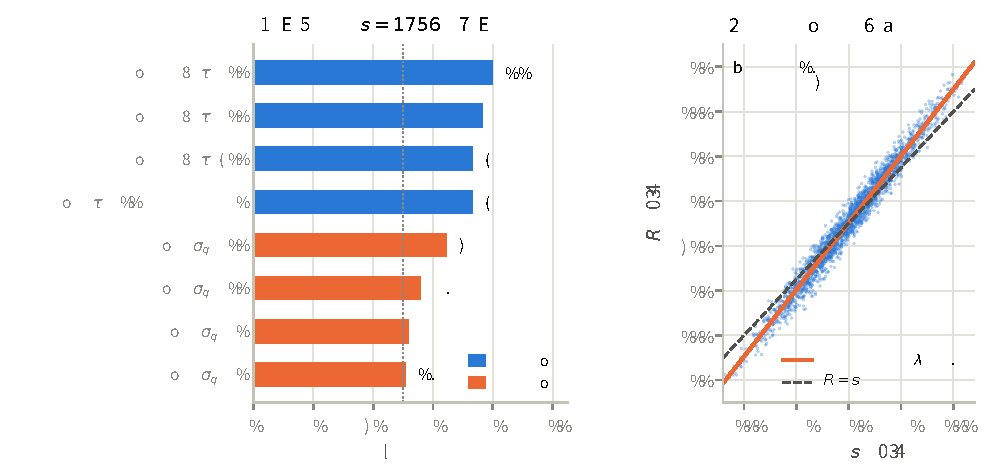
\includegraphics[width=\textwidth]{ch2/three_quantities.pdf}
  \caption{同一实力在不同环境下的长期胜率不同；评分只是实力的带噪声、带刻度的估计。(a) 实力 $s=1756$（$\tau=200$ 群体的第 90 百分位，取实力在 $\pm15$ 分内的玩家平均）在不同对手池和匹配规则下的胜率；(b) 按分匹配（$\sigma_q=100$）第 3000 轮的评分与实力（随机抽 2,500 人作图）。参数：10,000 人，$s\sim\Normal(1500,\tau^2)$，$K=16$，3000 轮，统计第 1001–3000 局。\tagOwn}
  \label{fig:ch2-three}
\end{figure}

\subsection{评分是带噪声、带滞后、带刻度的估计}

TrueSkill~2 的定义很清楚：评分是“根据以往对局结果，对玩家赢下一局能力的估计”，论文还特意区分“玩家的实际实力”和“系统给出的评分”\cite{minka2018trueskill}\tagLit。把评分写成
\begin{equation}
  R_{i,t}=a+\lambda\,s_{i,t}+e_{i,t},
  \label{eq:ch2-rating}
\end{equation}
它与实力之间隔着四样东西：噪声 $e$（标准差 $\sigma_e\approx9.3\sqrt K$，\cref{sec:ch2-sbmm-error}）、滞后（误差衰减需要几十局）、刻度 $\lambda$ 与截距 $a$（零和评分池的整体漂移，以及按分匹配下的刻度伸缩，\cref{sec:ch2-stretch}）。\cref{fig:ch2-three}(b) 是按分匹配稳态下的评分：与实力的相关系数 0.986，排序几乎正确，但斜率 $\lambda=1.19$、残差 41 分\tagOwn。

\begin{keybox}[为什么胜率和分数都只体现一部分实力]
\begin{itemize}
\item \textbf{胜率}衡量的是实力相对“实际对手”的位置。随机匹配下它随实力单调变化，但同时取决于群体离散度和游戏随机性；按分匹配会让对手随你的评分一起移动，胜率便趋于 50\%，几乎不再反映实力（\cref{sec:ch2-sbmm}）。
\item \textbf{评分 / 段位分}衡量的是系统对实力的估计：有 $\pm\sigma_e$ 的噪声、几十局的滞后、随群体漂移的截距，在按分匹配下还可能有被拉伸的刻度；可靠的通常只有排序。可见段位往往还叠加了保底和加分（\cref{sec:ch2-rank}）。
\item \textbf{局内数据}（击杀、伤害、名次分）是另一种局部观测；TrueSkill~2 就把击杀数等作为额外证据\cite{minka2018trueskill}\tagLit，但它们与胜负的关系依赖位置和打法。
\item 可操作的定义：\textbf{实力是能预测“对任意对手胜率”的那个 $s$}。一个可观测的替代量是“对固定参照池的胜率”，在正态群体中它与实力百分位一一对应（\cref{eq:ch2-percentile}）。在按分匹配的数据里，应当从评分和对手评分反推实力，而不是看胜率。
\end{itemize}
\end{keybox}

% ======================================================================
\section{“每局五五开”是预测胜率相等，不是实力相等}
\label{sec:ch2-fair}

\subsection{匹配器拉平的是估计实力，等价于预测胜率 50\%}

匹配器看得到的只有评分。由于 $E=F(R_A-R_B)$ 是评分差的严格单调函数，“双方评分相等”与“系统预测胜率为 50\%”是同一件事；团队游戏里，“两队评分之和（或均值）相等”等价于“团队预测胜率为 50\%”。TrueSkill 用“平局概率”定义匹配质量，并指出“对局质量由结果的不可预测性决定”\cite{herbrich2006trueskill}\tagLit。暴雪说明《守望先锋 2》组局时只看当前 MMR，并称匹配器不会强制任何人 50\% 胜率\cite{blizzard2023overwatch}\tagOff；同一系列的第一篇把“公平对局”直接对应到 50\% 胜率\cite{blizzard2022overwatch}\tagOff。所以“五五开”是关于\emph{系统所掌握的信息}的陈述：在它知道的一切下，分不出谁更强。各厂商原话的逐条对照与“实力五五开、预测胜率五五开、长期胜率五五开”三种读法的辨析见\cref{sec:ch1b-fifty}；本节给出这一读法的数学后果。

\subsection{真实胜率围绕 50\% 分布，宽度由评分误差决定}

\textbf{假设}：评分处于稳态，$R=s+e$，$e\sim\Normal(0,\sigma_e^2)$ 与 $s$ 独立；匹配器把评分恰好相等的两人配成一局。\textbf{推导}：给定 $R$，实力的条件分布是正态，方差 $v=\tau^2\sigma_e^2/(\tau^2+\sigma_e^2)$，两人条件独立，均值相同，于是
\begin{equation}
  \begin{gathered}
  s_A-s_B\mid R_A=R_B\ \sim\ \Normal\!\Bigl(0,\ \frac{2\tau^2\sigma_e^2}{\tau^2+\sigma_e^2}\Bigr),\qquad
  p=F(s_A-s_B),\\
  f_p(x)=\frac{\phi\bigl(F^{-1}(x)/\sigma_\Delta\bigr)}{\sigma_\Delta\,c\,x(1-x)},
  \end{gathered}
  \label{eq:ch2-fair}
\end{equation}
其中 $\sigma_\Delta$ 是实力差的标准差（推导见\cref{app:ch2-fair}）。\textbf{数值}：$K=16$ 时 $\sigma_e=37.7$，$\sigma_\Delta=52.4$，90\% 的“五五开”对局真实胜率在 37.8\%–62.2\% 之间，$|p-\tfrac12|$ 平均 5.9 个百分点；$K=32$ 时 $\sigma_\Delta=73.7$，区间放宽到 33.2\%–66.8\%，平均偏离 8.2 个百分点\tagOwn。从模拟的稳态评分表中把评分相邻的两人配对，得到的区间是 38.3\%–62.1\% 和 33.7\%–66.0\%，平均偏离 5.8 和 8.1 个百分点（\cref{fig:ch2-fair}(a)）\tagOwn。

\begin{figure}[htbp]
  \centering
  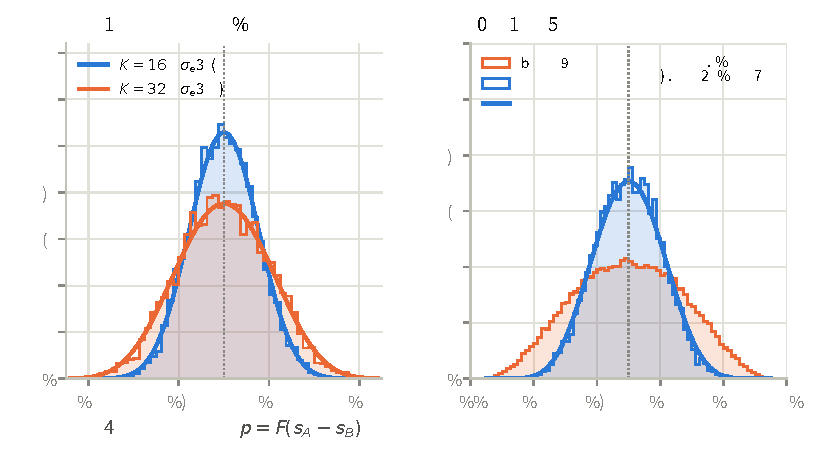
\includegraphics[width=\textwidth]{ch2/fair_game.pdf}
  \caption{“五五开”的一局，真实胜率并不是 50\%。(a) 1v1：把稳态评分表中评分相邻的两人配成一局，直方图为真实胜率 $p=F(s_A-s_B)$，曲线为\cref{eq:ch2-fair}；(b) 5v5（加和模型，$K=16$）：按 $R+\Normal(0,100^2)$ 排序每 10 人一局，在 126 种分队中选评分和最接近的一种，比较团队真实胜率与随机分配位置后的“对位单挑”真实胜率。评分表取自随机匹配模拟第 3000 轮（10,000 人，$\tau=200$）；(b) 重复组局 10 次，共 10,000 局。\tagOwn}
  \label{fig:ch2-fair}
\end{figure}

\subsection{团队游戏：总和相等，个人可以很悬殊}

团队匹配拉平的是两队评分的合计。加和模型下（\cref{sec:ch2-team}）团队实力差为 $(\sum s_A-\sum s_B)/\sqrt n$，给定两队评分和相等时它的方差同样是 $2v$，只是团队游戏中个人评分误差更大（$K=16$、5v5 时约 58 分，\cref{sec:ch2-team}），于是 90\% 的团队对局真实胜率落在 32\%–68\%（模拟 32.8\%–66.9\%）\tagOwn。个人层面更悬殊：以 $\sigma_q=100$ 组局时，一局内 10 人的评分标准差约 84 分，把双方队员随机两两“对位”，90\% 的单挑真实胜率落在 22\%–78\%，约 26\% 的对位偏离 50\% 超过 20 个百分点（\cref{fig:ch2-fair}(b)）\tagOwn。暴雪描述过同一现象：整局是平衡的，但一方高分坦克对上另一方低分坦克，这条对位会“非常一边倒”\cite{blizzard2022overwatch}\tagOff。

\subsection{这不是关于长期胜率的陈述}

“每局预测 50\%”和“长期胜率 50\%”是两件事。随机匹配下每局预测并不是 50\%，长期胜率也不是；按分匹配下两者都接近 50\%，但长期胜率趋于 50\% 的原因是\cref{sec:ch2-identity}的恒等式：实力优势被换成了更高的评分，而不是某种“拉回 50\%”的干预。反过来，真实匹配器也做不到每局恰好 50\%：排队时间要求放宽窗口，天梯两端人少，“没有同水平对手”时预测胜率就会偏离 50\%（\cref{sec:ch2-window}）。

% ======================================================================
\section{1v1 随机匹配：胜率由实力百分位和运气比例决定}
\label{sec:ch2-random}

\textbf{假设}：每局对手从全体中随机抽取，对手实力 $t\sim\Normal(\mu,\tau^2)$，胜率 $F(s-t)$。此时胜负与评分无关，$K$ 只影响评分，不影响胜率。

\begin{derivbox}[随机匹配的闭式胜率]
用 $F(d)\approx\Phi(d/\sigma_d)$，并利用恒等式 $\E\bigl[\Phi(a+bZ)\bigr]=\Phi\bigl(a/\sqrt{1+b^2}\bigr)$（$Z\sim\Normal(0,1)$；证明：$\Phi(a+bZ)=\Prob(Z'\le a+bZ\mid Z)$，而 $Z'-bZ\sim\Normal(0,1+b^2)$）：
\begin{equation}
  W(s)=\E_t\Bigl[\Phi\Bigl(\tfrac{s-t}{\sigma_d}\Bigr)\Bigr]=\Phi\Bigl(\frac{s-\mu}{\sqrt{\sigma_d^2+\tau^2}}\Bigr).
  \label{eq:ch2-random}
\end{equation}
写成实力百分位 $q$（$s=\mu+\tau z_q$）：
\begin{equation}
  W(q)=\Phi(r\,z_q),\qquad r=\frac{\tau}{\sqrt{\tau^2+\sigma_d^2}}.
  \label{eq:ch2-percentile}
\end{equation}
$r^2$ 是固定自身实力、对手随机时，“两人表现差”的方差中由对手实力离散解释的份额（两人都随机抽取时这一份额为 $2\tau^2/(2\tau^2+\sigma_d^2)$，$\tau=200$ 时 0.48）。单局另有独立噪声 $x\sim\Normal(0,\sigma_x^2)$ 时，把 $\sigma_d$ 换成 $\sigma_d'=\sqrt{\sigma_d^2+2\sigma_x^2}$。
\end{derivbox}

\Cref{tab:ch2-tau} 给出不同群体离散度下的数值。注意“前 10\% 平均”要对组内每个人的胜率求平均，不能把组内平均 $z$ 代入公式，后者因为 $\Phi$ 的凹性会偏高（$\tau=200$ 时 83.7\% 对 83.1\%）。

\begin{table}[htbp]
  \centering\small
  \caption{随机匹配 1v1 的长期胜率与群体实力离散度 $\tau$（$\sigma_d=295.7$）。百分位列用\cref{eq:ch2-percentile}；组平均列对组内每人的精确逻辑斯蒂胜率求平均。\tagOwn}
  \label{tab:ch2-tau}
  \begin{tabular}{rrrrrrr}
    \toprule
    $\tau$ & $r$ & $r^2$ & 第 75 百分位 & 第 90 百分位 & 前 10\% 平均 & 前 1\% 平均\\
    \midrule
    100 & 0.320 & 0.10 & 58.6\% & 65.9\% & 71.7\% & 80.7\%\\
    150 & 0.452 & 0.20 & 62.0\% & 71.9\% & 78.5\% & 88.2\%\\
    200 & 0.560 & 0.31 & 64.7\% & 76.4\% & 83.1\% & 92.5\%\\
    300 & 0.712 & 0.51 & 68.5\% & 81.9\% & 88.2\% & 96.4\%\\
    400 & 0.804 & 0.65 & 70.6\% & 84.9\% & 90.8\% & 97.9\%\\
    \bottomrule
  \end{tabular}
\end{table}

\textbf{模拟}：10,000 人、$\tau=200$、$K=16$，每人统计 2,000 局，十分位（按实力把玩家分成十等份）平均胜率依次为 17.0、27.9、35.0、41.2、47.1、52.9、58.8、65.1、72.1、82.9\%，精确积分值为 16.9…83.1\%，差别不超过 0.2 个百分点；前 1\% 为 92.7\%（公式 92.5\%），个人长期胜率的标准差为 19.6 个百分点\tagOwn。$K=32$ 的胜率与 $K=16$ 完全相同，因为同一随机种子下配对和胜负都与评分无关\tagOwn。

\textbf{两个敏感性}（\cref{fig:ch2-random}）：
\begin{itemize}
\item \textbf{群体离散度 $\tau$}：同一百分位，$\tau$ 越大（高手和新手差得越远）胜率越极端。TrueSkill 团队在 Xbox Live 上也观察到，运气型游戏（单局双陆棋、UNO）的实力分布窄，技巧型游戏（拟真赛车）的实力分布宽\cite{herbrich2006trueskill}\tagLit——用本节的话说，就是 $r$ 不同。群体整体变强（$\mu$ 上升）而你不变时，你的百分位下降，胜率也随之下降。
\item \textbf{单局随机性 $\sigma_x$}：$\sigma_x=150$ 时 $\sigma_d'=364$，两两胜率曲线（对实力差）的斜率变为原来的 0.81 倍，随机匹配下 $W(q)$ 曲线的斜率变为 $r'/r=357/415=0.86$ 倍，最强 10\% 从 82.9\% 降到 79.4\%（模拟）\tagOwn。Elo 会把预测胜率校准到观测胜率，所以评分差也按同一比例压缩：模拟中评分对实力的斜率为 0.811（理论 0.813）\tagOwn。评分度量的是“以胜率为单位的实力”。
\end{itemize}

\begin{figure}[htbp]
  \centering
  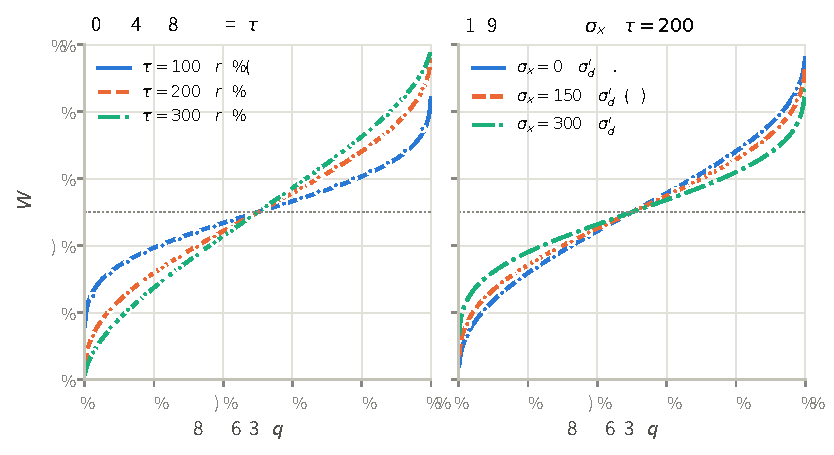
\includegraphics[width=\textwidth]{ch2/random_1v1.pdf}
  \caption{随机匹配 1v1 的长期胜率随实力百分位变化。曲线为\cref{eq:ch2-percentile}，点为模拟（每 5\% 百分位一组的平均胜率）。(a) 群体离散度 $\tau=100/200/300$；(b) 单局独立噪声 $\sigma_x=0/150/300$（$\tau=200$；$\sigma_x=300$ 只画公式）。参数：10,000 人，$K=16$，随机配对，3000 轮，统计第 1001–3000 局。\tagOwn}
  \label{fig:ch2-random}
\end{figure}

随机匹配下评分也能准确恢复实力：Aldous 证明随机配对的 Elo 过程有唯一平稳分布\cite{aldous2017elo}\tagLit，Cortez 与 Tossounian 进一步证明平稳分布以 $\sqrt K$ 的速度集中到真实实力\cite{cortez2024convergence}\tagLit，Olesker-Taylor 与 Zanetti 证明时间平均后的评分以高概率逼近真实参数\cite{oleskertaylor2024analysis}\tagLit。这些定理都假设“谁和谁对局”与当前评分无关；按分匹配不满足这一条件，Jabin 与 Junca 的连续模型显示，只与评分相近者对局时可能出现依赖初值的多个平衡态和很慢的收敛，评分却仍会收敛、看起来一切正常\cite{jabin2015continuous}\tagLit。这正是下一节要处理的情形。

% ======================================================================
\section{1v1 按分匹配：实力被兑换成评分}
\label{sec:ch2-sbmm}

\subsection{一条恒等式说明实力优势去了哪里}
\label{sec:ch2-identity}

固定 $K$ 的 Elo 每局评分变化为 $\Delta R_t=K(y_t-E_t)$。对 $T$ 局求和，$R_T-R_0=K\sum_t(y_t-E_t)$，两边除以 $KT$ 并移项：
\begin{equation}
  W_T\equiv\frac1T\sum_{t=1}^T y_t=\bar E_T+\frac{R_T-R_0}{K\,T}.
  \label{eq:ch2-identity}
\end{equation}
这是代数恒等式，对任何匹配方式都精确成立；在本章所有 1v1 和 5v5 模拟中，左右两边之差不超过 $4\times10^{-15}$\tagOwn。它说明长期胜率偏离 50\% 只有两个来源：一是匹配器系统性地给你更弱或更强的对手（$\bar E\ne\tfrac12$）；二是你的评分还在单向移动（新号、正在进步、刻度在伸缩）。严格按分匹配让 $\bar E\approx\tfrac12$，评分到达稳态后 $R_T-R_0$ 有界，于是 $W_T\to\tfrac12$，偏差按 $1/T$ 衰减：实力强 $\Rightarrow$ 评分高 $\Rightarrow$ 对手强 $\Rightarrow$ 单局胜率回到 50\%。

可变步长时（Glicko 的评分偏差、TrueSkill 的不确定度 $\sigma$\cite{herbrich2006trueskill}、新号阶段放大的 $K$），恒等式变成加权形式 $\sum_tK_t(y_t-E_t)=R_T-R_0$；连胜加分、段位保底等不经过 $K(y-E)$ 的改动会直接打破它。《守望先锋 2》对新号和回流玩家使用的“连胜调节”（胜率高于 50\% 时加快 MMR 上升）就是一种可变步长\cite{blizzard2022overwatch}\tagOff。

\subsection{评分的稳态误差约为 $9.3\sqrt K$，衰减需要 30–65 局}
\label{sec:ch2-sbmm-error}

\textbf{假设}：对手评分与自己相近，各自误差独立同分布。\textbf{推导}：令 $e=R-s$，线性化 $F(s-s')\approx\tfrac12+\tfrac c4(s-s')$，得 AR(1) 型递推
\begin{equation}
  e_{t+1}=\Bigl(1-\frac{Kc}4\Bigr)e_t+\frac{Kc}4e'_t+K\eta_t,\qquad \Var(\eta_t)\approx\tfrac14,
\end{equation}
平稳方差为
\begin{equation}
  \sigma_e^2=\frac{K}{2c\,(1-Kc/4)}\approx\frac{200K}{\ln10},\qquad \sigma_e\approx9.32\sqrt K,
  \label{eq:ch2-sigmae}
\end{equation}
误差的理想时间常数为 $4/(Kc)=1600/(K\ln10)\approx695/K$ 局（推导见\cref{app:ch2-linear}）。\Cref{tab:ch2-sigmae} 给出常用 $K$ 的数值。

\begin{table}[htbp]
  \centering\small
  \caption{Elo 评分误差的线性化数值（$\lambda=1$）。“修正”列含对手误差项；半衰期按离散递推 $-\ln2/\ln(1-Kc/4)$ 计算；“实测”为模拟中误差自相关降到 $1/e$ 的局数。\tagOwn}
  \label{tab:ch2-sigmae}
  \setlength{\tabcolsep}{4.5pt}
  \begin{tabular}{rrrrrc}
    \toprule
    $K$ & $\sqrt{200K/\ln10}$ & $\sigma_e$（修正） & 理想时间常数 $4/(Kc)$ & 半衰期 & 实测衰减时间\\
    &&&&& （按分 $\sigma_q$=100 / 200 / 随机）\\
    \midrule
    10 & 29.5 & 29.7 & 69.5 & 47.8 & —\\
    16 & 37.3 & 37.7 & 43.4 & 29.8 & 55 / 59 / 66\\
    20 & 41.7 & 42.3 & 34.7 & 23.7 & —\\
    32 & 52.7 & 54.0 & 21.7 & 14.7 & 34 / 30 / 34\\
    40 & 58.9 & 60.7 & 17.4 & 11.7 & —\\
    \bottomrule
  \end{tabular}
\end{table}

模拟证实了 $\sqrt K$ 规律：随机匹配下 $K=8,16,24,32,48,64$ 的残差标准差为 26.5、37.8、46.7、54.5、67.9、79.9，公式为 26.5、37.7、46.5、54.0、66.9、78.2（\cref{fig:ch2-error}(a)）\tagOwn。按分匹配下误差略大，因为刻度 $\lambda>1$ 时 $\sigma_e^2$ 按 $\lambda$ 放大（\cref{app:ch2-linear}）。

但 695/K 只是下限。它要求 $\lambda=1$ 且每局 $P(1-P)=\tfrac14$，这两条从不同时成立：随机匹配下对手常常差得远，$P(1-P)<\tfrac14$；按分匹配下配到的对手评分会向均值回归，而且 $\lambda>1$ 会削弱回复力。把这两项写进系数 $\kappa_R=4\E[P(1-P)]\cdot(\lambda\tau^2+\sigma_q^2)/(\sigma_R^2+\sigma_q^2)$（只在本节使用，与第三章的 $\kappa$ 不同），时间常数为 $4/(Kc\kappa_R)$：$K=16$ 时按分匹配为 56–58 局，随机匹配（各人恢复速度不同的混合）为 65 局，实测为 55、59、66 局；$K=32$ 时公式 30–34 局，实测 30–34 局（\cref{fig:ch2-error}(b)）\tagOwn。所以现实的匹配条件下，$K=16$ 的评分误差约 55–65 局才衰减到 $1/e$，$K=32$ 约 30–34 局。这与 Aldous 的看法一致：Elo 在“滞后”和“噪声”之间取舍，$K$ 小则噪声小、滞后大\cite{aldous2017elo}\tagLit。

\begin{figure}[htbp]
  \centering
  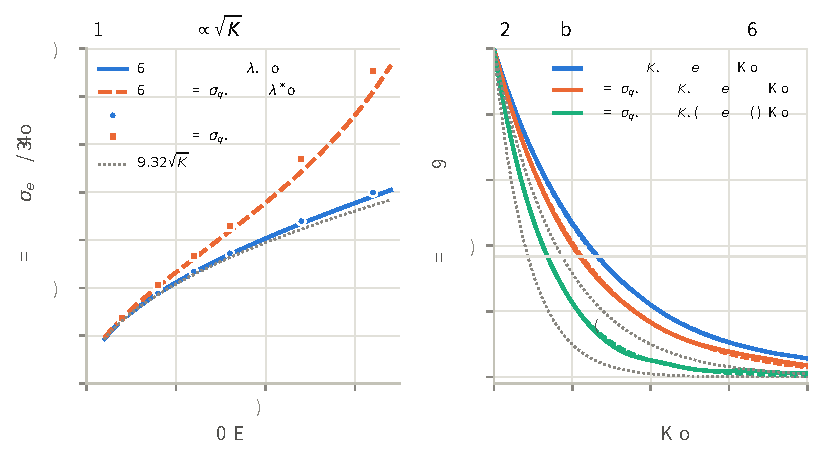
\includegraphics[width=\textwidth]{ch2/rating_error.pdf}
  \caption{评分误差的大小与衰减。(a) 稳态误差（相对评分–实力回归线的残差标准差）随 $K$ 的变化，曲线为\cref{eq:ch2-sigmae}（按分匹配取平稳刻度 $\lambda^*$），点为模拟（4,000 人，2,500 轮，预热 1,000 轮后每 50 轮取一次残差并平均）；(b) 评分误差的自相关：实线为模拟（10,000 人中前 2,000 人第 1001–1400 轮的逐轮评分），虚线为修正后的时间常数，灰色点线为理想值 $695/K$。\tagOwn}
  \label{fig:ch2-error}
\end{figure}

\subsection{匹配窗口决定天梯两端偏离 50\% 多少}
\label{sec:ch2-window}

真实匹配器在一个窗口内找对手。我们用“按 $R+\xi$ 排序后相邻配对，$\xi\sim\Normal(0,\sigma_q^2)$”来模拟，$\sigma_q$ 越大窗口越宽。配到的两人评分差的标准差约为 $\sqrt{2g}\,\sigma_q$（$g$ 见下式）：$\sigma_q=20$ 时约 28 分，系统预测胜率 90\% 落在 43\%–57\%；$\sigma_q=100$ 时约 132 分，预测胜率 90\% 落在 23\%–78\%，已是相当宽松的匹配\tagOwn。

\textbf{推导}（\cref{app:ch2-edge}）：设评分在群体中的标准差为 $\sigma_R$，排序键 $k=R+\xi$，相邻者的键几乎相同。给定自己的评分 $R$，对手评分 $R'$ 服从
\begin{equation}
  \begin{gathered}
  R-R'\sim\Normal\bigl((1-g)(R-\mu),\ g(1+g)\sigma_q^2\bigr),\qquad g=\frac{\sigma_R^2}{\sigma_R^2+\sigma_q^2},\\
  W\approx\bar E\approx\Phi\Biggl(\frac{(1-g)(R-\mu)}{\sqrt{\sigma_d^2+g(1+g)\sigma_q^2}}\Biggr).
  \end{gathered}
  \label{eq:ch2-edge}
\end{equation}
高分玩家平均遇到评分更低的对手，低分玩家相反。这不是操纵，而是“窗口对称、人口密度不对称”的结果，天梯顶端尤其明显；暴雪也提到最高分段“玩家少得多”，组局时更难避免分差\cite{blizzard2022overwatch}\tagOff。

\textbf{数值}（\cref{fig:ch2-sbmm}）：$K=16$ 时最弱到最强十分位的胜率为：随机匹配 17.0\%–82.9\%，$\sigma_q=200$ 时 30.9\%–69.1\%，$\sigma_q=100$ 时 42.1\%–58.0\%，$\sigma_q=50$ 时 47.6\%–52.4\%，$\sigma_q=20$ 时 48.8\%–51.2\%\tagOwn。$K=32$ 的对应值为 31.6\%–68.4\%、43.5\%–56.5\%、48.3\%–51.7\%、48.9\%–51.1\%\tagOwn。\Cref{eq:ch2-edge} 给出的最强十分位胜率为 57.8\%（$K=16$，$\sigma_q=100$，模拟 58.0\%）、69.3\%（$\sigma_q=200$，模拟 69.1\%）、56.7\%（$K=32$，$\sigma_q=100$，模拟 56.5\%）\tagOwn。

用\cref{eq:ch2-identity}分解：$\sigma_q=100$ 时偏离 50\% 的部分几乎全在 $\bar E$ 一项，评分项只有 $\pm0.05$ 个百分点；$\sigma_q=20$ 时 $\bar E$ 只在 49.7\%–50.3\%，剩下的 $\pm0.9$ 个百分点来自评分项，即下文的刻度拉伸，它随时间减小\tagOwn。

\begin{figure}[htbp]
  \centering
  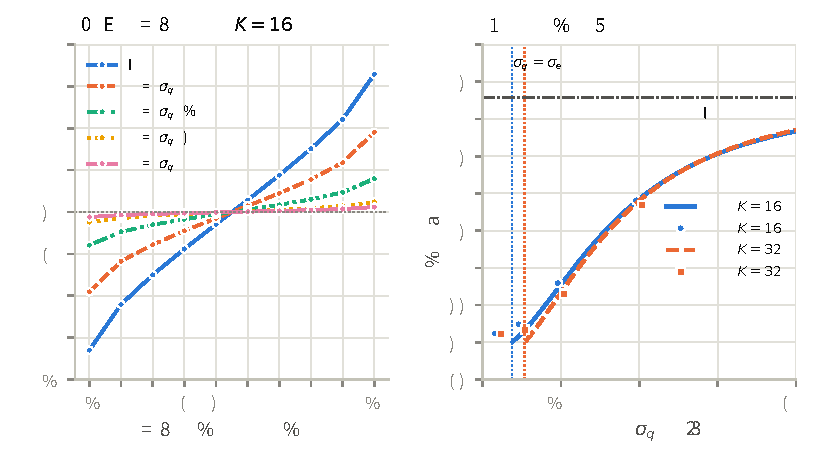
\includegraphics[width=\textwidth]{ch2/sbmm_deciles.pdf}
  \caption{按分匹配把各实力十分位的胜率压向 50\%，压到什么程度由匹配窗口决定。(a) $K=16$ 时各十分位的长期胜率；(b) 最强 10\% 的胜率随匹配噪声 $\sigma_q$ 的变化，曲线为\cref{eq:ch2-edge}（只在 $\sigma_q>\sigma_e$、存在平稳刻度时画出），点为模拟（左右略错开以免重叠），点线标出 $\sigma_q=\sigma_e$。参数：10,000 人，$\tau=200$，按 $R+\Normal(0,\sigma_q^2)$ 排序相邻配对，3000 轮，统计第 1001–3000 局。\tagOwn}
  \label{fig:ch2-sbmm}
\end{figure}

\subsection{新号与回流：强玩家从 1500 起步要几十局才能追回}
\label{sec:ch2-reset}

系统平稳后，从实力前 10\% 中抽 500 人，把评分重置为 1500（相当于高手开新号），跟踪其后 400 局。差距用“实力 $-$ 评分折算的实力”计量，折算用的回归线每轮在未重置玩家上重新拟合。结果（\cref{fig:ch2-reset}）：初始差距约 350 实力分；按分匹配下追回一半需要 47 局（$K=16$）或 30 局（$K=32$），追回 90\% 需要 150 局或 96 局；随机匹配下为 50/191 局和 26/101 局\tagOwn。按分匹配的前 50 局胜率为 77.5\%（$K=16$）和 73.6\%（$K=32$），前 100 局为 72.9\% 和 68.0\%，第 301–400 局回落到 58.9\% 和 57.1\%，即前 10\% 玩家在该窗口下的平稳胜率；随机匹配下胜率与评分无关，始终约 83\%\tagOwn。

两点说明。第一，若把目标线固定在重置前一刻，追回 90\% 看起来要 304 局（$K=16$）和 257 局（$K=32$）：在零和评分池里，把 500 人的评分从约 1920 拉到 1500 会让整个评分池下沉约 20 分，固定目标忽略了这一点\tagOwn。第二，大差距时单局胜率接近饱和，每局最多涨 $K/2$，所以前期比线性理论慢。TrueSkill 在 Xbox Live 上观察到，新玩家若前几局持续输球，整体实力分布会落到先验以下；一次实力重置之后，在更严格的匹配下这一现象消失\cite{herbrich2006trueskill}\tagLit；《守望先锋 2》则通过降低新号初始 MMR 并加快初期调整来处理新玩家胜率偏低的问题\cite{blizzard2022overwatch}\tagOff。

\begin{figure}[htbp]
  \centering
  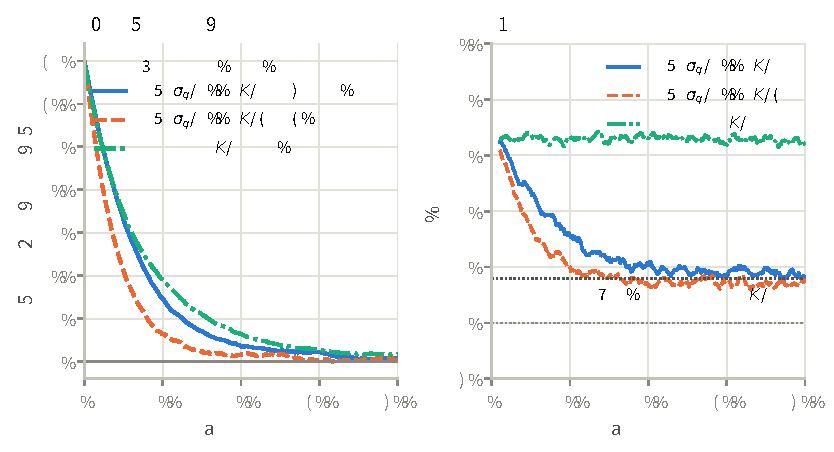
\includegraphics[width=\textwidth]{ch2/reset.pdf}
  \caption{强玩家评分被重置为 1500 后的追分过程。(a) 评分落后于实力的程度（实力分），括号内为追回 50\% / 90\% 差距所需局数；(b) 这批玩家的胜率（10 局滑动平均），点线为按分匹配平稳时前 10\% 玩家的胜率。参数：10,000 人，$\tau=200$，系统运行 1000 轮后从实力前 10\% 中随机重置 500 人，按分匹配 $\sigma_q=100$ 或随机匹配，$K=16/32$。\tagOwn}
  \label{fig:ch2-reset}
\end{figure}

\subsection{严格按分匹配会拉伸评分刻度（理想模型的性质）}
\label{sec:ch2-stretch}

这一节讨论的是本项目在理想模型中推导并模拟出来的性质，\textbf{没有在真实数据中观测到}。

\textbf{精确的出发点}：两名评分完全相等的玩家对局，$E=\tfrac12$，无论谁赢，两人评分都变成 $R\pm K/2$。于是每局使群体评分方差恰好增加 $K^2/4$。只要配对时对手的实力与自己“在给定评分下可交换”，就有 $\Cov(R,\,y-E)=0$，没有任何力量把这部分方差收回。模拟中以 $\sigma_q=0$ 确定性配对 3000 局，评分方差增加 191,792，理论值 $16^2\times3000/4=192{,}000$\tagOwn。方差增加而排序不变，表现为评分对实力的斜率 $\lambda$ 增大，上包络（配对评分完全相等时的理论上限）为 $\lambda(t)^2\approx\lambda_0^2+K^2t/(4\tau^2)$。

\textbf{一般窗口}（\cref{app:ch2-stretch}）：用\cref{eq:ch2-rating}的线性结构做平均场近似（把每名玩家受到的匹配影响换成群体平均），
\begin{equation}
  \frac{\dd\lambda}{\dd t}=\frac{Kc}{4}\cdot\frac{\sigma_e^2+\sigma_q^2(1-\lambda)}{\lambda^2\tau^2+\sigma_e^2+\sigma_q^2},\qquad
  \lambda^*=\frac{1}{1-\sigma_e^2/\sigma_q^2}.
  \label{eq:ch2-stretch}
\end{equation}
分子第一项是“同分对局把评分拉开”，第二项是“窗口内遇到不同评分的对手把刻度拉回”。平稳刻度只在 $\sigma_q>\sigma_e$ 时存在，即配对评分差的标准差要大于约 $\sqrt2\sigma_e$（$K=16$ 时约 53 分，$K=32$ 时约 76 分）。$K=16$ 时 $\lambda^*$ 在 $\sigma_q=50,100,200$ 下为 2.32、1.17、1.04；$K=32$ 时 $\sigma_q=100,200$ 下为 1.41、1.08\tagOwn。模拟（初始评分等于实力，$\lambda_0=1$）第 10,000 局的斜率为：$\sigma_q=20$ 时 3.75（方程 3.77，上包络 4.12），$\sigma_q=50$ 时 2.16 并仍在上升（方程 2.11），$\sigma_q=100$ 时 1.20（1.17），$\sigma_q=200$ 时 1.06（1.04）（\cref{fig:ch2-stretch}）\tagOwn。

\textbf{含义}：刻度被拉伸时排序依然准确（相关系数 0.99），但评分差夸大了实力差，用评分差预测的胜率会过于自信；本章 $\sigma_q=20$ 下各十分位的残余偏离（$\pm0.9$ 个百分点）就是 $\lambda$ 仍在增长带来的评分项。部署中的系统有很多这一模型没有的“锚”：新玩家以默认分进入、赛季软重置、长期不玩后的调整\cite{blizzard2022overwatch}\tagOff、段位保底\cite{blizzard2020developer}\tagOff、排队时间带来的窗口放宽，它们都可能限制拉伸。我们的判断是：无界的 $\sqrt t$ 增长在真实系统中不太可能出现，有界的轻度放大（$\lambda^*$ 在 1.05–1.5 之间）是可能的，但未见实证。

\begin{figure}[htbp]
  \centering
  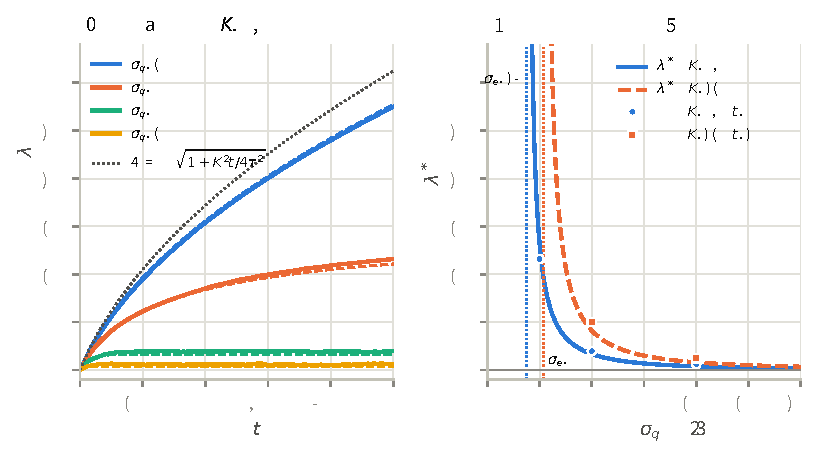
\includegraphics[width=\textwidth]{ch2/stretch.pdf}
  \caption{严格按分匹配下评分刻度的拉伸（理想模型的性质，不是真实数据中的观测）。(a) 评分对实力的回归斜率 $\lambda(t)$：实线为模拟，同色虚线为\cref{eq:ch2-stretch}的平均场方程，灰色点线为配对评分完全相等时的上包络；(b) 平稳斜率 $\lambda^*$ 与匹配噪声 $\sigma_q$，点线为 $\sigma_q=\sigma_e$。参数：(a) 2,000 人，$\tau=200$，$K=16$，初始评分 $=$ 实力，10,000 轮；(b) 圆点取自 (a) 第 10,000 轮，方块取自 10,000 人、初始评分全为 1500、$K=32$ 的模拟第 3,000 轮。\tagOwn}
  \label{fig:ch2-stretch}
\end{figure}

\subsection{可见段位与隐藏分}
\label{sec:ch2-rank}

主流做法是用隐藏分（MMR）匹配，用可见段位提供进度感。暴雪说明《守望先锋 2》组局“从不使用”玩家看到的段位，只看 MMR\cite{blizzard2022overwatch}\tagOff。《炉石传说》酒馆战棋 2020 年起也采用“双评分”：匹配只用内部评分，外显评分叠加保底和进度分\cite{blizzard2020developer}\tagOff（各厂商的做法见\cref{sec:ch1b-blizzard}与\cref{tab:ch1b-disclosure}）。对本章的公式而言，这意味着：
\begin{itemize}
\item 匹配时“段位或分数”影响胜率，只是通过隐藏分决定对手分布 $\mathcal G$；\cref{eq:ch2-identity}适用于隐藏分（若其步长固定）。
\item 可见段位叠加了保底和加分，它的变化不再满足 $K(y-E)$，赛季内会系统性上漂，不宜直接用来估计实力或胜率。
\item 同段位的两个人可能隐藏分相差很大，所以“我和对面段位一样却被碾压”并不与“预测胜率 50\%”矛盾。
\end{itemize}

% ======================================================================
\section{每局人数：团队稀释个人优势，多人局改变基准}
\label{sec:ch2-players}

\subsection{团队游戏：加和模型约按 $1/\sqrt n$ 稀释，均值模型约按 $1/n$}
\label{sec:ch2-team}

\textbf{假设}：焦点玩家比群体平均高 $d$ 分，$n-1$ 名队友和 $n$ 名对手都从 $\Normal(\mu,\tau^2)$ 随机抽取。两种团队模型：
\begin{itemize}
\item \textbf{加和模型}：每名队员有独立表现噪声，团队表现为队员表现之和（TrueSkill 的假设\cite{herbrich2006trueskill}\tagLit），用逻辑斯蒂类比写成 $P=F\bigl((\sum s_A-\sum s_B)/\sqrt n\bigr)$；
\item \textbf{均值模型}：随机性主要在团队层面（地图、阵容、配合），$P=F(\bar s_A-\bar s_B)$。
\end{itemize}
\textbf{推导}：加和模型下自变量 $X=(d+\sum_{n-1}t_i-\sum_n o_j)/\sqrt n\sim\Normal\bigl(d/\sqrt n,\ (2n-1)\tau^2/n\bigr)$，均值模型下 $X\sim\Normal\bigl(d/n,\ (2n-1)\tau^2/n^2\bigr)$，再用\cref{eq:ch2-random}的高斯恒等式：
\begin{equation}
  W_{\text{加和}}\approx\Phi\Biggl(\frac{d/\sqrt n}{\sqrt{\sigma_d^2+(2n-1)\tau^2/n}}\Biggr),\qquad
  W_{\text{均值}}\approx\Phi\Biggl(\frac{d/n}{\sqrt{\sigma_d^2+(2n-1)\tau^2/n^2}}\Biggr).
  \label{eq:ch2-team}
\end{equation}
稀释有两层：个人优势在团队差中只占 $1/\sqrt n$ 或 $1/n$；队友和对手的实力离散 $(2n-1)\tau^2$ 又加了一层噪声。$n$ 较大时，加和模型在 $d=0$ 处的斜率约为 $\phi(0)/\bigl(\sqrt n\sqrt{\sigma_d^2+2\tau^2}\bigr)\propto1/\sqrt n$，均值模型约为 $\phi(0)/(n\sigma_d)\propto1/n$。$n=5$ 时斜率分别是 1v1 的 0.40 和 0.23 倍（$1/\sqrt5=0.45$，$1/5=0.20$）\tagOwn。

\begin{table}[htbp]
  \centering\small
  \caption{随机队友、随机对手时团队人数对个人胜率的稀释（$\tau=200$，精确数值积分）。提升量按 $d=0$ 附近的斜率计算；末列为队友与对手都和群体平均同水平时的加和模型。\tagOwn}
  \label{tab:ch2-team}
  \setlength{\tabcolsep}{5pt}
  \begin{tabular}{rrrrrr}
    \toprule
    & \multicolumn{2}{c}{最强 10\% 的胜率} & \multicolumn{3}{c}{每 100 分优势的胜率提升（百分点）}\\
    \cmidrule(lr){2-3}\cmidrule(lr){4-6}
    $n$ & 加和 & 均值 & 加和 & 均值 & 加和，同水平队友\\
    \midrule
    1 & 83.1\% & 83.1\% & 11.4 & 11.4 & 14.4\\
    2 & 73.9\% & 69.7\% & 7.4 & 6.0 & 10.2\\
    3 & 69.6\% & 64.1\% & 5.9 & 4.1 & 8.3\\
    5 & 65.2\% & 59.0\% & 4.5 & 2.6 & 6.4\\
    6 & 63.9\% & 57.6\% & 4.1 & 2.2 & 5.9\\
    8 & 62.1\% & 55.9\% & 3.5 & 1.7 & 5.1\\
    \bottomrule
  \end{tabular}
\end{table}

\textbf{模拟}（\cref{fig:ch2-team}）：随机分队的 5v5，加和模型十分位胜率为 34.8\%–65.2\%，前 1\% 为 72.8\%，个人长期胜率的标准差 8.8 个百分点（1v1 为 19.6）；均值模型为 41.0\%–59.0\%\tagOwn。哪种模型更接近真实取决于随机性在哪里：TrueSkill 在 Halo 2 的 4v4 夺旗模式中没能胜过 Elo，作者认为可能是因为加和假设不成立\cite{herbrich2006trueskill}\tagLit；TrueSkill~2 发现组队玩家的胜率高于“队员实力之和”所预测的值，于是加入组队偏移\cite{minka2018trueskill}\tagLit。

\begin{figure}[htbp]
  \centering
  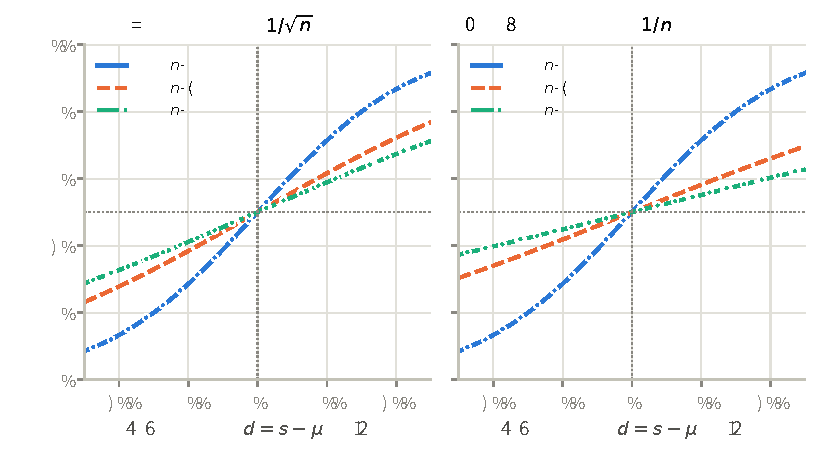
\includegraphics[width=\textwidth]{ch2/team.pdf}
  \caption{团队游戏稀释个人实力优势。焦点玩家比群体平均高 $d$ 分，队友和对手随机。曲线为\cref{eq:ch2-team}对应的精确数值积分；蓝点为 1v1 随机匹配模拟，绿点为 5v5 随机分队模拟（按实力每 50 分一组的平均胜率）。参数：$\tau=200$，10,000 人，$K=16$，3000 轮，统计第 1001–3000 局。\tagOwn}
  \label{fig:ch2-team}
\end{figure}

\textbf{团队的按分匹配}：按 $R+\Normal(0,\sigma_q^2)$ 排序每 10 人一组，组内按评分蛇形分队（从高到低按 ABBAABBAAB 交替选人，使两队评分尽量平衡），$\sigma_q=100$ 时加和模型十分位胜率为 48.7\%–51.3\%，均值模型 48.9\%–51.1\%，$\sigma_q=200$ 时加和模型为 48.1\%–52.0\%；但评分刻度在统计期内一直在拉伸（加和模型 $\sigma_q=100$ 时 $\lambda$ 从第 1000 局的 1.22 升到第 3000 局的 2.04，$\sigma_q=200$ 时从 1.20 升到 1.82），所以这些数字只是某一时刻的快照\tagOwn。分队按评分平衡后，个人实力几乎完全被换成评分；若分队与评分无关（随机分队），十分位胜率要宽得多（\cref{fig:ch2-team}）。团队中个人的评分误差也更大（随机分队）：加和模型的残差为 57.7 分（$K=16$），粗略公式 $\sqrt{K\sqrt n/\bigl(2c(1-\sqrt nKc/4)\bigr)}$ 给出 57.2；均值模型为 84.4 分；1v1 为 37.8 分\tagOwn。

\subsection{多人自由混战：Plackett–Luce 给出名次概率}
\label{sec:ch2-ffa}

\textbf{假设}：$N$ 人一局，表现为实力加 Gumbel 噪声（尺度 $400/\ln10$）。这一设定下，任意两人的相对名次概率恰为 Elo 的 $F$，而完整名次服从 Plackett–Luce 模型：权重（worth）$w_i=10^{s_i/400}$，从剩余玩家中按 $w$ 的比例依次抽出第一名、第二名……\cite{weng2011bayesian}\tagLit（推导见\cref{app:ch2-team}）。\textbf{推导}：焦点玩家对其余 $N-1$ 名同水平对手的优势为 $d$，$w=10^{d/400}$，
\begin{equation}
  \Prob(\text{第 1})=\frac{w}{w+N-1},\qquad
  \Prob(\text{前 }k)=1-\prod_{j=0}^{k-1}\frac{N-1-j}{w+N-1-j}.
  \label{eq:ch2-pl}
\end{equation}
后一式是“前 $k$ 次抽取都没有抽中焦点玩家”的补概率。

\begin{table}[htbp]
  \centering\small
  \caption{8 人自由混战（Plackett–Luce）中，对其余 7 名同水平对手的实力优势 $d$ 与名次指标。\tagOwn}
  \label{tab:ch2-ffa}
  \begin{tabular}{rrrrrr}
    \toprule
    $d$ & $w$ & 1v1 胜率 & 第 1 名 & 前 4 名 & 平均名次\\
    \midrule
    $-200$ & 0.32 & 24.0\% & 4.3\% & 20.8\% & 6.32\\
    0 & 1.00 & 50.0\% & 12.5\% & 50.0\% & 4.50\\
    $+100$ & 1.78 & 64.0\% & 20.3\% & 68.6\% & 3.52\\
    $+200$ & 3.16 & 76.0\% & 31.1\% & 84.6\% & 2.68\\
    $+400$ & 10.0 & 90.9\% & 58.8\% & 98.5\% & 1.64\\
    \bottomrule
  \end{tabular}
\end{table}

\begin{figure}[htbp]
  \centering
  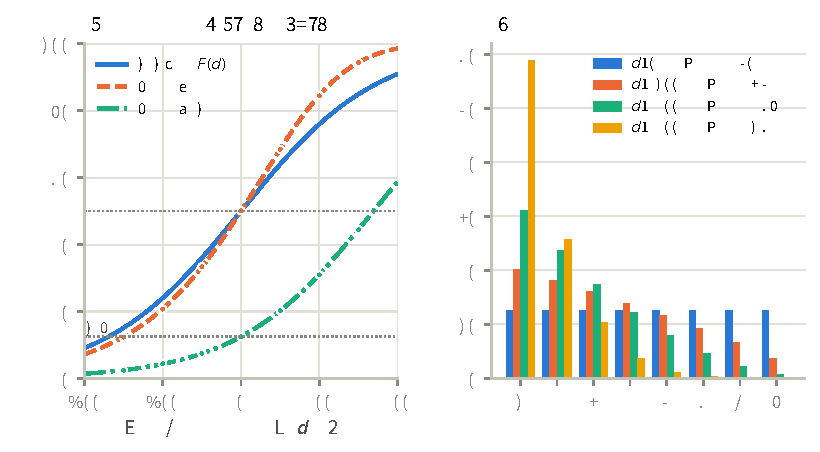
\includegraphics[width=\textwidth]{ch2/ffa.pdf}
  \caption{8 人自由混战中实力优势如何换成名次。(a) 对其余 7 名同水平对手的优势为 $d$ 时进前 4 名和拿第 1 名的概率（曲线为\cref{eq:ch2-pl}，点为 Gumbel 表现的蒙特卡洛，每点 20 万局），蓝线为 1v1 胜率作对照；(b) $d=0/{+}100/{+}200/{+}400$ 时的名次分布。\tagOwn}
  \label{fig:ch2-ffa}
\end{figure}

\textbf{“胜”的定义决定基准率}。按分匹配把同一局 8 人的估计实力拉平，于是均衡时第一名率趋于 $1/N=12.5\%$，前四率趋于 50\%，平均名次趋于 $(N+1)/2=4.5$。模拟（10,000 人，$K=16$，两两 Elo 更新每对步长 $K/7$）：随机组局时最强 10\% 的第一名率 39.8\%、前四率 93.1\%、平均名次 2.20，最弱 10\% 为 1.4\%、10.7\%、6.81；按分匹配（$\sigma_q=100$）时最强 10\% 为 17.0\%、61.3\%、3.90，最弱 10\% 为 8.9\%、39.2\%、5.10\tagOwn。对酒馆战棋这类“前四加分”的游戏，按分匹配下前四率约 50\% 并不说明水平一般；按“第一名”统计，基准是 12.5\%。

\textbf{多人局的评分误差更小}。每局给出 $N-1$ 组两两比较，每组步长 $K/(N-1)$。同水平时名次均匀，单局评分变化的方差为 $K^2(N+1)/\bigl(12(N-1)\bigr)$，而 1v1 为 $K^2/4$；回复力相同，于是 $\sigma_{e,\text{FFA}}=\sigma_e\sqrt{(N+1)/(3(N-1))}$，$N=8$、$K=16$ 时为 24.7 分，模拟为 24.7（按分匹配）和 22.6（随机组局），1v1 为 37.8\tagOwn。酒馆战棋的评分更新同样基于 8 人两两之间的 56 个预测胜率\cite{blizzard2019developer}\tagOff（\cref{sec:ch1b-blizzard}），但具体公式没有公开，本节的两两 Elo 只是常见近似。

% ======================================================================
\section{实力有波动时，期望胜率仍可计算，误差更大}
\label{sec:ch2-fluct}

把当局实力写成 $s_{i,t}=s_i+u_t$。三种波动的后果不同。本节只讨论胜率的水平与方差；“上头”这类由输赢反过来影响状态的反馈，以及它如何制造连败，见\cref{ch:streaks}。

\subsection{独立的单局波动：曲线变平，评分刻度同比例压缩}

$u_t$ 每局独立、标准差 $\sigma_x$ 时，$P=\E\,F(\Delta s+x_i-x_j)\approx\Phi\bigl(\Delta s/\sqrt{\sigma_d^2+2\sigma_x^2}\bigr)$，相当于游戏更随机（\cref{sec:ch2-random}）。Elo 把评分校准到“以胜率为单位的实力”，评分差压缩为实力差的 $\sigma_d/\sigma_d'$ 倍：$\sigma_x=150$ 时理论 0.813，模拟 0.811；随机匹配下十分位胜率 20.6\%–79.4\%，按分匹配（$\sigma_q=100$）下 40.9\%–59.1\%\tagOwn。

\subsection{自相关的状态：评分只吸收一部分，窗口胜率成段波动}
\label{sec:ch2-ar1}

\textbf{假设}：状态服从 AR(1)，$u_{t+1}=\rho u_t+\sqrt{1-\rho^2}\,\sigma_u\varepsilon_t$；取 $\sigma_u=100$，$\rho=0.99$（相关时间约 100 局），作为“状态好坏、疲劳、时段”的示意。

\textbf{评分是指数平滑器}。在实力单位下，Elo 每局把评分朝当局实力移动一个比例 $b=1/\tau_R$（与第三章的 $b$ 同义），即 $\hat s_{t+1}=(1-b)\hat s_t+b(s+u_t)+\text{噪声}$。决定第 $t$ 局胜率的是赛前评分 $\hat s_t$，它对当前状态的回归系数（“被吸收的份额”）为
\begin{equation}
  a=\frac{\Cov(\hat s_t,u_t)}{\sigma_u^2}=\frac{b\rho}{1-(1-b)\rho}.
  \label{eq:ch2-absorb}
\end{equation}
用理想值 $b=Kc/4$ 得 $a=0.70$（$K=16$）和 0.82（$K=32$）；用修正后的时间常数（$\sigma_q=100$ 时 56 局和 34 局）得 0.64 和 0.74，模拟为 0.63 和 0.73\tagOwn。没被吸收的 $(1-a)u_t$ 直接进入单局胜率，所以即使在按分匹配下，“手热”（$u>\sigma_u$）时也多赢：模拟胜率 58.9\%，“手冷”（$u<-\sigma_u$）时 41.1\%；近似公式 $F\bigl((1-a)\E[u\mid u>\sigma_u]\bigr)\approx F(0.36\times152)\approx57.8\%$\tagOwn。

\textbf{逐局几乎看不出，窗口胜率却明显更分散}。按分匹配下逐局结果的自相关只有 0.016（滞后 1 局）、0.014（5 局）、0.008（20 局），很难从单局层面察觉；但 $n$ 局窗口胜率的方差明显偏离二项分布。由\cref{eq:ch2-identity}，窗口胜率的波动来自 $\bar E$ 的局间波动和窗口内评分的净变化，后者的方差由评分对 $s+u$ 的跟踪和评分噪声共同决定，得到（\cref{app:ch2-ar1}）
\begin{equation}
  \begin{gathered}
  \frac{\Var(W_n)}{p(1-p)/n}\approx4\Var(E_t)+\frac{4}{K^2n}\,\Var(R_{t+n}-R_t),\\
  \Var(R_{t+n}-R_t)=2\bigl[\Gamma(0)-\Gamma(n)\bigr],
  \end{gathered}
  \label{eq:ch2-varratio}
\end{equation}
其中 $\Gamma(k)=\lambda^2\gamma_{\hat s}(k)+\sigma_e^2(1-b)^k$，$\gamma_{\hat s}$ 是指数平滑后状态的自协方差。100 局窗口的方差比（模拟/公式）为：随机匹配加状态 3.60/3.80，按分匹配加状态 1.61/1.64（$K=16$）和 1.07/1.01（$K=32$），按分匹配且实力固定 0.56/0.56（\cref{fig:ch2-ar1}）\tagOwn。最后一项小于 1 值得注意：实力固定时按分匹配让胜率比独立抽样\emph{更}稳定，因为评分上涨会立刻带来更强的对手。此时 $\mathrm{sd}(W_n)^2\approx\Var(E_t)/n+2\sigma_e^2(\lambda^*)/(K^2n^2)$：在 $\tau_R\ll n\lesssim500$（$\sigma_q=100$、$K=16$）的范围内第二项占主导，标准差约按 $1/n$ 衰减；局数再多，窗口间“对手运气”的差别 $\Var(E_t)/n$ 不受评分反馈抵消，又回到按 $1/\sqrt n$ 衰减，方差约为二项方差的 0.1 倍（$\sigma_q\to0$ 时这一项消失）。换成“百局胜率不低于 60\% 的窗口占比”，并只看实力接近中位数的玩家（$|s-\text{中位数}|<40$，否则数字主要反映人与人的长期胜率差）：二项分布 2.8\%，按分匹配实力固定 0.7\%，加状态 6.2\%，严格按分匹配（$\sigma_q=20$）0.7\%，随机匹配 4.3\%，随机匹配加状态 17.9\%\tagOwn。Aldous 在三种实力随时间变化的模型中模拟后认为，在他认为合理的参数下，Elo 预测胜率的典型误差不会明显低于 10\%\cite{aldous2017elo}\tagLit；与此一致，状态起伏让“当前胜率”在相当长的窗口里都偏离长期值。

\begin{figure}[htbp]
  \centering
  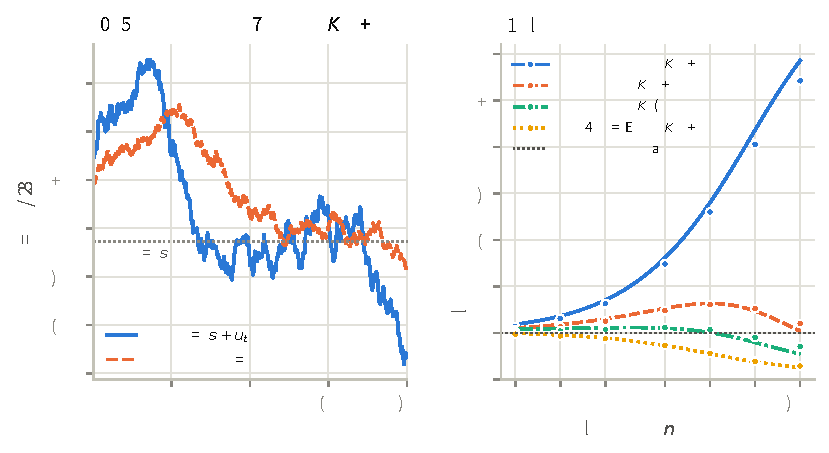
\includegraphics[width=\textwidth]{ch2/ar1.pdf}
  \caption{自相关的状态起伏：评分只能部分追上，窗口胜率比二项分布更分散。(a) 按分匹配（$\sigma_q=100$，$K=16$）中一名实力接近中位数的玩家：当局实力 $s+u_t$ 与评分折算的实力；(b) $n$ 局窗口胜率的人内方差除以二项方差 $\hat p(1-\hat p)/n$，点为模拟（取前 2,000 人的逐局序列，每人 2,000 局切成 $2000/n$ 个窗口），曲线为\cref{eq:ch2-varratio}及随机匹配下的对应公式。参数：10,000 人，$\tau=200$，$\sigma_u=100$，$\rho=0.99$，3000 轮，统计第 1001–3000 局。\tagOwn}
  \label{fig:ch2-ar1}
\end{figure}

\subsection{长期进步：评分滞后，胜率高出期望得分约 $\lambda v/K$}
\label{sec:ch2-improve}

\textbf{假设}：玩家每局实力上升 $v$ 分。\textbf{推导}（\cref{app:ch2-improve}）：由\cref{eq:ch2-identity}，$W-\bar E$ 精确等于评分上升速度除以 $K$。稳态下评分折算的实力与真实实力同速上升，评分以 $\lambda v$ 的速度上升，于是
\begin{equation}
  W-\bar E\approx\frac{\lambda v}{K},\qquad \text{滞后（实力分）}\approx\frac{4\lambda v}{Kc}=\lambda v\cdot\frac{4}{Kc}.
  \label{eq:ch2-improve}
\end{equation}
\textbf{模拟}（\cref{fig:ch2-improve}）：系统平稳后随机抽 2\% 玩家每局进步 $v$，共进步 300 分。按分匹配（$\sigma_q=100$）下，$K=16$ 时 $v=0.25,0.5,1.0$ 的 $W-\bar E$ 为 1.79、3.54、6.67 个百分点，公式（$\lambda^*=1.17$）为 1.82、3.64、7.29；$K=32$ 时为 1.11、2.19、4.40，公式为 1.10、2.20、4.41；$v=0.5$ 的滞后为 28.9 分（$K=16$，公式 25.3）和 15.0 分（$K=32$，公式 15.3）\tagOwn。$v=1$、$K=16$ 时偏低约 9\%，可能的原因是进步者升到高分区后同分对手变少，评分上升受窗口边缘限制。若让 10\% 的玩家同时进步（$v=0.5$），测得的 $W-\bar E$ 会再低 11\%–15\%：进步者之间频繁对局，零和更新不给这一群体带来净分\tagOwn。

真实数据里有对应的痕迹：TrueSkill~2 在 Halo~5 数据中发现，新玩家前 10 局的实际胜率（45\%–47\%）低于经典 TrueSkill 的预测（48\%–49\%），作者把它解释为实力随经验上升、而模型假设实力只做无偏随机游走，并据此加入经验偏移\cite{minka2018trueskill}\tagLit。这正是\cref{eq:ch2-identity}的另一面：胜率与预测胜率的差，衡量的是评分没跟上实力变化的部分。Düring 等人用动理学方程研究了带学习效应的 Elo 模型\cite{during2019boltzmann}\tagLit。

\begin{figure}[htbp]
  \centering
  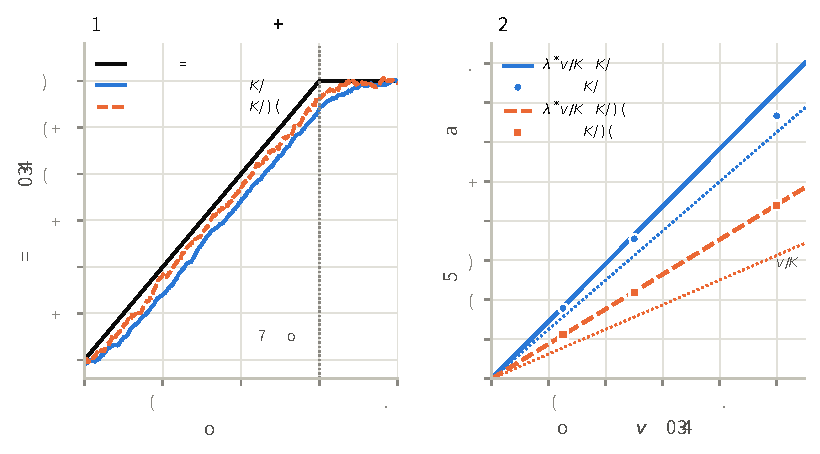
\includegraphics[width=\textwidth]{ch2/improve.pdf}
  \caption{长期进步：评分滞后，胜率高出期望得分。(a) 每局进步 $0.5$ 分的玩家：真实实力增量与评分折算的实力增量；(b) 斜坡第 101 局至结束的 $W-\bar E$，点为模拟，实线为\cref{eq:ch2-improve}（$\lambda^*$ 取 $\sigma_q=100$ 的平稳值），点线为 $v/K$。参数：10,000 人，$\tau=200$，按分匹配 $\sigma_q=100$，系统运行 1000 轮后随机抽 200 人每局进步 $v$、共 $+300$ 分，之后再观察 200 局。\tagOwn}
  \label{fig:ch2-improve}
\end{figure}

\textbf{小结}：实力在变化时，期望胜率仍可写成 $W(t)\approx\bar E(t)+\lambda v(t)/K+\tfrac c4(1-a)u_t$：第一项由匹配决定，第二项来自长期进步，第三项来自没被评分吸收的状态。能算的是期望；不确定性要在二项误差之外乘以\cref{eq:ch2-varratio}的修正因子。

% ======================================================================
\section[统计不确定性：分辨 52\% 与 50\% 约需 4,900 局]{统计不确定性：分辨 52\% 与 50\%\\约需 4,900 局}
\label{sec:ch2-stats}

真实胜率为 $p$ 时，$n$ 局胜率的标准误为 $\sqrt{p(1-p)/n}$：$p=0.5$ 时 20 局 $\pm11.18$、100 局 $\pm5.00$、500 局 $\pm2.24$ 个百分点（一倍标准误）\tagOwn。小样本的区间应使用 Wilson 区间而不是 Wald 区间\cite{wilson1927probable,brown2001interval}\tagLit\needcheck[（Wilson 1927 与 Brown–Cai–DasGupta 2001 只核对了书目信息）]。

\begin{table}[htbp]
  \centering\small
  \caption{观测胜率的不确定性（各局独立）。Wald 半宽按 $p=0.5$ 计算；末列为观测胜率恰为 52\% 时的 Wilson 95\% 区间。\tagOwn}
  \label{tab:ch2-ci}
  \begin{tabular}{rrrr}
    \toprule
    局数 $n$ & 标准误 & 95\% 半宽（Wald） & 观测 52\% 时的 Wilson 区间\\
    \midrule
    20 & 11.18 & $\pm21.9$ & 31.6\%–71.7\%\\
    50 & 7.07 & $\pm13.9$ & 38.5\%–65.2\%\\
    100 & 5.00 & $\pm9.8$ & 42.3\%–61.5\%\\
    200 & 3.54 & $\pm6.9$ & 45.1\%–58.8\%\\
    500 & 2.24 & $\pm4.4$ & 47.6\%–56.3\%\\
    1,000 & 1.58 & $\pm3.1$ & 48.9\%–55.1\%\\
    2,000 & 1.12 & $\pm2.2$ & 49.8\%–54.2\%\\
    5,000 & 0.71 & $\pm1.4$ & 50.6\%–53.4\%\\
    \bottomrule
  \end{tabular}
\end{table}

\textbf{所需局数}。检验 $H_0\colon p=p_0$ 对 $p=p_1$，双侧显著性 $\alpha$、检验力 $1-\beta$ 所需局数为（正态近似，\cref{app:ch2-sample}）
\begin{equation}
  n=\Biggl(\frac{z_{1-\alpha/2}\sqrt{p_0(1-p_0)}+z_{1-\beta}\sqrt{p_1(1-p_1)}}{p_1-p_0}\Biggr)^2.
  \label{eq:ch2-samplesize}
\end{equation}
区分 52\% 与 50\%：$\alpha=0.05$ 双侧、检验力 80\% 需要 4,903 局；单侧 3,862 局；检验力 90\% 需要 6,563 局。若观测胜率恰为 52\%，要让 Wilson 95\% 区间不含 50\%，至少需要 2,401 局\tagOwn。纯运气也会制造“高胜率”：真实 50\% 时，100 局中胜率不低于 60\% 的概率为 2.84\%，20 局中至少 14 胜为 5.77\%、至少 15 胜为 2.07\%，500 局中不低于 55\% 为 1.42\%\tagOwn。玩家基数一大，总有不少人只凭运气就有一段漂亮战绩。

\textbf{相关性会改变误差}（\cref{fig:ch2-ci}(a)）：把\cref{eq:ch2-varratio}的修正因子乘到二项方差上，100 局窗口的 95\% 半宽在按分匹配、实力固定时约为 $\pm7.2$ 个百分点，在随机匹配加状态起伏时约为 $\pm19.7$ 个百分点（相对长期均值），而二项分布为 $\pm9.8$\tagOwn。

\begin{figure}[!tbp]
  \centering
  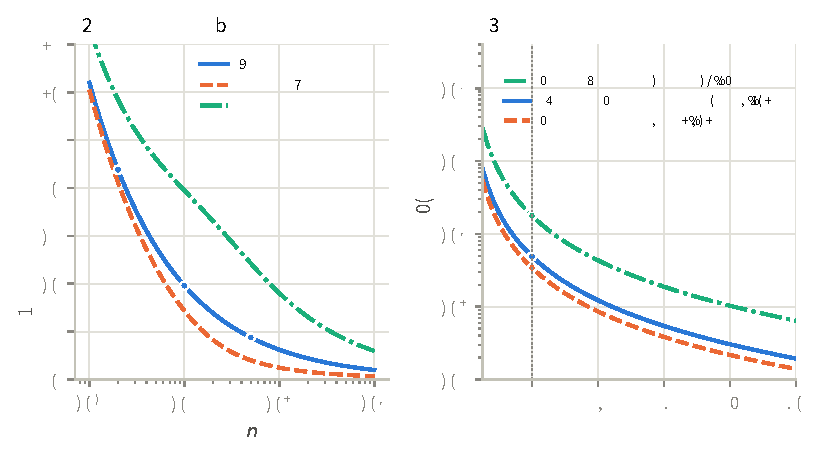
\includegraphics[width=\textwidth]{ch2/ci.pdf}
  \caption{胜率的统计不确定性。(a) 真实胜率 50\% 时 $n$ 局观测胜率的 95\% 区间半宽：二项分布（三个点为 20、100、500 局），以及按\cref{eq:ch2-varratio}修正后的按分匹配（实力固定，$\sigma_q=100$，$K=16$）和随机匹配加 AR(1) 状态（$\sigma_u=100$，$\rho=0.99$）；(b) 双侧 $\alpha=0.05$、检验力 80\% 时区分“五五开”所需局数，8 人局的第一名率与平均名次按 Plackett–Luce 换算到相同的实力优势。\tagOwn}
  \label{fig:ch2-ci}
\end{figure}

\textbf{8 人局}（\cref{fig:ch2-ci}(b)）：前四率是 $p_0=0.5$ 的二项比例，区分 52\% 与 50\% 同样要 4,903 局；第一名率要对 12.5\% 检验，在 Plackett–Luce 下同等实力优势（前四率 52\% 对应 $d\approx11$ 分）的第一名率只有 13.2\%，需要约 17,700 局；平均名次在同水平时的标准差为 $\sqrt{(N^2-1)/12}=2.29$，检测平均名次移动 0.10（4.5→4.4）需要约 4,100 局，而前四率 52\% 的玩家平均名次为 4.39，用平均名次检验只需约 3,400 局\tagOwn。名次本身比“是否进前四”包含更多信息，估计 8 人局实力时应优先用完整名次。


\FloatBarrier
% ======================================================================
\section{小结：胜率能不能算、和什么有关}
\label{sec:ch2-summary}

\Cref{tab:ch2-summary} 汇总本章结论。总的回答是：在“只有输赢、匹配不被操纵”的前提下，胜率可以算，但要先说清三件事——对手从哪里来（随机还是按分）、“胜”指什么（1v1、团队还是名次）、实力是固定还是在变。

\begin{table}[!htbp]
  \centering\footnotesize
  \caption{影响长期胜率的因素：方向与量级（模型参数见各节，$\tau=200$，$K=16$ 除非另注）。\tagOwn}
  \label{tab:ch2-summary}
  \renewcommand{\arraystretch}{1.15}
  \begin{tabularx}{\textwidth}{>{\raggedright\arraybackslash}p{2.6cm}>{\raggedright\arraybackslash}X>{\raggedright\arraybackslash}p{5.2cm}}
    \toprule
    因素 & 方向 & 量级\\
    \midrule
    自身实力（随机匹配） & 实力百分位越高胜率越高，$W=\Phi(r z_q)$ & 最强/最弱 10\%：83\% / 17\%\\
    群体离散度 $\tau$ & 越大胜率越极端 & $\tau$=100→300：前 10\% 由 72\% 到 88\%\\
    游戏随机性 & 越随机越接近 50\%，评分差同比例压缩 & 单局噪声 150：斜率 ×0.81，前 10\% 79\%\\
    匹配规则 & 按分匹配把胜率压向 50\%，窗口越窄越接近 & 十分位范围：随机 17–83\%，$\sigma_q$=100 时 42–58\%，$\sigma_q$=20 时 49–51\%\\
    匹配时的评分/段位 & 只通过对手分布起作用；评分落后于实力时胜率偏高 & 重置的高手前 50 局 77.5\%，约 47 局追回一半\\
    $K$ 因子 & 不改变随机匹配的胜率；决定评分噪声与滞后 & $\sigma_e\approx9.3\sqrt K$；误差衰减 55–65 局（$K$=16）、30–34 局（$K$=32）\\
    每队人数 $n$ & 个人优势被稀释 & $n$=5：斜率为 1v1 的 0.40（加和）或 0.23（均值）\\
    每局人数 $N$ 与“胜”的定义 & 基准率 $1/N$（第一名）或 50\%（前一半） & 8 人局按分匹配：第一名 12.5\%，前四 50\%，平均名次 4.5\\
    独立的单局波动 & 等于游戏更随机 & 见“游戏随机性”\\
    自相关的状态 & 长期胜率几乎不变，窗口胜率更分散 & 百局方差为二项的 1.6 倍（按分）至 3.6 倍（随机）（模拟）\\
    长期进步 & 胜率高于预测胜率 & $W-\bar E\approx\lambda v/K$：$v$=0.5 时约 3.5 个百分点\\
    样本量 & 决定能否分辨 & 52\% 对 50\%：4,903 局（80\% 检验力）\\
    \bottomrule
  \end{tabularx}
\end{table}

\begin{keybox}[本章要点：带到后面两章的三点]
\begin{enumerate}
\item 按分匹配下长期胜率接近 50\% 是\cref{eq:ch2-identity}的直接结果，不需要任何“控胜率”机制来解释；有没有操纵要看匹配输入（\cref{ch:streaks}）。
\item 状态起伏让窗口胜率比二项分布更分散，这是\cref{ch:streaks}讨论连败与“上头”的起点。
\item 从训练的角度看，胜负标签在系统稳定后仍然源源不断，但信息集中在偏离预测的部分（$y-E$），这与\cref{ch:ml}讨论的“目标是胜率还是实力”直接相关。对酒馆战棋这类 8 人名次游戏，评估实力时应使用完整名次而不是前四率，并对固定参照池而不是天梯对手来测量。
\end{enumerate}
\end{keybox}



\chapter{研究三：诚实系统会不会制造“Elo 感”}
\label{ch:streaks}
% 由章节写作者填写

\chapter{研究四：训练视角——目标是胜率还是实力}
\label{ch:ml}
% 由章节写作者填写

% 结论与展望：整合阶段撰写（含后续计划：社交平台阴谋论收集与检验、个人对局数据分析，见 docs/ROADMAP.md）
\chapter*{结论与展望}
\addcontentsline{toc}{chapter}{结论与展望}
（待整合阶段撰写。）

\printbibliography[heading=bibintoc,title=参考文献]
\appendix
% 附录：各章较长的推导、模拟参数表放在各自的 appendix_chN.tex 中（每章一个 \section，标签 app:chN-...）
\chapter{推导与模拟细节}
\label{app}
% 第一章附录：两部分各自的附录
% 第一章（1a）附录：本部分正文引用的推导
\section{第一章学术部分的推导}\label{app:ch1a}

\subsection{正态曲线与 Elo 逻辑斯蒂曲线的刻度换算}\label{app:ch1a-scale}

Elo 曲线\cref{eq:1a-elo-curve} 在分差 0 处的斜率为 $\Elogit'(0)=\cElo/4=\ln 10/1600\approx 1.439\times10^{-3}$（每分）。正态曲线 $\Phi\big(x/(\sigma\sqrt2)\big)$ 在 0 处的斜率为 $1/(\sigma\sqrt2\sqrt{2\pi})$。令两者相等，得
\[
  \sigma=\frac{1600}{\ln 10\cdot\sqrt{2}\cdot\sqrt{2\pi}}\approx 196 ,
\]
即“400 分刻度的逻辑斯蒂曲线”在中心附近等价于“每人单局表现标准差约 196 分”的正态曲线，与 Elo 原书取的 200 几乎相同\tagOwn。用 FIDE 现行条例 8.1.1 表（$p=0.51,\dots,0.99$ 共 49 格）做最小二乘拟合，得到的单人标准差为 202.6；表中分差与 $\sigma=200$ 的正态曲线最大相差 19 分（$p=0.99$ 处），与 Elo 逻辑斯蒂曲线最大相差 121 分（同一处）\tagOwn。两种曲线在中段几乎重合，差别只在 $p>0.9$ 的尾部：逻辑斯蒂曲线给弱者留的胜率更大。

\subsection{TrueSkill 两人更新式}\label{app:ch1a-ts}

设胜方、负方实力的先验为 $s_{\mathrm w}\sim\Normal(\mu_{\mathrm w},\sigma_{\mathrm w}^2)$、$s_{\mathrm l}\sim\Normal(\mu_{\mathrm l},\sigma_{\mathrm l}^2)$，表现 $p=s+\Normal(0,\beta^2)$。表现差 $d=p_{\mathrm w}-p_{\mathrm l}\sim\Normal(m,c^2)$，其中 $m=\mu_{\mathrm w}-\mu_{\mathrm l}$，$c^2=\sigma_{\mathrm w}^2+\sigma_{\mathrm l}^2+2\beta^2$。观测到“胜方获胜且不是平局”即 $d>\varepsilon$。

\paragraph{截断正态的矩。}记 $d=m+cZ$，$Z$ 为标准正态，$t=m/c$，$a=\varepsilon/c$，则 $d>\varepsilon\Leftrightarrow Z>-(t-a)$。对 $u=t-a$，
\[
  \E[Z\mid Z>-u]=\frac{\varphi(u)}{\Phi(u)}=:v(t,a),\qquad
  \Var[Z\mid Z>-u]=1-v(t,a)\big(v(t,a)+u\big)=:1-w(t,a).
\]
\paragraph{传回实力。}$(s_{\mathrm w},d)$ 联合正态，$\Cov(s_{\mathrm w},d)=\sigma_{\mathrm w}^2$，故 $\E[s_{\mathrm w}\mid d]=\mu_{\mathrm w}+(\sigma_{\mathrm w}^2/c^2)(d-m)$，$\Var[s_{\mathrm w}\mid d]=\sigma_{\mathrm w}^2(1-\sigma_{\mathrm w}^2/c^2)$。对条件 $d>\varepsilon$ 取期望（全期望与全方差公式）：
\[
  \E[s_{\mathrm w}\mid d>\varepsilon]=\mu_{\mathrm w}+\frac{\sigma_{\mathrm w}^2}{c}\,v(t,a),\qquad
  \Var[s_{\mathrm w}\mid d>\varepsilon]=\sigma_{\mathrm w}^2\Big(1-\frac{\sigma_{\mathrm w}^2}{c^2}\Big)+\frac{\sigma_{\mathrm w}^4}{c^4}\,c^2\big(1-w\big)
  =\sigma_{\mathrm w}^2\Big(1-\frac{\sigma_{\mathrm w}^2}{c^2}\,w(t,a)\Big).
\]
负方的 $\Cov(s_{\mathrm l},d)=-\sigma_{\mathrm l}^2$，均值更新取负号，方差更新形式相同。TrueSkill 把后验近似为具有这两个矩的高斯（期望传播中的矩匹配），即得\cref{eq:1a-ts-update}。若有动态方差 $\gamma^2$（TrueSkill 论文的记号），赛前先令 $\sigma^2\leftarrow\sigma^2+\gamma^2$。爆冷时 $t\ll0$，$v\approx a-t$ 很大，均值更新幅度近似与“爆冷程度”成正比；$t\gg0$（强者赢弱者）时 $v\to0$，几乎不更新\tagOwn。

\subsection{TrueSkill 匹配质量即相对平局概率}\label{app:ch1a-quality}

平局边际 $\varepsilon$ 很小时，$\Prob(|d|\le\varepsilon)\approx 2\varepsilon\cdot\frac{1}{c\sqrt{2\pi}}\exp\!\big(-\frac{m^2}{2c^2}\big)$。它的最大可能值出现在 $m=0$ 且双方实力完全确定（$\sigma_i=\sigma_j=0$，$c^2=2\beta^2$）时，为 $2\varepsilon/\big(\sqrt{2\beta^2}\sqrt{2\pi}\big)$。两者之比与 $\varepsilon$ 无关：
\[
  q_{\text{draw}}=\sqrt{\frac{2\beta^2}{c^2}}\exp\!\Big(-\frac{m^2}{2c^2}\Big),\qquad c^2=2\beta^2+\sigma_i^2+\sigma_j^2 ,
\]
即\cref{eq:1a-ts-quality}。它同时惩罚均值差（指数项）和不确定性（根号项）：两个新号即使均值相同，质量也低于两个均值相同的老玩家\tagOwn。

\subsection{EOMM 的三种特例}\label{app:ch1a-eomm}

设玩家流失只取决于本局结果，记 $c(\mathrm W)$、$c(\mathrm L)$、$c(\mathrm D)$ 为胜、负、平后的流失概率，$P_{ij}(\cdot)$ 为 $i$ 对 $j$ 的结果分布。一对玩家的流失之和为
\[
  P_{ij}(\mathrm W)\big[c(\mathrm W)+c(\mathrm L)\big]+P_{ij}(\mathrm L)\big[c(\mathrm L)+c(\mathrm W)\big]+P_{ij}(\mathrm D)\cdot 2c(\mathrm D)
  =\big[c(\mathrm W)+c(\mathrm L)\big]-P_{ij}(\mathrm D)\big[c(\mathrm W)+c(\mathrm L)-2c(\mathrm D)\big].
\]
对所有配对求和后，最小化总流失等价于：若 $c(\mathrm W)+c(\mathrm L)>2c(\mathrm D)$，最大化总平局概率；若不等号反向，最小化总平局概率。平局在实力相近时最可能发生，所以前一种情形下按分匹配最优，后一种情形下按分匹配最差。若流失与本局结果无关（只取决于赛前状态），上式与配对无关，任何匹配（包括随机匹配）都一样。这就是 Chen 等\cite{chen2017eomm} 第 4 节的结论。

由此还可以看出一点（\tagOwn 的推论）：在\emph{没有平局}的输赢游戏中，若流失只取决于本局结果，则每对玩家的流失之和恒为 $c(\mathrm W)+c(\mathrm L)$，匹配对总流失毫无影响。参与度优化匹配要有效果，流失必须依赖于玩家的状态（例如最近几局的胜负、技能、在线时长），而且这种依赖要因人而异。EOMM 的输入正是“最近 10 局的胜负平”等状态变量，这也是它与“按连胜连败安排对手”在机制上相通的原因。

\subsection{Yuksel 目标胜率公式}\label{app:ch1a-yuksel}

设玩家最近 $n$ 局赢了 $w$ 局，希望包含接下来 $n+1$ 局在内、长 $2n+1$ 的窗口的期望胜率为 $\lambda$。若接下来每局对手都使其胜率为 $p$，窗口期望胜局数为 $w+(n+1)p$，令其等于 $\lambda(2n+1)$ 即得\cref{eq:1a-yuksel}。两人游戏取 $\lambda=1/2$、论文实验取 $n=5$ 时，$w=0,1,\dots,5$ 对应的目标胜率依次为 $11/12,\,9/12,\,7/12,\,5/12,\,3/12,\,1/12$（约 92\%、75\%、58\%、42\%、25\%、8\%）\tagOwn。论文另取概率窗口 $\Delta p=1/(2n+2)=1/12$，在评分 $f^{-1}(p\pm\Delta p)$ 范围内找对手；这保证 $p-\Delta p>0$ 且 $p+\Delta p<1$\cite{yuksel2024skill}。换言之，这一匹配器对近期战绩的反应相当强：连赢 5 局后，下一局几乎一定会遇到明显更强的对手。

% 第一章（1b）附录


\section{第二章的推导与模拟参数}
\label{app:ch2}

本节给出研究二（\cref{ch:winrate}）中较长的推导和全部模拟设定。记号同正文：$F(x)=1/(1+10^{-x/400})$，$c=\ln10/400$，$F'(x)=c\,F(x)\bigl(1-F(x)\bigr)$，$F'(0)=c/4$；$\sigma_d=1.702/c\approx295.7$。

\subsection{模拟设定}
\label{app:ch2-params}

所有模拟由 \texttt{code/ch2/model.py} 完成（numpy 向量化，固定随机种子），结果缓存在 \texttt{code/ch2/cache/}。共同设定：
\begin{itemize}
\item 玩家实力 $s\sim\Normal(1500,\tau^2)$，默认 $\tau=200$；初始评分全部为 1500（刻度拉伸实验取初始评分等于实力）。
\item 每轮每人恰好一局。标准实验 10,000 人、3,000 轮，前 1,000 轮预热，统计第 1,001–3,000 局（每人 2,000 局，个人胜率的二项标准误约 1.1 个百分点）。
\item 1v1：$p=F(s_i-s_j)$，评分 $R_i\leftarrow R_i+K(y-E)$，$E=F(R_i-R_j)$。
\item 5v5：加和模型 $p=F\bigl((\sum s_A-\sum s_B)/\sqrt5\bigr)$，均值模型 $p=F(\bar s_A-\bar s_B)$；每名队员按团队的 $K(y-E)$ 更新，$E$ 用与结果模型相同的形式。
\item 8 人自由混战：表现 $=s+$Gumbel（尺度 $400/\ln10$），评分按两两比较更新，$\Delta R_i=\frac{K}{7}\sum_{j\ne i}\bigl(S_{ij}-F(R_i-R_j)\bigr)$，$S_{ij}=1$ 表示 $i$ 名次在 $j$ 之前。
\item 匹配：随机匹配为每轮全体随机打乱后依次成组；按分匹配为按 $R+\Normal(0,\sigma_q^2)$ 排序后相邻成组，团队在 10 人组内蛇形分队（按评分排序后 ABBAABBAAB）。不使用任何隐藏变量。
\end{itemize}

\begin{table}[h]
  \centering\small
  \caption{第二章的模拟实验（标准实验均为 10,000 人、3,000 轮、统计第 1,001–3,000 局）。}
  \label{tab:ch2-params}
  \begin{tabularx}{\textwidth}{>{\raggedright\arraybackslash}p{3.4cm}>{\raggedright\arraybackslash}X>{\raggedright\arraybackslash}p{3.2cm}}
    \toprule
    实验 & 设定 & 用于\\
    \midrule
    1v1 随机匹配 & $K=16,32$；另有 $\tau=100,300$；单局噪声 $\sigma_x=150$；AR(1) 状态 $\sigma_u=100$、$\phi=0.99$ & \cref{fig:ch2-three}、\ref{fig:ch2-random}、\ref{fig:ch2-fair}、\ref{fig:ch2-ar1}\\
    1v1 按分匹配 & $\sigma_q=20,50,100,200$，$K=16,32$；另有 $\sigma_q=100$ 加单局噪声或 AR(1) 状态 & \cref{fig:ch2-three}、\ref{fig:ch2-sbmm}、\ref{fig:ch2-error}、\ref{fig:ch2-ar1}\\
    5v5 & 随机分队（加和、均值）；按分匹配 $\sigma_q=100$（加和、均值）、$\sigma_q=200$（加和）；$K=16$ & \cref{fig:ch2-fair}、\ref{fig:ch2-team}\\
    8 人自由混战 & 随机组局、按分匹配 $\sigma_q=100$；$K=16$ & \cref{sec:ch2-ffa}\\
    $K$ 扫描 & 4,000 人，2,500 轮，$K=8$–64，随机匹配与 $\sigma_q=100,200$ & \cref{fig:ch2-error}(a)\\
    重置实验 & 运行 1,000 轮后从实力前 10\% 中重置 500 人为 1500，跟踪 400 局 & \cref{fig:ch2-reset}\\
    刻度拉伸 & 2,000 人，初始评分 $=$ 实力，$K=16$，10,000 轮，$\sigma_q=20,50,100,200$ & \cref{fig:ch2-stretch}\\
    进步实验 & 运行 1,000 轮后随机抽 2\%（对照：10\%）玩家每局进步 $v=0.25,0.5,1$，共 $+300$，再观察 200 局；$\sigma_q=100$ & \cref{fig:ch2-improve}\\
    \bottomrule
  \end{tabularx}
\end{table}

\subsection{随机匹配与团队胜率}
\label{app:ch2-random}

\textbf{高斯恒等式。}设 $Z,Z'$ 独立标准正态。$\E[\Phi(a+bZ)]=\E[\Prob(Z'\le a+bZ\mid Z)]=\Prob(Z'-bZ\le a)=\Phi(a/\sqrt{1+b^2})$。取 $Z=(t-\mu)/\tau$、$a=(s-\mu)/\sigma_d$、$b=-\tau/\sigma_d$，即得\cref{eq:ch2-random}。数值表（\cref{tab:ch2-tau}、\ref{tab:ch2-team}）不用正态近似，而是用 80 点 Gauss–Hermite 求积直接计算 $\E[F(X)]$；“前 10\% 平均”对第 90–100 百分位的 20,001 个等距百分位点求平均。

\textbf{团队。}焦点玩家实力 $\mu+d$，$n-1$ 名队友与 $n$ 名对手独立取自 $\Normal(\mu,\tau^2)$。加和模型下 $\sum s_A-\sum s_B=d+\sum_{i=1}^{n-1}(t_i-\mu)-\sum_{j=1}^{n}(o_j-\mu)$，均值为 $d$、方差 $(2n-1)\tau^2$，除以 $\sqrt n$ 得 $X\sim\Normal(d/\sqrt n,(2n-1)\tau^2/n)$；均值模型除以 $n$。再套用高斯恒等式得\cref{eq:ch2-team}。$d=0$ 处的斜率：加和模型 $\phi(0)\big/\bigl(\sqrt n\sqrt{\sigma_d^2+(2n-1)\tau^2/n}\bigr)$，$n$ 大时 $\approx\phi(0)/\bigl(\sqrt n\sqrt{\sigma_d^2+2\tau^2}\bigr)$；均值模型 $\phi(0)\big/\bigl(n\sqrt{\sigma_d^2+(2n-1)\tau^2/n^2}\bigr)\approx\phi(0)/(n\sigma_d)$。

\subsection{“五五开”对局的真实胜率}
\label{app:ch2-fair}

设 $s\sim\Normal(\mu,\tau^2)$，$R=s+e$，$e\sim\Normal(0,\sigma_e^2)$ 独立。由正态共轭，$s\mid R\sim\Normal\bigl(\mu+\tfrac{\tau^2}{\tau^2+\sigma_e^2}(R-\mu),\,v\bigr)$，$v=\tau^2\sigma_e^2/(\tau^2+\sigma_e^2)$。两名评分同为 $r$ 的玩家，实力条件独立且均值相同，故 $\Delta s=s_A-s_B\sim\Normal(0,2v)$，与 $r$ 无关。令 $p=F(\Delta s)$，$x=F^{-1}(p)$，$\dd p/\dd x=c\,p(1-p)$，换元得
\[
  f_p(p)=\frac{1}{\sigma_\Delta}\phi\Bigl(\frac{F^{-1}(p)}{\sigma_\Delta}\Bigr)\cdot\frac{1}{c\,p(1-p)},\qquad \sigma_\Delta=\sqrt{2v}.
\]
$p$ 的分位数为 $F(z_q\sigma_\Delta)$。团队加和模型下，给定两队评分和相等，$(\sum s_A-\sum s_B)/\sqrt n$ 的方差为 $2nv/n=2v$，只是 $v$ 中的 $\sigma_e$ 换成团队游戏的个人评分误差。

\subsection{恒等式与评分误差的线性化}
\label{app:ch2-linear}

\textbf{恒等式}：$R_T-R_0=\sum_t\Delta R_t=K\sum_t(y_t-E_t)$，除以 $KT$ 即得\cref{eq:ch2-identity}；不需要任何模型假设，只要求每局更新恰为 $K(y_t-E_t)$。

\textbf{稳态误差。}按分匹配下对手评分 $R'\approx R$。令 $e=R-s$、$e'=R'-s'$，则 $y-E=\bigl[F(s-s')-F(R-R')\bigr]+\eta$，$\eta=y-F(s-s')$ 满足 $\E\eta=0$、$\Var\eta=p(1-p)\approx\tfrac14$。线性化 $F(s-s')-F(R-R')\approx-\tfrac c4(e-e')$，记 $k=Kc/4$：
\[
  e_{t+1}=(1-k)e_t+k\,e'_t+K\eta_t .
\]
设 $e,e',\eta$ 两两独立、$\Var e=\Var e'=V$，平稳时 $V=(1-k)^2V+k^2V+K^2/4$，解得
\[
  V=\frac{K^2}{8k(1-k)}=\frac{K}{2c\,(1-Kc/4)} .
\]
略去对手误差（$e'\equiv0$）则为 $V=K^2/\bigl(4(2k-k^2)\bigr)\approx K/(2c)$，即\cref{tab:ch2-sigmae}的第二列。评分刻度为 $\lambda$ 时，实力差 $=(R-R'-e+e')/\lambda$，回复系数变为 $k_\lambda=Kc/(4\lambda)$，于是 $V=K\lambda/\bigl(2c(1-Kc/(4\lambda))\bigr)$，这就是按分匹配下误差略大的原因。

\textbf{时间常数。}理想情况下误差每局衰减 $1-k$，时间常数 $1/k=4/(Kc)\approx695/K$。一般情形需要两处修正。其一，线性化斜率应取 $F'$ 在实际实力差上的平均，即 $c\,\E[P(1-P)]=\tfrac c4\cdot4\E[P(1-P)]$。其二，在\cref{app:ch2-edge}的窗口模型下，玩家的期望评分变化为
\[
  \E[\Delta R]\approx K\tfrac c4\bigl[(s-\mu)-(1-g+bg)(R-\mu)\bigr],\qquad b=\frac{\lambda\tau^2}{\sigma_R^2},
\]
其中 $bg$ 来自“配到的对手评分向均值回归，其实力又按 $b$ 回归”。把 $R-\mu=\lambda(s-\mu)+e$ 代入，$e$ 的系数为 $-K\tfrac c4\bigl(1-g(1-b)\bigr)=-K\tfrac c4\cdot\frac{\lambda\tau^2+\sigma_q^2}{\sigma_R^2+\sigma_q^2}$。合并两处得 $\tau_R=4/(Kc\kappa)$，$\kappa=4\E[P(1-P)]\cdot(\lambda\tau^2+\sigma_q^2)/(\sigma_R^2+\sigma_q^2)$。随机匹配时 $\sigma_q\to\infty$，$\kappa\to4\E[P(1-P)]$，但 $\E[P(1-P)]$ 因人而异（实力越极端越小），群体的误差自相关是各人指数衰减的平均，\cref{fig:ch2-error}(b) 的随机匹配虚线即按此计算。

\subsection{匹配窗口的边缘效应}
\label{app:ch2-edge}

设评分在群体中近似正态，均值 $\mu$、方差 $\sigma_R^2=\lambda^2\tau^2+\sigma_e^2$。排序键 $k=R+\xi$，$\xi\sim\Normal(0,\sigma_q^2)$；人口足够多时，相邻者的键几乎相等。由正态共轭，$R'\mid k\sim\Normal\bigl(\mu+g(k-\mu),\,g\sigma_q^2\bigr)$，$g=\sigma_R^2/(\sigma_R^2+\sigma_q^2)$。给定自己的 $R$，$k=R+\xi$，于是 $R'\mid R\sim\Normal\bigl(\mu+g(R-\mu),\,g^2\sigma_q^2+g\sigma_q^2\bigr)$，即
\[
  R-R'\sim\Normal\bigl((1-g)(R-\mu),\ g(1+g)\sigma_q^2\bigr).
\]
平稳时 $\Delta R/(KT)\to0$，长期胜率等于平均预测胜率 $\bar E=\E[F(R-R')]$，用 $F\approx\Phi(\cdot/\sigma_d)$ 和高斯恒等式得\cref{eq:ch2-edge}。计算时 $\lambda$ 取平稳值 $\lambda^*$（\cref{app:ch2-stretch}），$\sigma_e$ 取 $\sigma_e(K,\lambda^*)$；十分位平均对评分标准化位置 $z\in$ 最高 10\% 求平均。配对两人评分差的方差为 $2g\sigma_q^2$（两人的 $\xi$ 在给定相同键时各有条件方差 $g\sigma_q^2$，条件均值相同）。

\subsection{刻度拉伸}
\label{app:ch2-stretch}

\textbf{精确结论。}若一局双方评分相等，则 $E=\tfrac12$，赛后两人评分为 $R\pm K/2$，两人评分平方和增加 $K^2/2$，平均每人 $K^2/4$；均值不变，所以群体评分方差每局增加 $K^2/4$。更一般地，只要给定自己的评分时对手实力与自己的实力可交换，就有 $\E[y-E\mid R]=0$，进而 $\Cov(R,y-E)=0$，于是 $\Var(R_{t+1})=\Var(R_t)+K^2\Var(y-E)$，方差只增不减。真实实力分布不变，排序又近乎正确，增加的方差只能表现为斜率 $\lambda$ 变大：$\lambda^2\tau^2\approx\lambda_0^2\tau^2+K^2t/4$。

\textbf{平均场方程。}沿用\cref{app:ch2-linear}的期望评分变化，把它投影到 $s$ 上：
\[
  \frac{\dd\lambda}{\dd t}=\frac{\Cov(\E[\Delta R],s)}{\tau^2}=K\tfrac c4\bigl[1-(1-g+bg)\lambda\bigr].
\]
代入 $g$、$b$ 化简：$1-(1-g(1-b))\lambda=\bigl[\sigma_R^2+\sigma_q^2-\lambda\sigma_q^2-\lambda^2\tau^2\bigr]/(\sigma_R^2+\sigma_q^2)=\bigl[\sigma_e^2+\sigma_q^2(1-\lambda)\bigr]/(\lambda^2\tau^2+\sigma_e^2+\sigma_q^2)$，即\cref{eq:ch2-stretch}。令分子为零得 $\lambda^*=1+\sigma_e^2(\lambda^*)/\sigma_q^2$；由于 $\sigma_e^2(\lambda)\approx\lambda\,\sigma_e^2(1)$，解得 $\lambda^*=1/\bigl(1-\sigma_e^2(1)/\sigma_q^2\bigr)$，仅当 $\sigma_q>\sigma_e(1)$ 时为正。$\sigma_q\to0$ 时方程化为 $\dd\lambda/\dd t\approx K\tfrac c4\sigma_e^2/(\lambda^2\tau^2)=K^2/(8\lambda\tau^2)$，与精确结论一致。\Cref{fig:ch2-stretch} 的虚线用步长 1 局的欧拉法积分这一方程，$\sigma_e^2$ 取 $K\lambda/\bigl(2c(1-Kc/(4\lambda))\bigr)$。

\subsection{团队与自由混战的评分误差、Plackett–Luce 名次}
\label{app:ch2-team}

\textbf{Gumbel 表现与 Plackett–Luce。}设表现 $X_i=s_i+bG_i$，$G_i$ 独立标准 Gumbel，$b=400/\ln10$。标准 Gumbel 满足 $e^{-G}\sim$ 指数分布（率 1），所以 $Y_i=e^{-X_i/b}=e^{-s_i/b}e^{-G_i}$ 服从率为 $w_i=e^{s_i/b}=10^{s_i/400}$ 的指数分布，且“表现最高”等价于“$Y$ 最小”。独立指数变量中 $Y_i$ 最小的概率为 $w_i/\sum_jw_j$；由无记忆性，最小值的大小与“谁最小”独立，去掉第一名后其余人仍是同样的结构，所以完整名次是依次按 worth 比例抽取的 Plackett–Luce 模型。$N=2$ 时 $w_i/(w_i+w_j)=F(s_i-s_j)$，即两两边际恰为 Elo 曲线。焦点玩家 worth 为 $w$、其余 $N-1$ 人为 1 时，第 $j+1$ 次抽取（$j=0,\dots,k-1$）没有抽中焦点玩家的条件概率为 $(N-1-j)/(w+N-1-j)$，连乘取补即得\cref{eq:ch2-pl}。

\textbf{自由混战的评分误差。}同水平的 $N$ 人一局，名次均匀分布，$\sum_jS_{ij}=N-\text{名次}$ 的方差为 $(N^2-1)/12$；步长 $K/(N-1)$ 使单局评分变化方差为 $K^2(N^2-1)/\bigl(12(N-1)^2\bigr)=K^2(N+1)/\bigl(12(N-1)\bigr)$。每局的回复力为 $\frac{K}{N-1}\sum_jF'(0)=K\tfrac c4$，与 1v1 相同，故方差之比为 $\frac{(N+1)/(12(N-1))}{1/4}=\frac{N+1}{3(N-1)}$，$N=8$ 时为 0.43，标准差之比 0.65。

\textbf{团队中的个人评分误差（粗略）。}加和模型下个人评分误差 $e$ 对团队评分差的贡献为 $e/\sqrt n$，回复系数变为 $Kc/(4\sqrt n)$；忽略其余 9 人的误差相关，套用\cref{app:ch2-linear}得 $V\approx K\sqrt n/\bigl(2c(1-\sqrt nKc/4)\bigr)$，$n=5$、$K=16$ 时标准差 57.2，模拟 57.7。均值模型的回复系数为 $Kc/(4n)$，误差更大。

\subsection{状态起伏与窗口胜率的方差}
\label{app:ch2-ar1}

\textbf{评分对状态的吸收。}在实力单位下把评分写成 $\hat s_t=(1-\alpha)\hat s_{t-1}+\alpha(s+u_t)+$噪声，$\alpha=1/\tau_R$。状态部分 $x_t=\sum_{i\ge0}\alpha(1-\alpha)^iu_{t-i}$。$u$ 为 AR(1)，$\Cov(u_{t-i},u_t)=\sigma_u^2\phi^i$，故
\[
  \Cov(x_t,u_t)=\alpha\sigma_u^2\sum_i\bigl[(1-\alpha)\phi\bigr]^i=\frac{\alpha\sigma_u^2}{1-(1-\alpha)\phi},
\]
即\cref{eq:ch2-absorb}。记 $a_0=1-\alpha$，$x$ 的自协方差可以递推得到：$\gamma_x(0)=\alpha^2\sigma_u^2(1+a_0\phi)/\bigl((1-a_0^2)(1-a_0\phi)\bigr)$，$k\ge1$ 时
\[
  \gamma_x(k)=a_0^k\gamma_x(0)+\frac{\alpha^2\sigma_u^2}{1-a_0\phi}\cdot\frac{\phi\,(\phi^k-a_0^k)}{\phi-a_0}.
\]

\textbf{按分匹配下的窗口方差。}由\cref{eq:ch2-identity}，$n$ 局窗口胜率 $W_n=\bar E_n+(R_{t+n}-R_t)/(Kn)$。第一项的局间波动来自窗口内对手评分的随机性，方差约 $\Var(E_t)/n$，其中 $\Var(E_t)=\Var\bigl(F(R-R')\bigr)$ 按\cref{app:ch2-edge}的 $R-R'$ 分布计算（$\sigma_q=100$、$K=16$ 时约 0.026）。第二项的方差为 $2[\Gamma(0)-\Gamma(n)]/(K^2n^2)$，评分（评分单位）的自协方差取 $\Gamma(k)=\lambda^2\gamma_x(k)+\sigma_e^2(1-\alpha)^k$，前者是对状态的跟踪，后者是评分噪声。除以二项方差 $p(1-p)/n\approx1/(4n)$ 即得\cref{eq:ch2-varratio}。模拟中的方差比是“每人 $m=2000/n$ 个连续窗口的样本方差”，期望值为 $\frac{m}{m-1}\bigl[D(n)-D(mn)/m^2\bigr]$，$D(h)=2[\Gamma(0)-\Gamma(h)]$；\cref{fig:ch2-ar1}(b) 的曲线已含此修正，\cref{fig:ch2-ci}(a) 取 $m\to\infty$。$\alpha$ 用修正后的时间常数，$\lambda$、$\sigma_e$ 用平稳值 $\lambda^*$、$\sigma_e(K,\lambda^*)$，均不由模拟拟合。实力固定（$\sigma_u=0$）且 $n\gg\tau_R$ 时，$\Var(R_{t+n}-R_t)\to2\sigma_e^2$，$\mathrm{sd}(W_n)\approx\sqrt2\sigma_e/(Kn)$。

\textbf{随机匹配下的窗口方差。}此时胜负与评分无关，单局胜率 $p_t\approx p(s)+\beta(s)u_t$，$\beta(s)$ 为随机匹配胜率曲线在 $s$ 处的斜率（对手的状态并入对手实力的离散，$\tau\to\sqrt{\tau^2+\sigma_u^2}$）。$n$ 局状态均值的方差为
\[
  V_n=\frac{\sigma_u^2}{n}\Bigl[\frac{1+\phi}{1-\phi}-\frac{2\phi(1-\phi^n)}{n(1-\phi)^2}\Bigr],
\]
方差比约为 $1+n\beta^2V_n/\bigl(p(1-p)\bigr)$，再对实力分布取平均，并作同样的样本方差修正。

\subsection{进步时的胜率与滞后}
\label{app:ch2-improve}

实力以 $v$ 每局上升，评分折算的实力 $\hat s=\mu+(R-a)/\lambda$ 的差距 $g=s-\hat s$ 满足 $\dd g/\dd t=v-\frac{1}{\lambda}\frac{\dd R}{\dd t}$，而 $\frac{\dd R}{\dd t}\approx K\frac c4g$。于是 $g$ 以时间常数 $4\lambda/(Kc)$ 趋于 $g^*=4\lambda v/(Kc)$；稳态时 $\hat s$ 与 $s$ 同速，$\dd R/\dd t=\lambda v$，由\cref{eq:ch2-identity}得 $W-\bar E=\lambda v/K$。这里忽略了窗口回归（会使滞后略大）和零和池中其他玩家的下沉。

\subsection{样本量与 8 人局指标}
\label{app:ch2-sample}

\cref{eq:ch2-samplesize}是比例检验的正态近似。Wilson 区间为
\[
  \Bigl[\hat p+\frac{z^2}{2n}\pm z\sqrt{\frac{\hat p(1-\hat p)}{n}+\frac{z^2}{4n^2}}\Bigr]\Big/\Bigl(1+\frac{z^2}{n}\Bigr).
\]
8 人局同水平时名次均匀，平均名次的方差为 $(N^2-1)/12=5.25$；检验平均名次时用 $n=\bigl((z_{1-\alpha/2}\sigma_0+z_{1-\beta}\sigma_1)/\delta\bigr)^2$，$\sigma_0=2.29$，$\sigma_1$ 与 $\delta$ 由 Plackett–Luce 名次分布算出。前四率 52\% 对应 $d=10.9$ 分，此时第一名率 13.2\%、平均名次 4.39、$\sigma_1=2.27$。若改用正态表现（Thurstone，$\beta=\sigma_d/\sqrt2$），所需局数为 3,472，与 Plackett–Luce 的 3,413 相近\tagOwn。

% 第3章附录：如无需要可留空

% 第4章附录：如无需要可留空


\end{document}
